%%%%%%%%%%%%%%%%%%%%%%%%%%%%%%%%%%%%%%%%%%%%%%%%%%%%%%%%%%%
% Thesis template
% This is a Master of Science thesis template for students
% graduating at Politecnico di Milano.
%
% NOTICE: this is not an "official" template by Politecnico
% di Milano, nor Politecnico di Milano endorses the use of
% this template.
%
% Copyright Mattia Giurato, 2020
%
% This template is released under the Creative Commons
% CC-BY-NC-SA license
% https://creativecommons.org/licenses/by-nc-sa/3.0/
%%%%%%%%%%%%%%%%%%%%%%%%%%%%%%%%%%%%%%%%%%%%%%%%%%%%%%%%%%%

\documentclass[a4paper,twoside,12pt]{book}

%%%%%%%%%%%%%%%%%%%%%%%%%%%%%% Packages mandatory for the template
\usepackage[utf8]{inputenc}
\usepackage[a4paper, left=37mm, right=27mm, top=39mm, bottom=39mm, headsep=12mm, footskip=15mm]{geometry}
\setlength{\headheight}{15pt}
\usepackage{fancyhdr}
\usepackage{hyperref}
\usepackage{graphicx}
\usepackage{amsmath}

\pagestyle{fancy}
\renewcommand{\chaptermark}[1]{\markboth{#1}{}}
\renewcommand{\sectionmark}[1]{\markright{\thesection\ #1}}
\fancyhf{} \fancyhead[LE,RO]{\bfseries\thepage}
\fancyhead[LO]{\bfseries\rightmark}
\fancyhead[RE]{\bfseries\leftmark}
\renewcommand{\headrulewidth}{0.5pt}
\renewcommand{\footrulewidth}{0pt}
\fancypagestyle{plain}{
\fancyhead{}
\renewcommand{\headrulewidth}{0pt}}

%%%%%%%%%%%%%%%%%%%%%%%%%%%%%% Included packages by the student
% "Please keep in mind that Latex ninjas are not welcome: as a rule, if you include more than a dozen packages then your .tex files will be needlessly complicated and hard to re-use"
\usepackage{float}
\usepackage[detect-all]{siunitx}
\usepackage{listings}
\usepackage{subfig}
\usepackage{babel}
\usepackage[nointegrals]{wasysym}
\usepackage{amssymb}
\usepackage{url}
\usepackage{nicefrac}
\usepackage{mathtools}
\DeclarePairedDelimiter{\ceil}{\lceil}{\rceil}

%%%%%%%%%%%%%%%%%%%%%%%%%%%%%% Acronyms and Glossary
\usepackage[acronym,nonumberlist,nopostdot]{glossaries}
\makenoidxglossaries

% Definire qui gli acronimi che verranno utilizzati nel testo
\newacronym{sc}{S/C}{Spacecraft}
\newacronym{oos}{OOS}{On-Orbit Servicing}
\newacronym{adr}{ADR}{Active Debris Removal}
\newacronym{ff}{FF}{Formation Fliying}
\newacronym{lidar}{LIDaR}{Light Detection and Ranging}
\newacronym{floss}{FLOSS}{Free, Libre and Open Source Software}
\newacronym{cv}{CV}{Computer-Vision}
\newacronym{svd}{SVD}{Sharma-Ventura-D'Amico}
\newacronym{pnp}{P-\textit{n}-P}{Perspective-\textit{n}-Point}
\newacronym{2d}{2-D}{Two-Dimensional}
\newacronym{3d}{3-D}{Three-Dimensional}
\newacronym{dcm}{DCM}{Direction Cosine Matrix}
\newacronym{slam}{SLAM}{Simultaneous Localization and Mapping}
\newacronym{cg}{CG}{Center of Mass}
\newacronym{rd}{R\&D}{Research and Development}
\newacronym{wge}{WGE}{Weak Gradient Eliminator}
\newacronym{nr}{NR}{Netwon-Raphson}
\newacronym{eo}{EO}{Electro-Optical}
\newacronym{stl}{STL}{Stereolitographic}
\newacronym{gci}{GCI}{Geocentric Inertial Frame}
\newacronym{povray}{POV-Ray}{The Persistence Of Vision Raytracer}
\newacronym{ccd}{CCD}{Charge Couple Device}
\newacronym{sdl}{SDL}{Scene Description Language}
\newacronym{roi}{ROI}{Region of Interest}
\newacronym{pdf}{PDF}{Probability Distribution Function}
\newacronym{loc}{LoC}{Lines of Code}
\newacronym{cdf}{CDF}{Cumulative Distribution Function}
\newacronym{seh}{S\&H}{Sobel and Hough}

% Definire qui i simboli che verranno utilizzati nel testo
\newglossaryentry{A_CN}{name=${\mathbf{A_{CN}}}$,description={Orientation of the camera frame with respect to the inertial frame},sort=${A_{CN}}$}
\newglossaryentry{A_TN}{name=${\mathbf{A_{TN}}}$,description={Orientation of the target principal axes with respect to the inertial frame},sort=${A_{TN}}$}
\newglossaryentry{A_TC}{name=${\mathbf{A_{TC}}}$,description={Orientation of target principal axes with respect to the camera frame},sort=${A_{TC}}$}
\newglossaryentry{t_c}{name=${\mathbf{t_C}}$,description={Target center of mass location with respect to camera frame},sort=$t_C$}
\newglossaryentry{fx}{name=${f_x}$,description={Orizontal focal length}}
\newglossaryentry{fy}{name=${f_y}$,description={Vertical focal length}}
\newglossaryentry{N_u}{name=${N_u}$,description={Number of horizontal pixels}}
\newglossaryentry{N_v}{name=${N_v}$,description={Number of vertical pixels}}
\newglossaryentry{d_u}{name=${d_u}$,description={Horizontal pixel length}}
\newglossaryentry{d_v}{name=${d_v}$,description={Vertical pixel length}}
\newglossaryentry{CCD_size}{name=${CCD_{size}}$,description={Size of CCD}}
\newglossaryentry{alpha}{name=${\alpha}$,description={Aperture angle}}
\newglossaryentry{ar}{name=${A.R.}$,description={Aspect Ratio}}
\newglossaryentry{lc}{name=${L_C}$,description={S/C characteristic length}}
\newglossaryentry{l_min}{name=${L_{min,Hough}}$,description={Expected minimum lenght of a line segment}}
\newglossaryentry{lambda}{name=${\lambda_{Hough}}$,description={Maximum gap between two points to be considered on the same line segment}}

%%%%%%%%%%%%%%%%%%%%%%%%%%%%%%  General thesis informations go here!
\hypersetup{
    pdfauthor  = {Francescodario Cuzzocrea},    		    % author
    pdftitle   = {Analysis of a Vision-Based pose initialization algorithm for non-cooperative spacecraft on synthetic imagery},    				% title
 	pdfsubject = {Pose Determination},  % subject of the document
 	pdfkeywords= {Pose Determination, Computer Vision}     % list of keywords
}

%%%%%%%%%%%%%%%%%%%%%%%%%%%%%% Custom commands
\hyphenation{}
\graphicspath{{./gfx/}}
\newcommand{\norm}[1]{\left\lVert#1\right\rVert}
\newcommand{\inlinecode}[2]{{\lstinline[language=#1]$#2$}}

\makeatletter
\renewcommand{\thesection}{%
  \ifnum\c@chapter<1 %\@arabic\c@section
  \else \thechapter.\@arabic\c@section
  \fi
}
\makeatother

%%%%%%%%%%%%%%%%%%%%%%%%%%%%%% BEGIN OF THE DOCUMENT
\begin{document}

%%%%%%%%%%%%%%%%%%%%%%%%%%%%%% Title page
\pagenumbering{gobble}
\newgeometry{margin=3cm}
\begin{titlepage}

\begin{center}
\Large\textbf{{\textsc{POLITECNICO DI MILANO}}}\\
\Large{Scuola di Ingegneria Industriale e dell'Informazione}\\
\large{Corso di Laurea Magistrale in Ingegneria Spaziale}\\
\large{Dipartimento di Scienze e Tecnologie Aerospaziali (DAER)}
\par\end{center}

\vspace{0.5cm}

\begin{center}
\begin{figure}[h]
\centering{}\includegraphics[width=0.3\textwidth]{title-page/logo-polimi}
\end{figure}
\vspace{0.5cm}
\par\end{center}

\begin{center}
\textbf{\LARGE{Analysis of a Vision-Based pose initialization algorithm for non-cooperative spacecraft on synthetic imagery}}\vspace{0.5cm}
\vspace{0.2cm}
\par\end{center}

\begin{center}
\textbf{D-Orbit}\\
\textit{in collaboration with}\\
\textbf{Space Missions Engineering Lab}
\end{center}\vspace{1.5cm}

\begin{flushleft}
\begin{tabular}{ll}
Relatore:  & Prof. Jhon DOE\tabularnewline
Correlatore: & Dott. Ing. Jhon DOE\tabularnewline
\end{tabular}\vspace{1.8cm}
\par\end{flushleft}

\begin{flushright}
\begin{tabular}{ll}
Tesi di laurea di: & \tabularnewline
Francescodario CUZZOCREA & Matr. 885016\tabularnewline
\end{tabular}\vspace{1.5cm}
\par\end{flushright}

\begin{center}
{\large{}Anno Accademico 2019-2020}{\large\par}
\par\end{center}

\end{titlepage}

\restoregeometry
\cleardoublepage{}

%%%%%%%%%%%%%%%%%%%%%%%%%%%%%% Dedication
\begin{flushright}
\emph{To someone very special\ldots{}
}
\par
\end{flushright}
\cleardoublepage{}

%%%%%%%%%%%%%%%%%%%%%%%%%%%%%% Acnowledgment
\pagenumbering{Roman}
\chapter*{Acknowledgments}
\addcontentsline{toc}{chapter}{Acknowledgments}
%«È di cattivo gusto ringraziare il relatore. Se vi ha aiutato ha fatto solo il suo dovere» Umberto Eco, Come si fa una tesi di laurea
Ebbene si, alla fine cel'ho fatta anche io ad arrivare alla fine di questo lungo percorso universitario, iniziato in un soleggiato Settembre del 2009. Di questo devo molto a mio padre e mio fratello, che mi hanno supportato durante tutto questo tempo. Devo però ammettere che non sempre ho creduto di farcela, e cretedemi, non è solo una frase di circostanza, lo ho davvero creduto, sopratutto nei momenti più bui. Arrivare a questo punto non è stato per niente facile e mi è costato tanto, non solo in termini di salute fisica e mentale, ma anche e sopratutto in termini di rapporti umani. Diversi sono i rapporti che ho perso a causa del mio essere costantemente preoccupato e spaventato per qualche esame, o, ultimamente, per la tesi. Fortunatamente però, sono anche riuscito a circondarmi di tante altre persone che, chi più chi meno, mi hanno dato qualcosa e mi sono state vicine. In particolare, un pensiero speciale e la mia immensa gratitudine vanno a Ilaria Cannizzaro e Jacopo Guarneri per il supporto tecnico e sopratutto morale che mi hanno fornito durante questa avventura trascorsa insieme in D-Orbit, specie mentre si discuteva di \textit{"rotazioni"}. Come non ringraziare inoltre il mitologico Flavio, che mi è sempre stato vicino, sopratutto nei momenti più difficili della vita, e come non ricordare Aureliano, Federico, Mattia, Umberto e Trevis che mi hanno supportato sin dal lontano 2012. Ma anche Viviana e Andrea, sempre presenti con me nella Biblioteca di Aerospaziale a studiare! Per non parlare dele famose "pause accademiche" di Stefano e Davide durante le lunghe sessioni di studio pre-esame!! E' anche doveroso da parte mia dover ringraziare Alfonso e Benedetto, con i quali ho condiviso tutto il percorso della Laurea Magistrale. A tutte queste persone conosciute in Università voglio dedicare il mio grazie per essermi state vicine lungo tutto il mio percorso universitario e per avermi lasciato, chi più chi meno, qualcosa di loro. Ancora qualche riga voglio spenderla per mandare un pensiero speciale ad Amro, Anas, Antonio, Emilio, Gian Marco, Mayra e tutti i ragazzi che ho conosciuto in Biblioteca durante la stesura finale di questo lavoro. Grazie a tutti voi, ogni singola goccia di sudore spesa su questa tesi è stata accompagnata da un sorriso. Un debito ringraziamento voglio inoltre rivolgerlo a tutti i professori che in questi anni di Politecnico mi sono stati vicini, in particolare, i proff. Colombo, Mantegazza e Quartapelle meritano i miei ringraziamenti più sentiti per avermi aiutato a capire che tipo di strada intraprendere quando le mie idee erano confuse.
\newpage
Infine, ma non certo ultimi per ordine di importanza, voglio ringraziare Cecilia e la sua famiglia per essermi stati accanto negli anni passati.

\vspace{\baselineskip}

\textit{Francescodario Cuzzocrea}, \today, Milano
\cleardoublepage{}

%%%%%%%%%%%%%%%%%%%%%%%%%%%%%% Abstract
\chapter*{Abstract}
\addcontentsline{toc}{chapter}{Abstract}
%The abstract must contain 3 main logic blocks which will be discussed in the introduction.

%Field of work
%The first block must contain a sentence which describes the field of work, and eventually another sentence which focuses the specific objective of the work in details.

%Purpose of the thesis
%The second block must start with the words «The purpose of the thesis is …».

%Short recap
%The last block must summarize the conducted activities and the obtained results (evaluating them eventually).

Nowadays...
\cleardoublepage{}

%%%%%%%%%%%%%%%%%%%%%%%%%%%%%% Sommario
\chapter*{Sommario}
\addcontentsline{toc}{chapter}{Sommario}
%Il testo delle tesi redatte in lingua straniera dovrà essere introdotto da un ampio estratto in lingua italiana, che andrà collocato dopo l’abstract. 

\cleardoublepage{}

%%%%%%%%%%%%%%%%%%%%%%%%%%%%%% DOrbit
\chapter*{Host Company}
\addcontentsline{toc}{chapter}{Host Company}
This \acrshort{rd} project has been developed at D-Orbit. D-Orbit is a market leader in the space logistics and transportation services industry with a track record of space-proven technologies and successful missions. Founded in 2011, before the dawn of the New Space market, D-Orbit is the first company addressing the logistics needs of the space market. ION Satellite Carrier, for example, is a space vehicle that can transport satellites in orbit and release them individually into distinct orbital slots, reducing the time from launch to operations by up to $85\%$ and the launch costs of an entire satellite constellation by up to $40\%$. ION can also accommodate multiple third-party payloads like innovative technologies developed by startups, experiments from research entities, and instruments from traditional space companies requiring a test in orbit.
D-Orbit is a space infrastructure pioneer with offices in Italy, Portugal, UK, and the US; its commitment to pursuing business models that are profitable, friendly for the environment, and socially beneficial, led to D-Orbit becoming the first certified B-Corp space company in the world.

\cleardoublepage{}

%%%%%%%%%%%%%%%%%%%%%%%%%%%%%% List of contents
\tableofcontents
\cleardoublepage{}

%%%%%%%%%%%%%%%%%%%%%%%%%%%%%% List of figures
\phantomsection
\addcontentsline{toc}{chapter}{List of figures}
\listoffigures
\cleardoublepage{}

%%%%%%%%%%%%%%%%%%%%%%%%%%%%%% List of tables
\phantomsection
\addcontentsline{toc}{chapter}{List of tables}
\listoftables
\cleardoublepage{}

% Symbols section
\clearpage
\printnoidxglossary[title=List of Symbols]

% Acronym section
\clearpage
\printnoidxglossary[type=\acronymtype,title=Abbreviated Terms]

%%%%%%%%%%%%%%%%%%%%%%%%%%%%%% Introduction
\pagenumbering{arabic}
\chapter*{Introduction\label{chap:introduction}}
\addcontentsline{toc}{chapter}{Introduction}
\markboth{Introduction}{Introduction}
%The introduction must be atomic, it does not have to include subsections nor paragraphs.

%The title, the abstract and the introduction must appear as chinese boxes: if read in this order, they must progressively show the informations about the topic in order to catch the attention of the reader.

%The introduction must be divided in three main logic blocks as well:
%General overview
%A brief description of the work
%Structure of the thesis
\cleardoublepage{}

%%%%%%%%%%%%%%%%%%%%%%%%%%%%%% Chapter 1
\chapter{State-of-the-art and Limitations\label{chap:first-chapter}}
\begin{quotation}
{\footnotesize
\noindent{\emph{``We are just an advanced breed of monkeys on a minor planet of a very average star. But we can understand the Universe. That makes us something very special.''\\}
}
\begin{flushright}
Stephen Hawking
\end{flushright}
}
\end{quotation}
\vspace{0.5cm}

\section{State of Art}

\subsection{Synthetic image generation}

\subsection{Pose Estimation}

\subsubsection{Pose estimation sensors}

\subsubsection{Pose estimation tecniques}

%\cite{Dijkstra68Letters}.

\cleardoublepage{}
\chapter{Synthetic image generation\label{chap:second-chapter}}
\begin{quotation}
  {\footnotesize
    \noindent{\emph{``In math, you're either right or you're wrong.''\\}
    }
    \begin{flushright}
      Katherine Johnson
    \end{flushright}
  }
\end{quotation}
\vspace{0.5cm}

The availability of a tool capable of rendering batch of images of the target client \acrshort{sc} is of vital importance for the implementation and testing of any \acrshort{cv} algorithm. For example, deep learning techniques relies on large annotated data-sets of images. For what concerns terrestrial applications, there are a plethora of data-sets commonly available, however for spaceborne applications there is a general lack of such data-sets. The main reason arises from the difficulty of acquiring thousands of spaceborne images of the desired target \acrshort{sc} with accurately annotated pose labels. In this chapter, the proposed solution to generate synthetic spaceborne imagery will be described and analyzed.

\section{Reference Frames}\label{sec:refereceFrames}
Before going trough the details regarding the image generation toolbox developed during this work, it is important to define which are the reference frames of interest for image generation, which for instance are: 

\begin{itemize}
  \item \acrfull{gci}
  \item chaser body-fixed frame
  \item camera frame
  \item target model frame
  \item target body-fixed frame
\end{itemize}

The \acrshort{gci} frame has its origin at the center of mass of the Earth. This frame has a linear acceleration because of the Earth's circular orbit about the Sun, which however can be neglected for attitude analysis. The x-axis is aligned with the direction of the vernal equinox, which is the equinox which occurs near the first day of spring (with respect to the North hemisphere). The z-axis is aligned with the celestial North Pole. The y-axis is rotated by 90 degrees East about the celestial equator.

\begin{figure}[htbp]
  \centering
  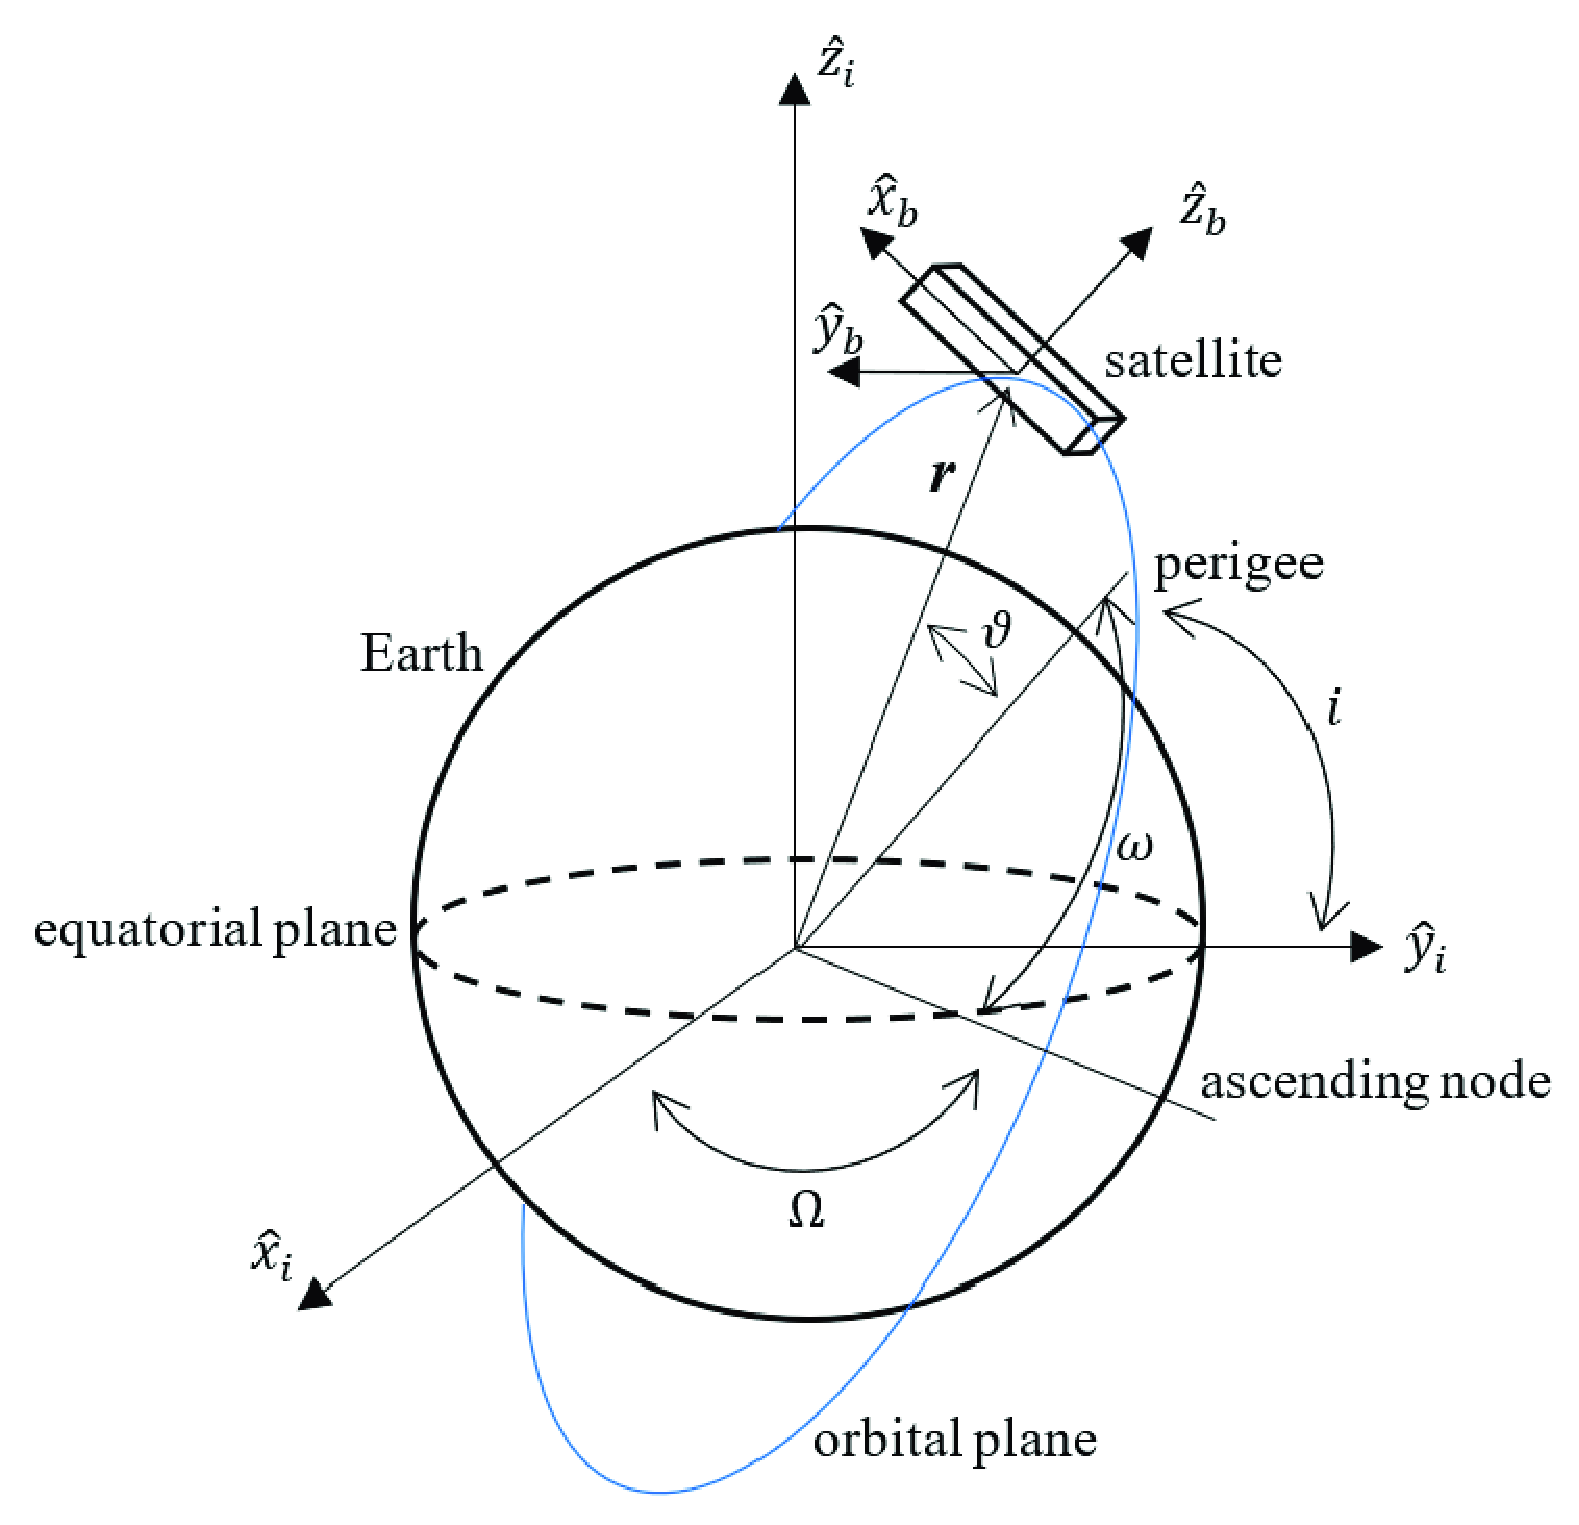
\includegraphics[width=0.85\textwidth]{gfx/gci.eps}
  \caption{\acrfull{gci} frame}
  \label{fig:raytracing}
\end{figure}

The chaser and target body-fixed frames have their origins at the \acrshort{cg} of both, respectively, and their axes are considered to be aligned with their respective principal axes. The origin of the camera frame instead coincides with the center of perspective projection. The target model frame is fixed with respect to the body frame and often coincides with it. For what concerns this work, for the sake of simplicity and without loss of generality, we will consider the camera frame to be coincident with the chaser body-fixed frame, and the target model frame to be coincident with the target body-fixed frame. 

\section{Image generation}
The use of artificial images gives a complete control over the scene. For the purpose of this work, a new procedure for the generation of realistic images, representative of a data-set taken by a monocular navigation camera during a close-proximity approach to target \acrshort{sc} has been developed.
Using the illustrated procedure, the user is able to create synthetic images of a target \acrshort{sc} given it's \acrshort{stl} model, by fine tuning all the properties of the materials composing the target \acrshort{sc}.
Since there could be also cases in which the Earth can be behind the target \acrshort{sc}, the developed tool is also able to simulate Earth's presence at any given location. The tool is also able to the simulate the the atmosphere of the Earth and the cloud layer \cite{jacopo}.
The developed tool couples the well known open-source raytracer \acrshort{povray} with MATLAB in order to archive a good degree of realism in the generated images.

\subsection{Ray Tracing}
Ray tracing is a rendering technique used for generating artificial images which relies on the concept of controlling the path of view lines which starts from the observer camera and ends to generic virtual objects and thus calculating the color intensity of the object.
What is really of crucial importance for our particular use case is that ray tracing is capable of re-creating some of nature's optical effects through transparent and opaque surfaces as reflection and refraction, scattering, and dispersion phenomena (such as chromatic aberration).
Due to this, ray tracing techniques can generate artificial images with a really high degree of photorealism.
When the ray tracer renders the scene, a ray of light is traced for every pixel of the camera. Typically, each ray must be tested for intersection with some subset of the objects in the scene. Once the ray has intercepted an object, the ray tracing algorithm will estimate the amount and the type of incoming light at the point of intersection, examine the material properties and by combining those information will calculate the final color intensity that should be attributed to the pixel.
Several illumination algorithms and reflective or translucent materials may also require more rays to be re-cast into the scene in order to do the necessary computations.
At first glance may seem cumbersome to start the ray from the observer towards the object rather than casting rays to the camera (as is in reality). However, doing so speeds up a lot the computation time, as most of the light rays present in a scene may never reach the eye of the observer, and so, all the time spent for tracing those would be useless.
After either a maximum number of reflections or a ray traveling a certain distance without intersection, the ray ceases to travel and the pixel's value is updated.

\begin{figure}[htbp]
  \centering
  \includegraphics[width=0.85\textwidth]{gfx/scherma-ray-tracing.eps}
  \caption{Raytracing: from the observer to the light source \cite{pictraytracing}}
  \label{fig:raytracing}
\end{figure}

For more information regarding how ray tracing works and ray tracing techniques in general, the interested reader can see \cite{introductionraytracing}.

\subsubsection{Ray tracing with \acrshort{povray}}
\acrshort{povray} is an open-source ray tracing software. It does not offer a GUI for modeling objects, but can be optionally used as Blender rendering engine in order to have a \acrshort{3d} modeling environment to model objects. \acrshort{povray} has also been already used to generate spaceborne imagery. For example, it has been used under the ESA LunarSim study to render images of lunar surfaces. Being an headless executable, \acrshort{povray} can be easily scripted in order to be used in conjunction with other softwares.
\acrshort{povray} gives the programmer several options to customize both the look and feel and the optical properties of the represented objects and the medium that light passes trough. \acrshort{povray} offers the choice to use some predefined geometric shapes, like spheres or cubes; another option instead is to define surfaces of the objects trough meshes. This capability has been used widely by this project to model the spacecraft object.
Any surface can then be characterized by its own optical properties. Every object can have a color specified by an Red Green Blue (RGB) triplet or can be wrapped with a texture.\\
For what concerns light sources, they have no visible shape of their own. They are just points or areas which emit light and can be tuned to accomplish the wanted result. For example we can tune the intensity of the light and the light color by specifying the RGB triplet; any atmospheric effect like opaque gas presence (like smoke or clouds) and its relative optical distortions can be modeled as well.

\subsection{Environment Modeling}
\subsubsection{Earth Modeling}
Earth modeling has been developed in parallel to another thesis \cite{jacopo}.
Here will follow a brief review of how Earth has been modeled taken from \cite{jacopo}.
For modeling the Earth, the \acrshort{povray} \inlinecode{POV}{sphere} object has been used, in conjunction with the \inlinecode{POV}{scale} feature, which allows to make the sphere become an ellipsoid.

\begin{figure}[htbp]
  \centering
  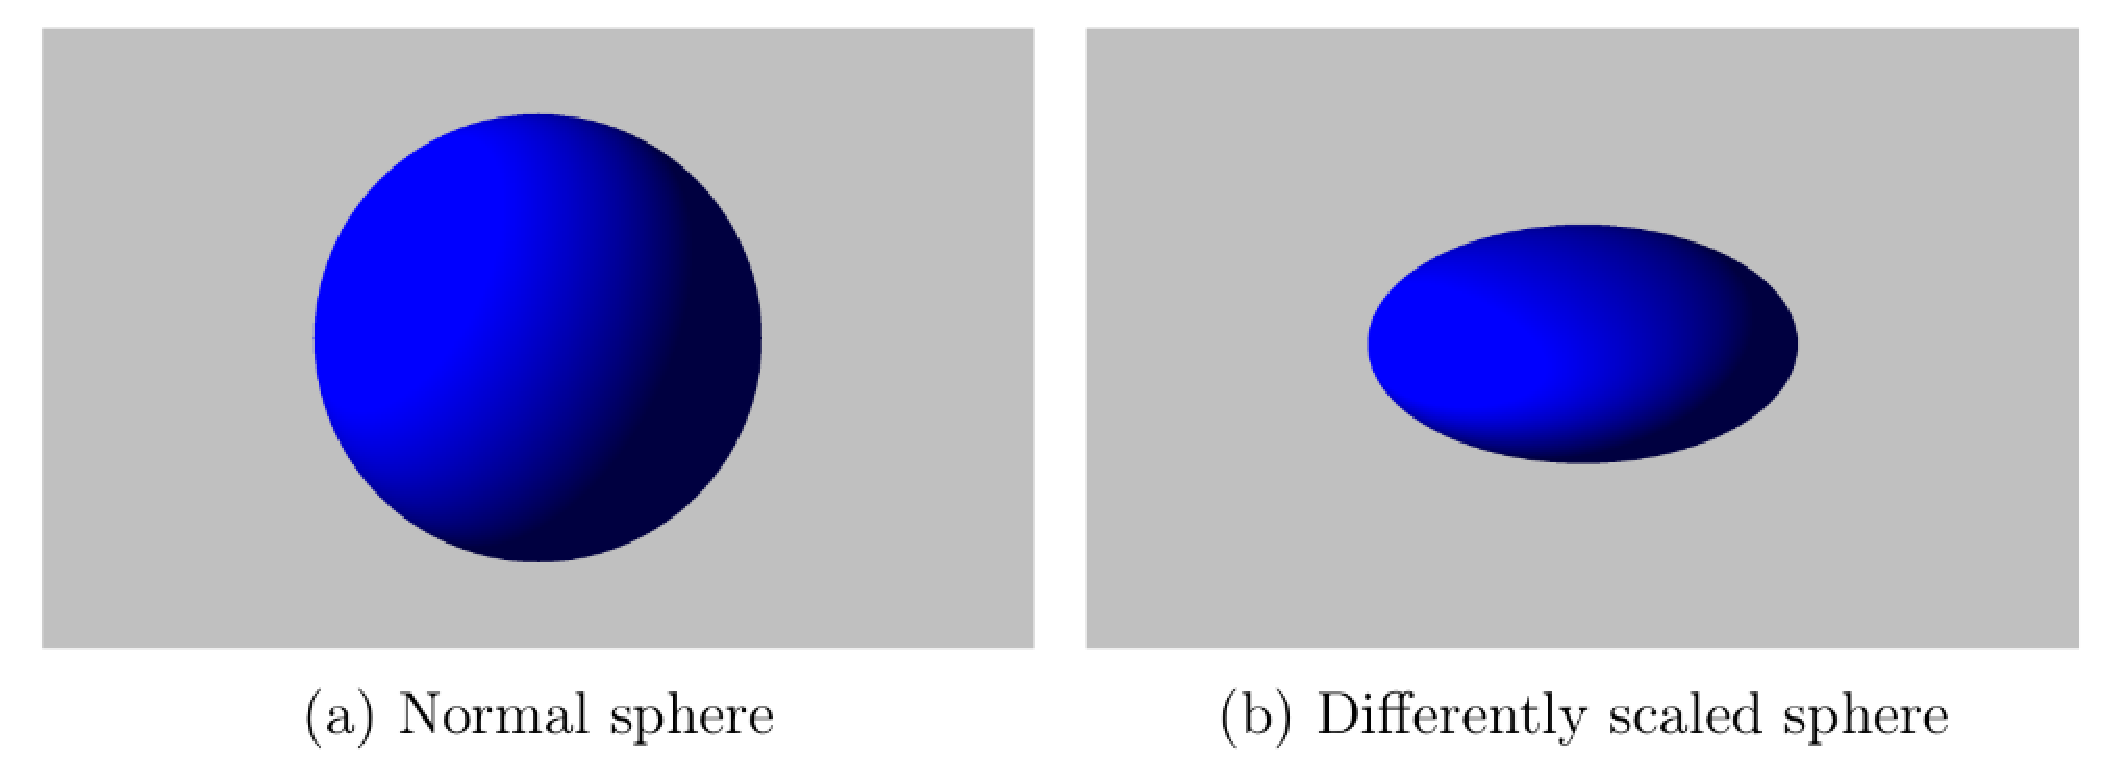
\includegraphics[width=0.85\textwidth]{gfx/sphere_scaling.eps}
  \caption{Sphere manipulation with \acrshort{povray} \cite{jacopo}}
  \label{fig:spherescaling}
\end{figure}

Once the \acrshort{3d} object is created, the most natural choice one can think of is to wrap a \acrshort{2d} texture of the Earth (figure \ref{fig:firstTexture}) on it, and this indeed is what has been done, using an high resolution texture of the Earth.

\begin{figure}[htbp]
  \centering
  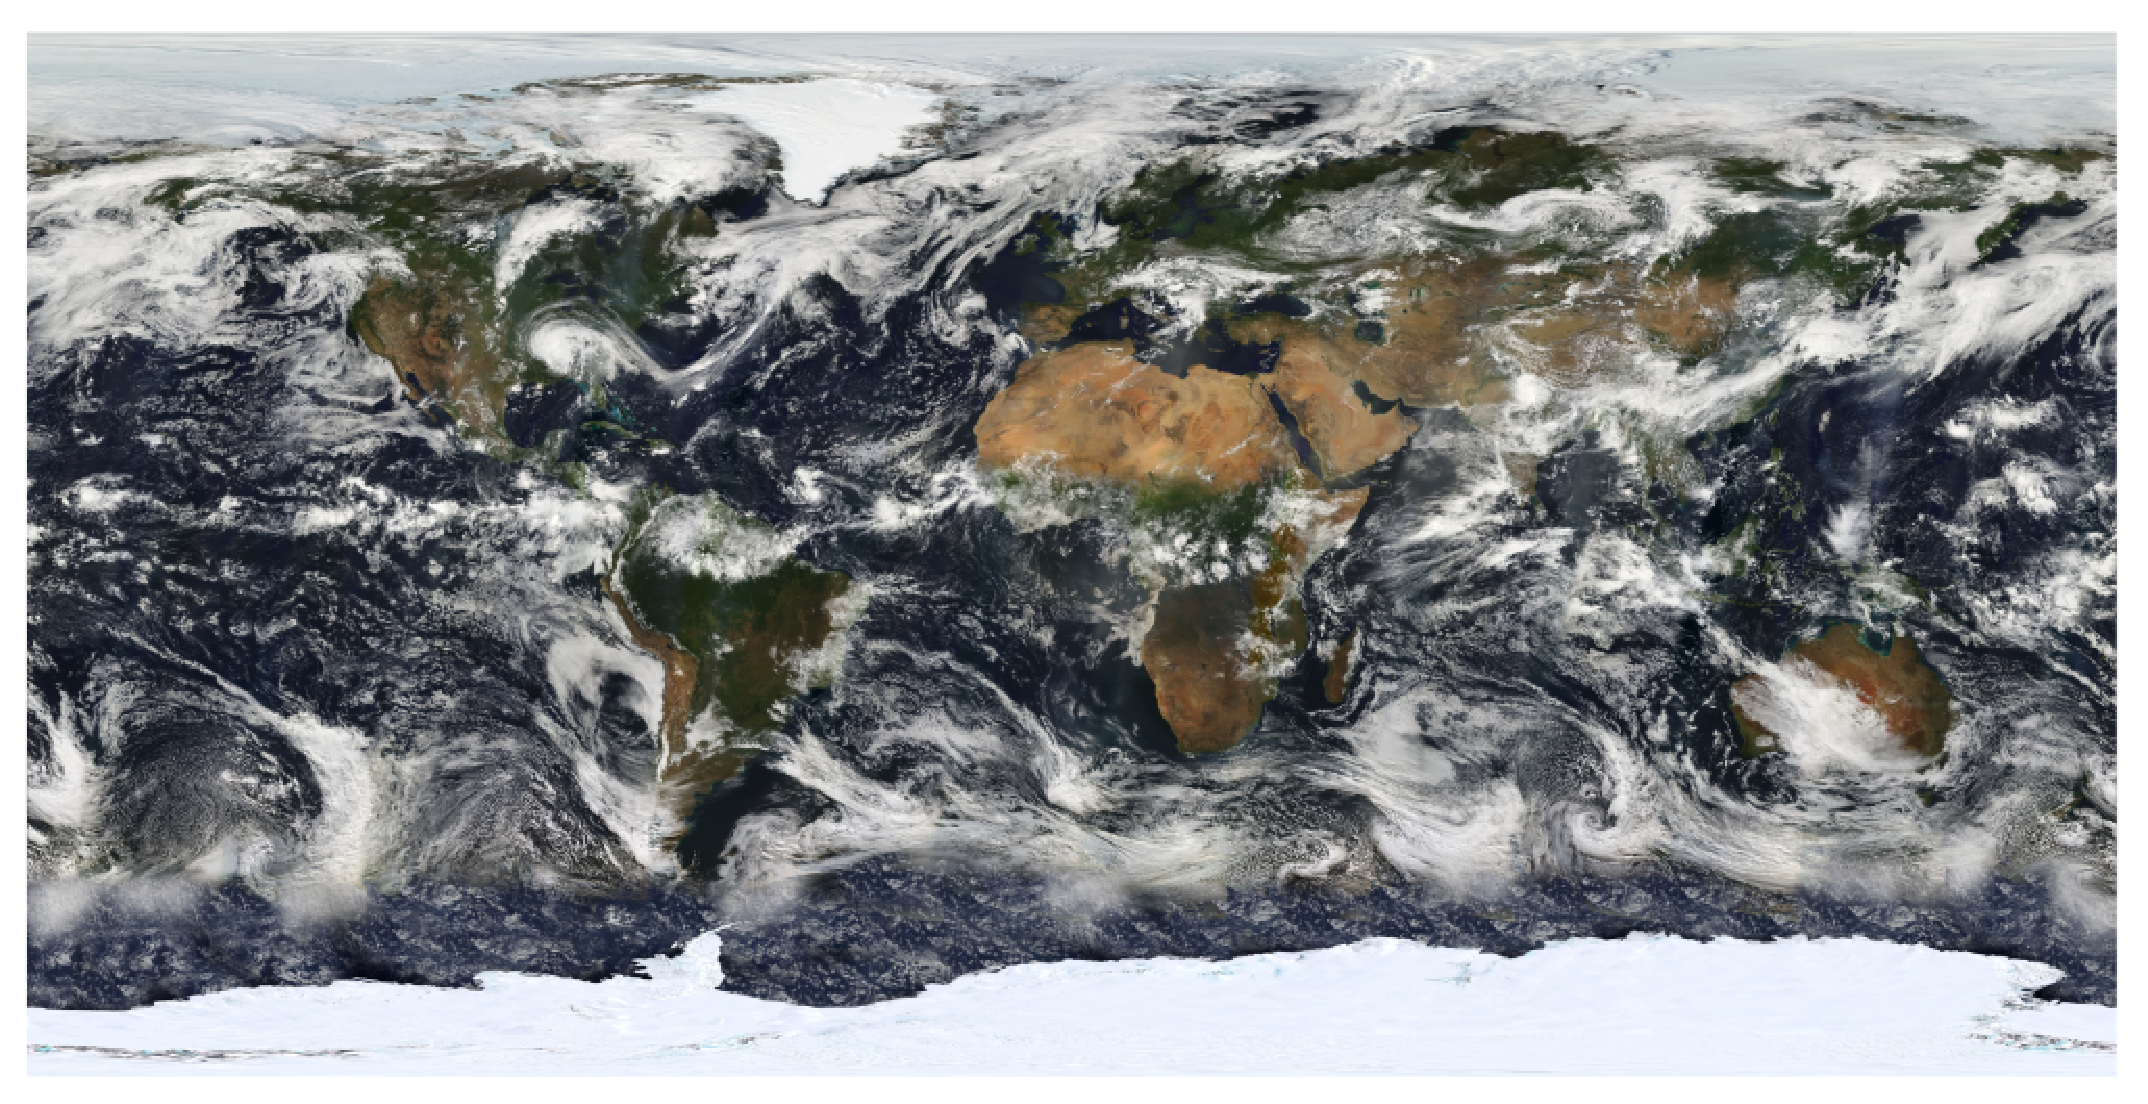
\includegraphics[width=0.85\textwidth]{gfx/first_text.eps}
  \caption{Initially chosen texture of the Earth}
  \label{fig:firstTexture}
\end{figure}

\bigskip

In figure \ref{fig:EarthApollo} we can see a comparison of the synthetically generated image and an actual true image of the Earth as seen from the Apollo 11. From a first glance, used texture gives a good representation of what we should see when we look of a picture of the Earth taken from the space.

\begin{figure}[htbp]
  \centering
  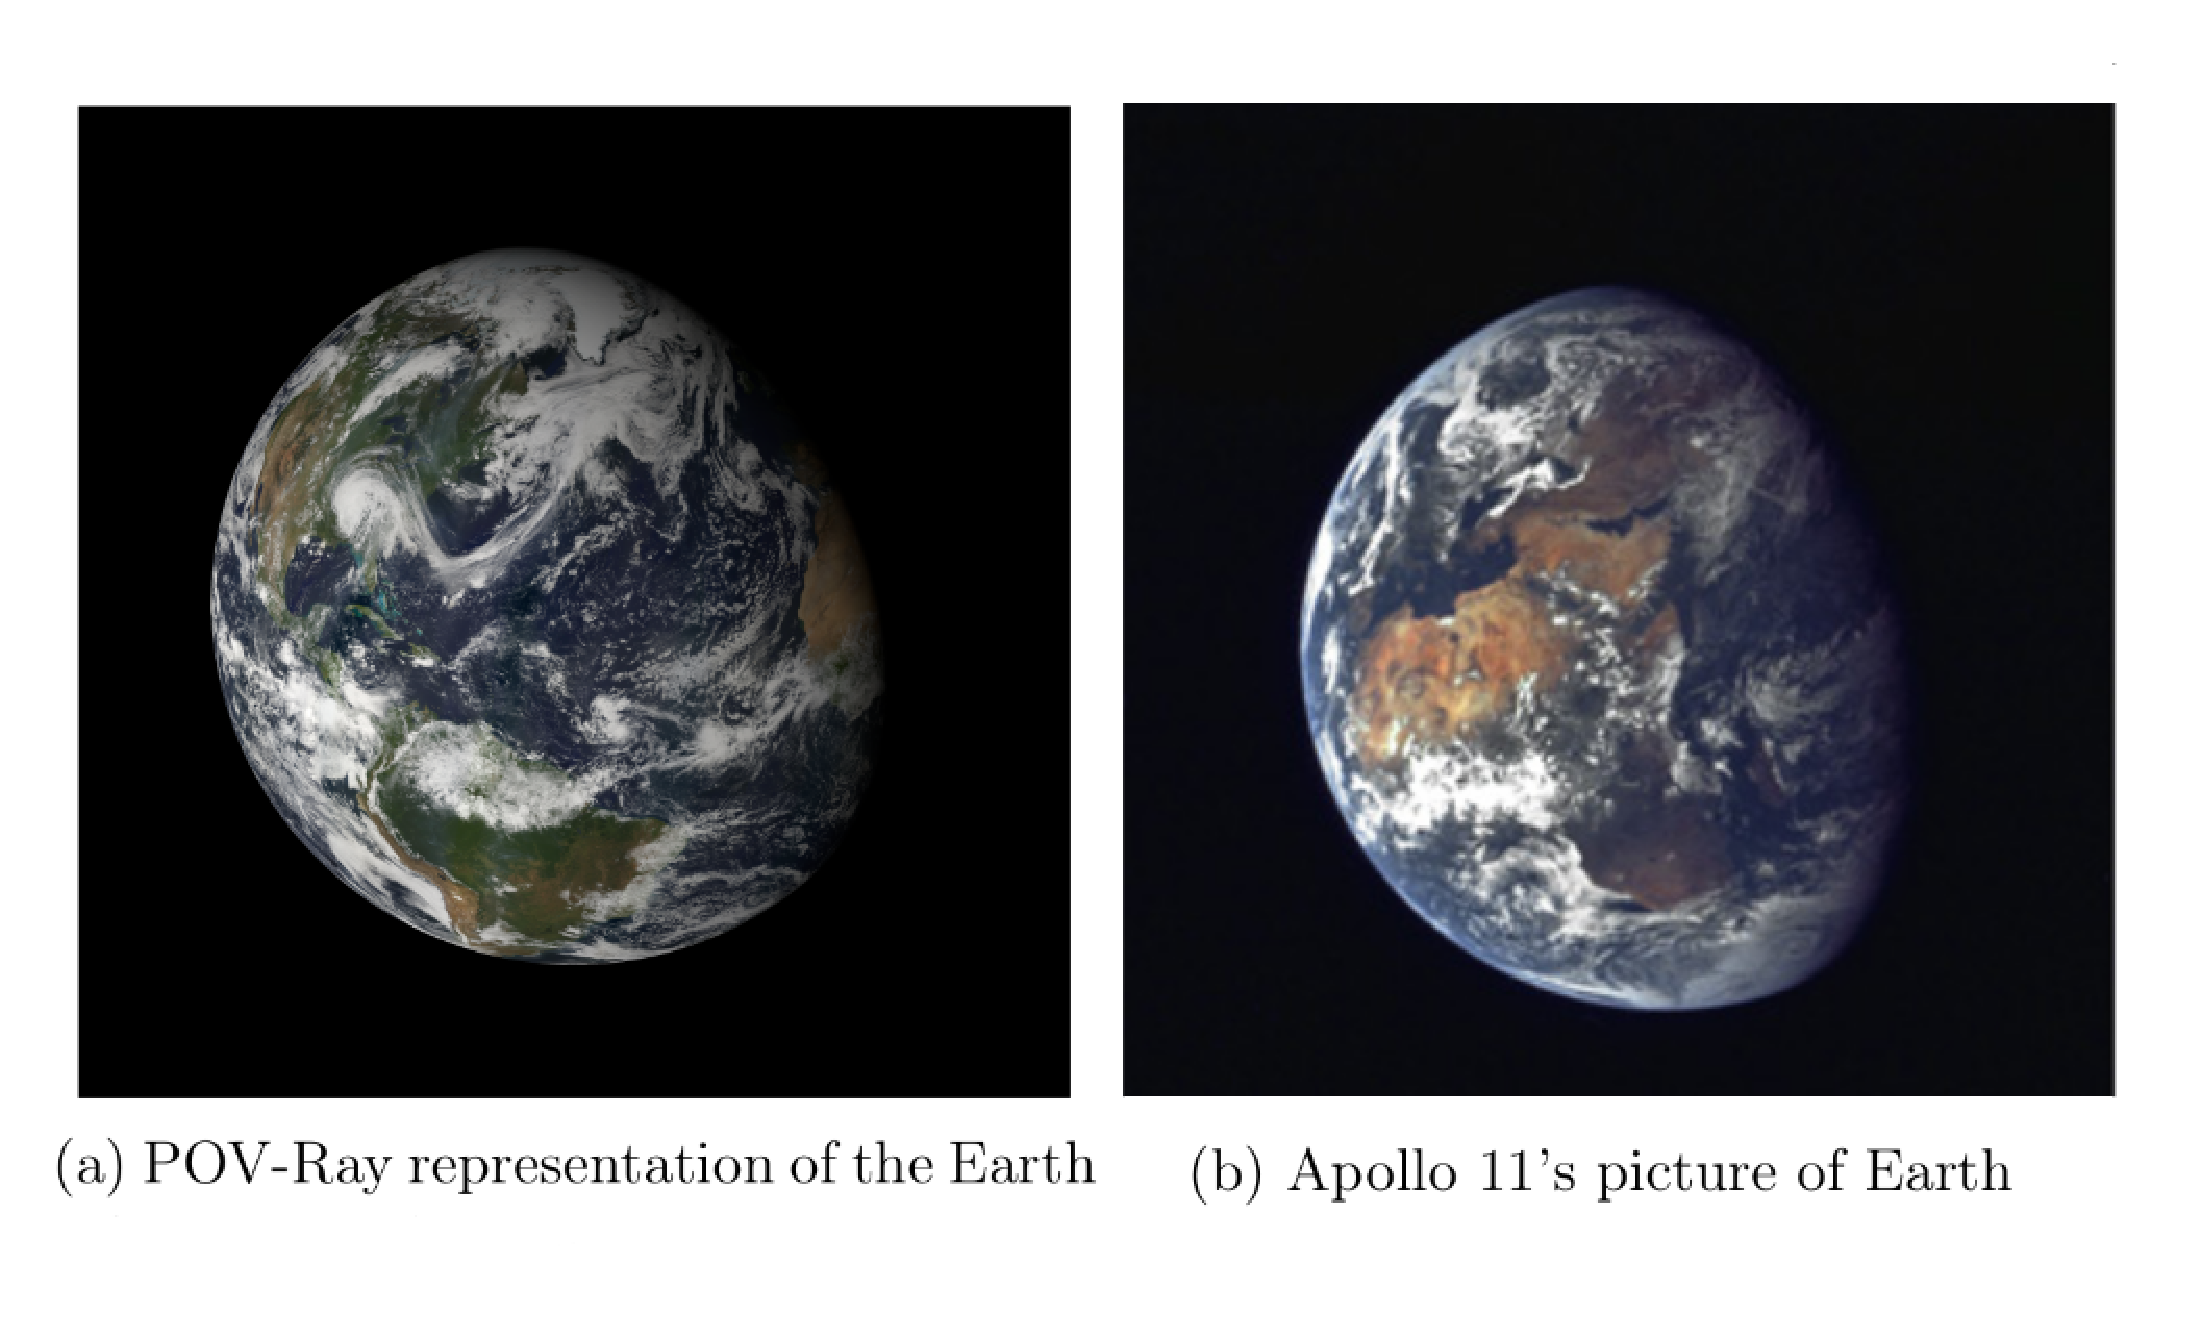
\includegraphics[width=0.85\textwidth]{gfx/earthApolloOurs.eps}
  \caption{Comparison of synthetic Earth image with Apollo 11's picture (the two images have different resolutions)}
  \label{fig:EarthApollo}
\end{figure}

Despite the relatively good result, this way of modeling the Earth still haves some issues :
\begin{itemize}
  \item since for all pictures we use the same texture, the clouds are sticked to their position on top of the surface of the Earth;
  \item terrains and seas are characterized by the same optical properties, while in reality they are not;
  \item diffusion of sunlight in the atmosphere is not simulated;
\end{itemize}
In the following paragraphs, those issues will be addressed.

\paragraph{Cloud Layer}\mbox{}\\
The fixed coupling of Earth surface and clouds is big problem for what concerns CV algorithms development, which should be trained to work in several different conditions, so, having the clouds always on the same region of the Earth despite the orientation is not acceptable.
The solution adopted in both this work and \cite{jacopo} relies on decoupling the Earth terrain layer and the cloud layer, specifying different optical properties for each layer, specify clouds relative rotation with respect to the terrain and coupling back everything together.
Furthermore, oceans have been split too, in order to be able to set different optical properties for the seas.
For the terrain layer, a a true-color mercator image of the Earth has been used as a base, in this way every piece of the surface could possibly be visible in any picture.

\begin{figure}[htbp]
  \centering
  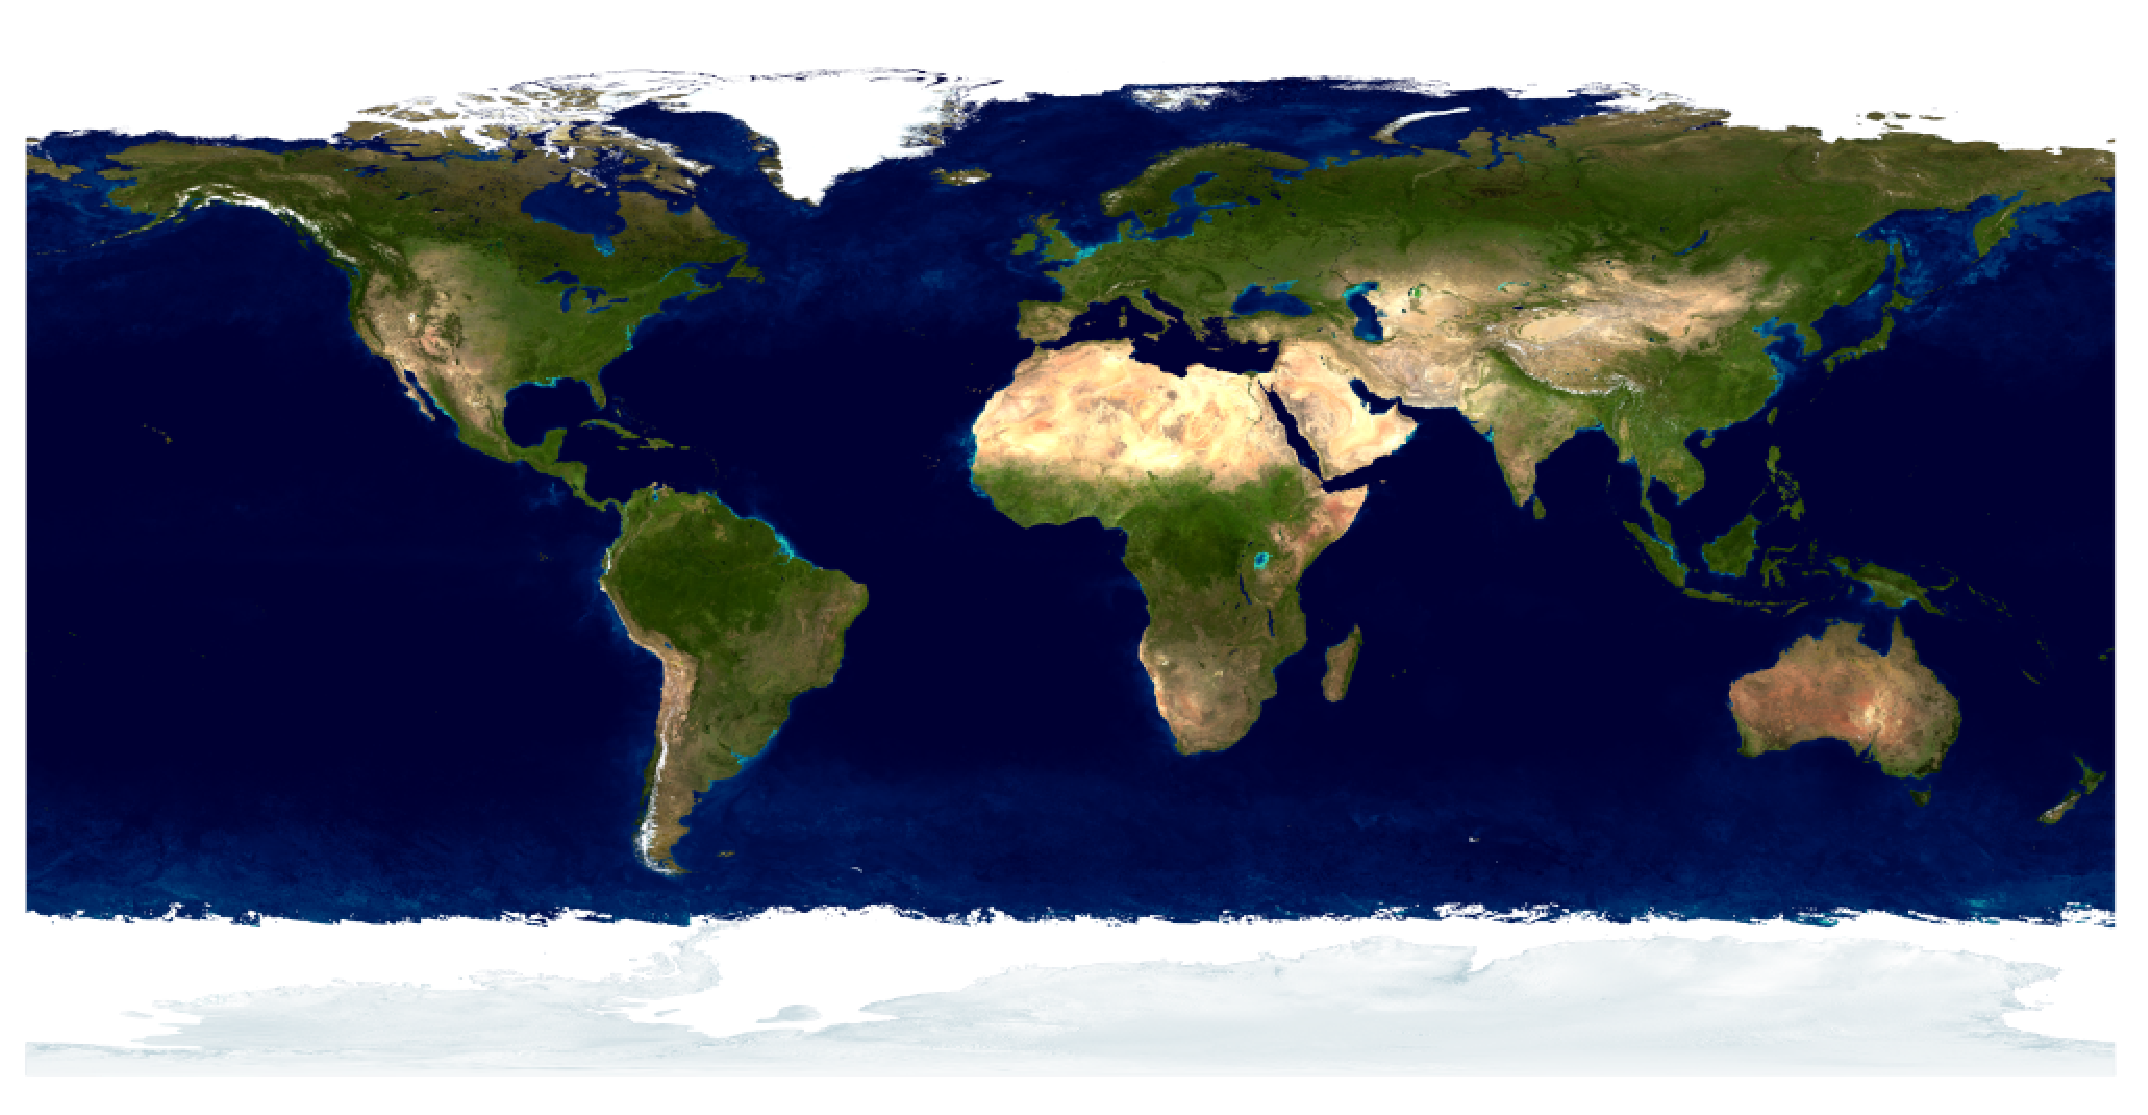
\includegraphics[width=0.85\textwidth]{gfx/earthMercator.eps}
  \caption{True Color Earth Mercator Image \cite{bluemarble}}
  \label{fig:EarthMercator}
\end{figure}

As said before, in order to be able to use different optical properties for water and terrains, a separate two-color mercator-projection image of the Earth where the water is black and the land is white has been used.

\begin{figure}[htbp]
  \centering
  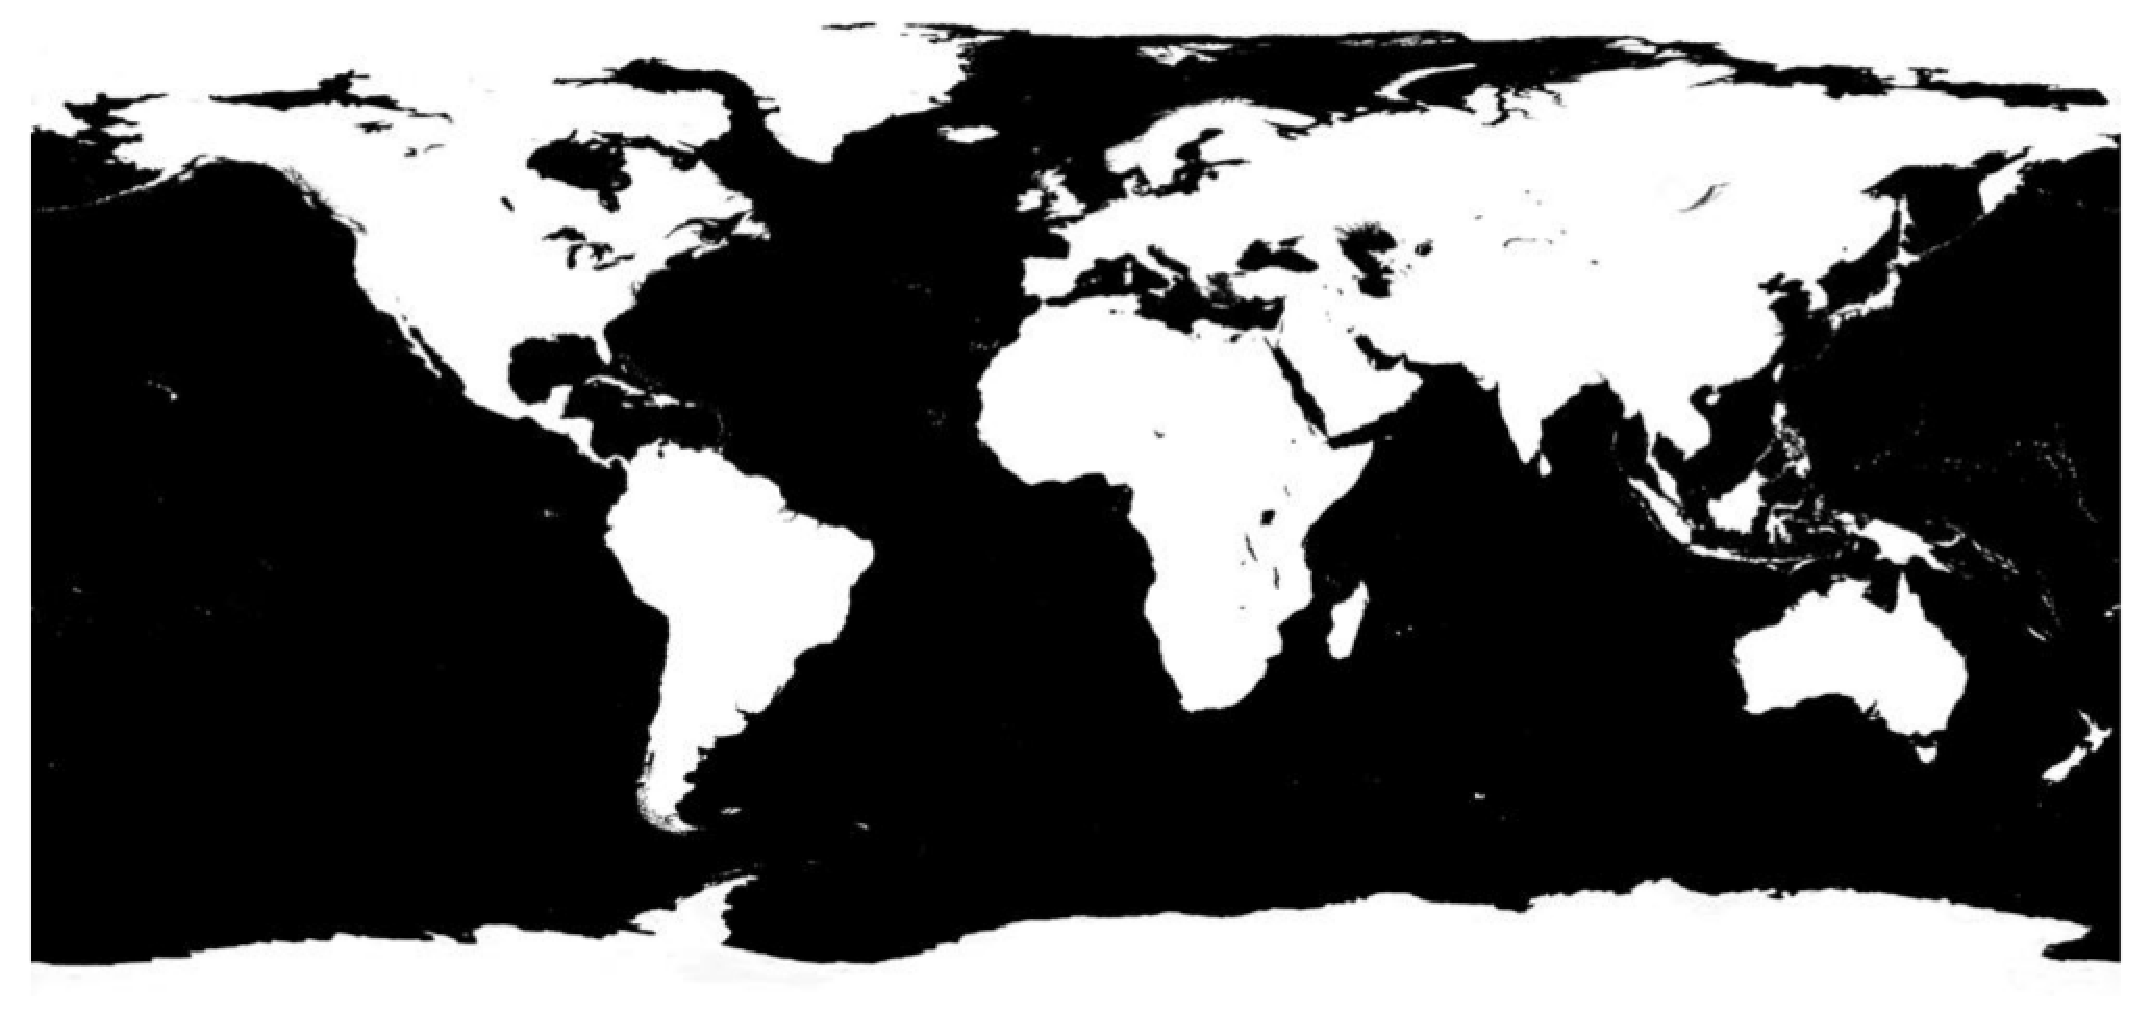
\includegraphics[width=0.85\textwidth]{gfx/landmask_mercator.eps}
  \caption{Landmask Mercator Image}
  \label{fig:LandmaskMercator}
\end{figure}

In figure \ref{fig:comparisonEarths} the result of differentiating the optical properties for terrains and oceans is shown. Despite the fact that it may seems that there is only a small distinction between the two images (in particular, shinier oceans and darker forests), is still enough the make the Earth to seem more photo-realistic, and it leave some space for further tuning.

\begin{figure}[htbp]
  \centering
  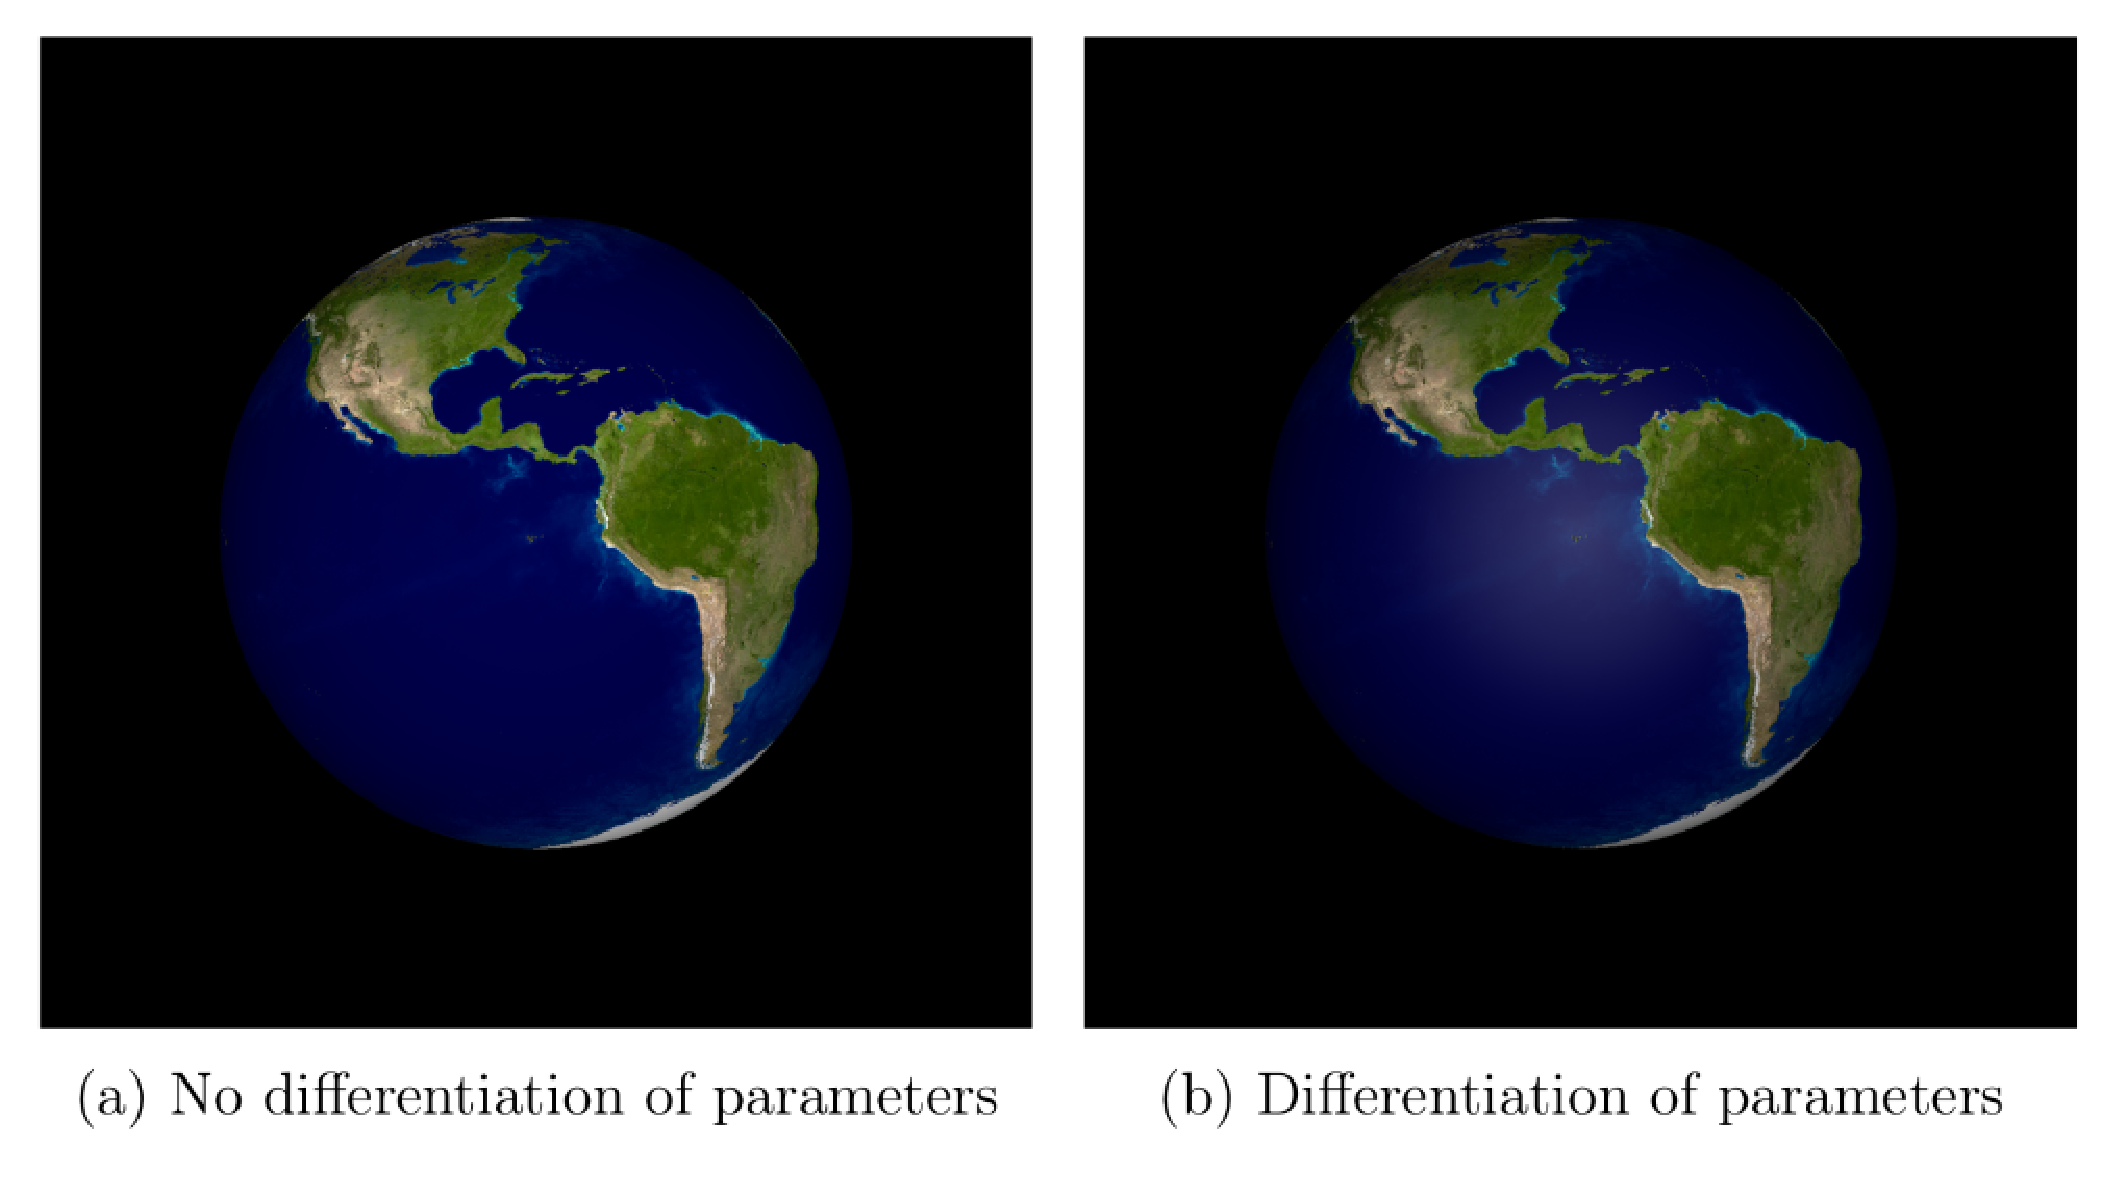
\includegraphics[width=0.82\textwidth]{gfx/comparisonEarths.eps}
  \caption{Comparing images with no differential treatment between land
    and ocean and with differential treatment}
  \label{fig:comparisonEarths}
\end{figure}

The cloud layer is added on top of the cloudless surface and thanks to that, it can rotate with respect to the Earth by a prescribed angle set by the programmer. The cloud layer texture and the shape of the clouds itself always remains the same, but this can be partially mitigated by using different cloud textures.

\begin{figure}[htbp]
  \centering
  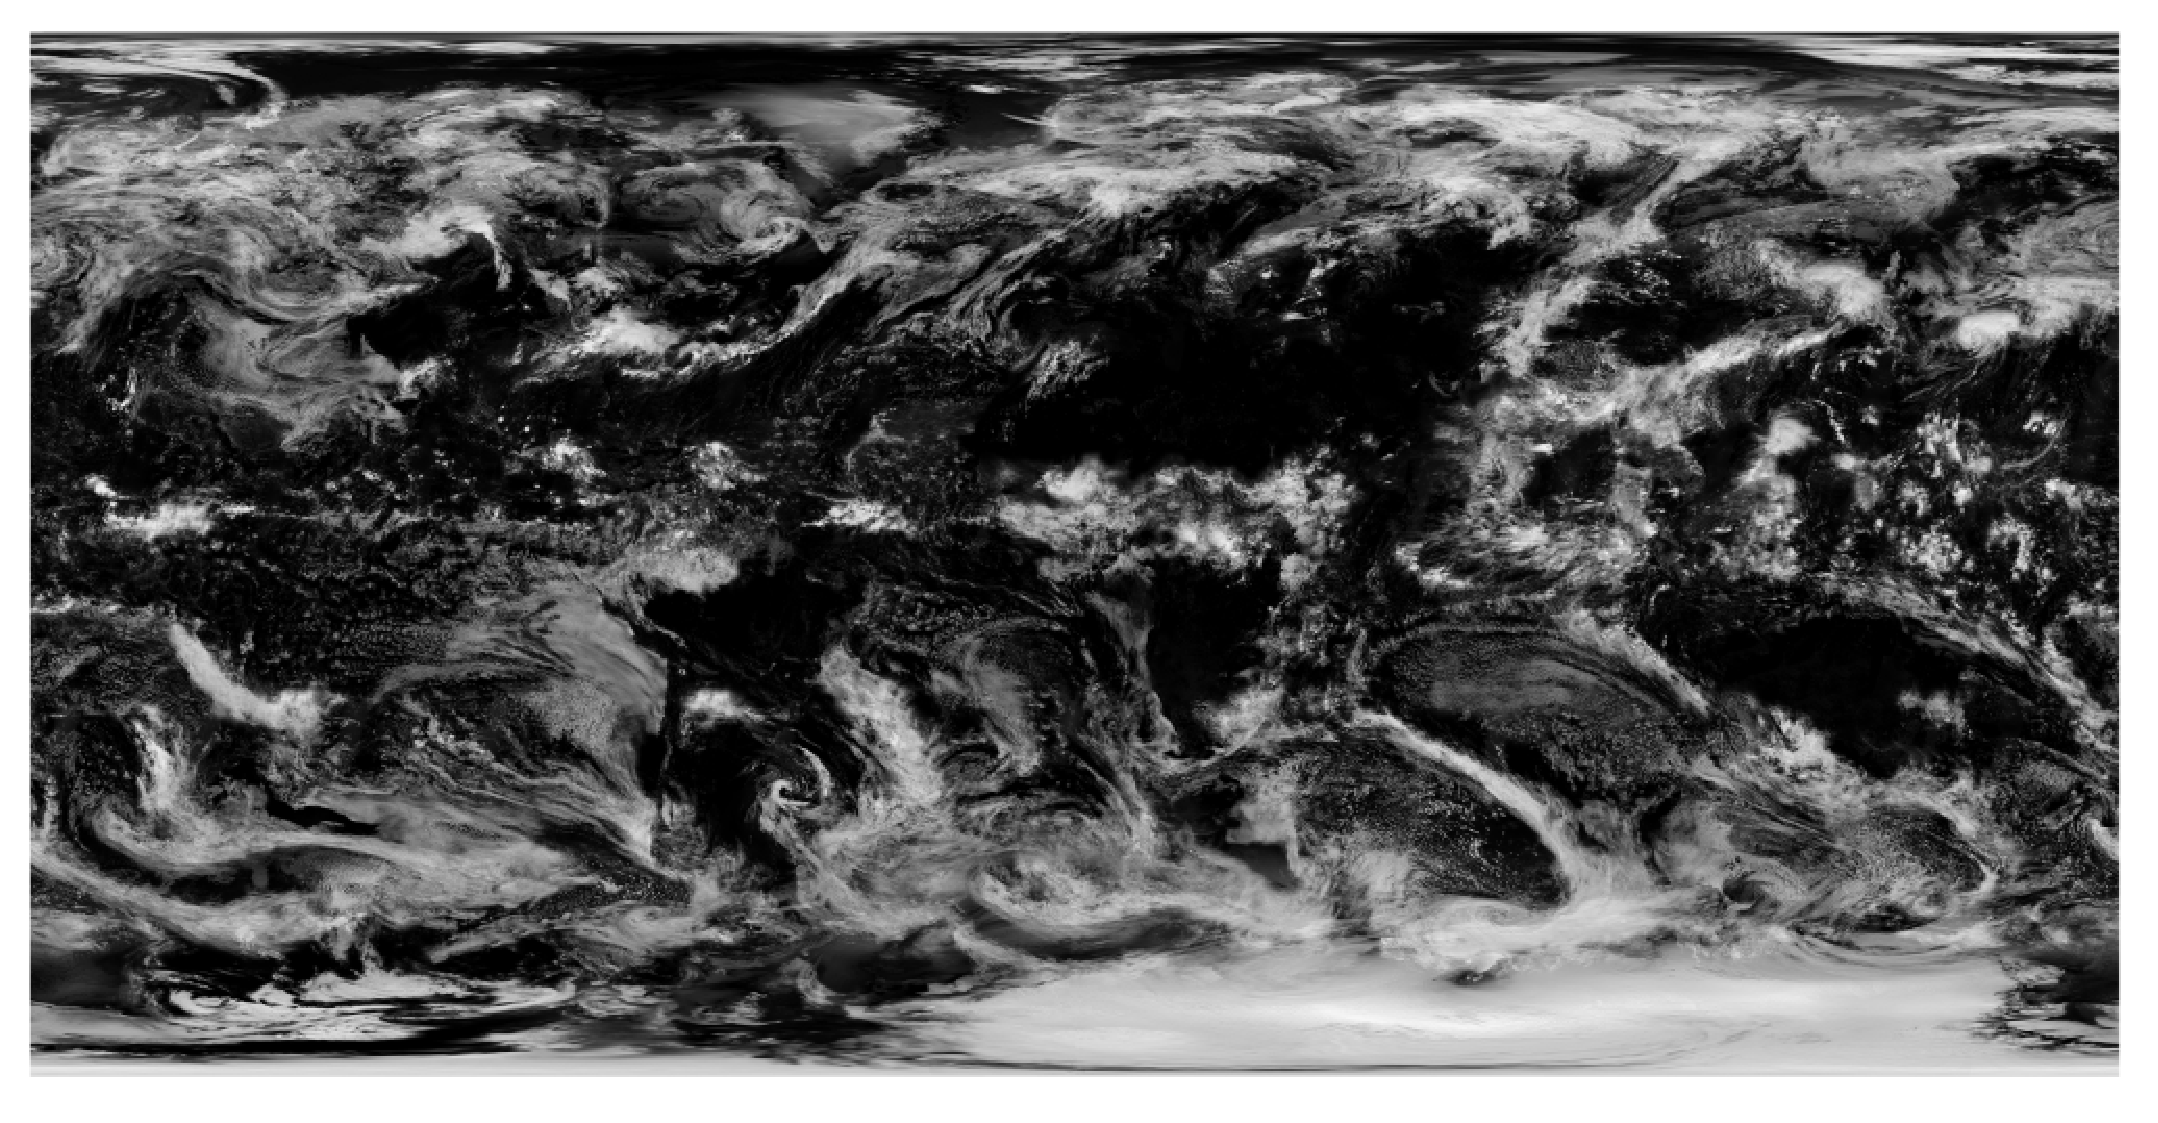
\includegraphics[width=0.85\textwidth]{gfx/clouds.eps}
  \caption{Two-color mercator image of Earth's cloud layer}
  \label{fig:cloudsMercator}
\end{figure}

The cloud texture used for this work (figure \ref{fig:cloudsMercator}) is not actually directly printed on the surface of the earth, but rather is extruded on a shell built around the sphere which defines the Earth, which has an inner radius equal to $R_{in} = 1.001 \cdot R_{Earth}$ and an outer radius equal to $R_{out} = 1.0002 \cdot  R_{Earth}$. Those values have been found by taking as a reference the fact that low Earth clouds ranges from an altitude of \SI{600}{\m} to \SI{15000}{\m} \cite{nimbostratus}. Although higher or thicker clouds can be modeled, this will require longer rendering times. Of course, also for the cloud layer is possible to set custom optical properties, in order to make the clouds partially transparent, so that when there isn't a dense cloud area, the terrain behind is still visible under the white blanket.\\
The result of adding the cloud layer can be seen in figure \ref{fig:cloudShell}

\begin{figure}[htbp]
  \centering
  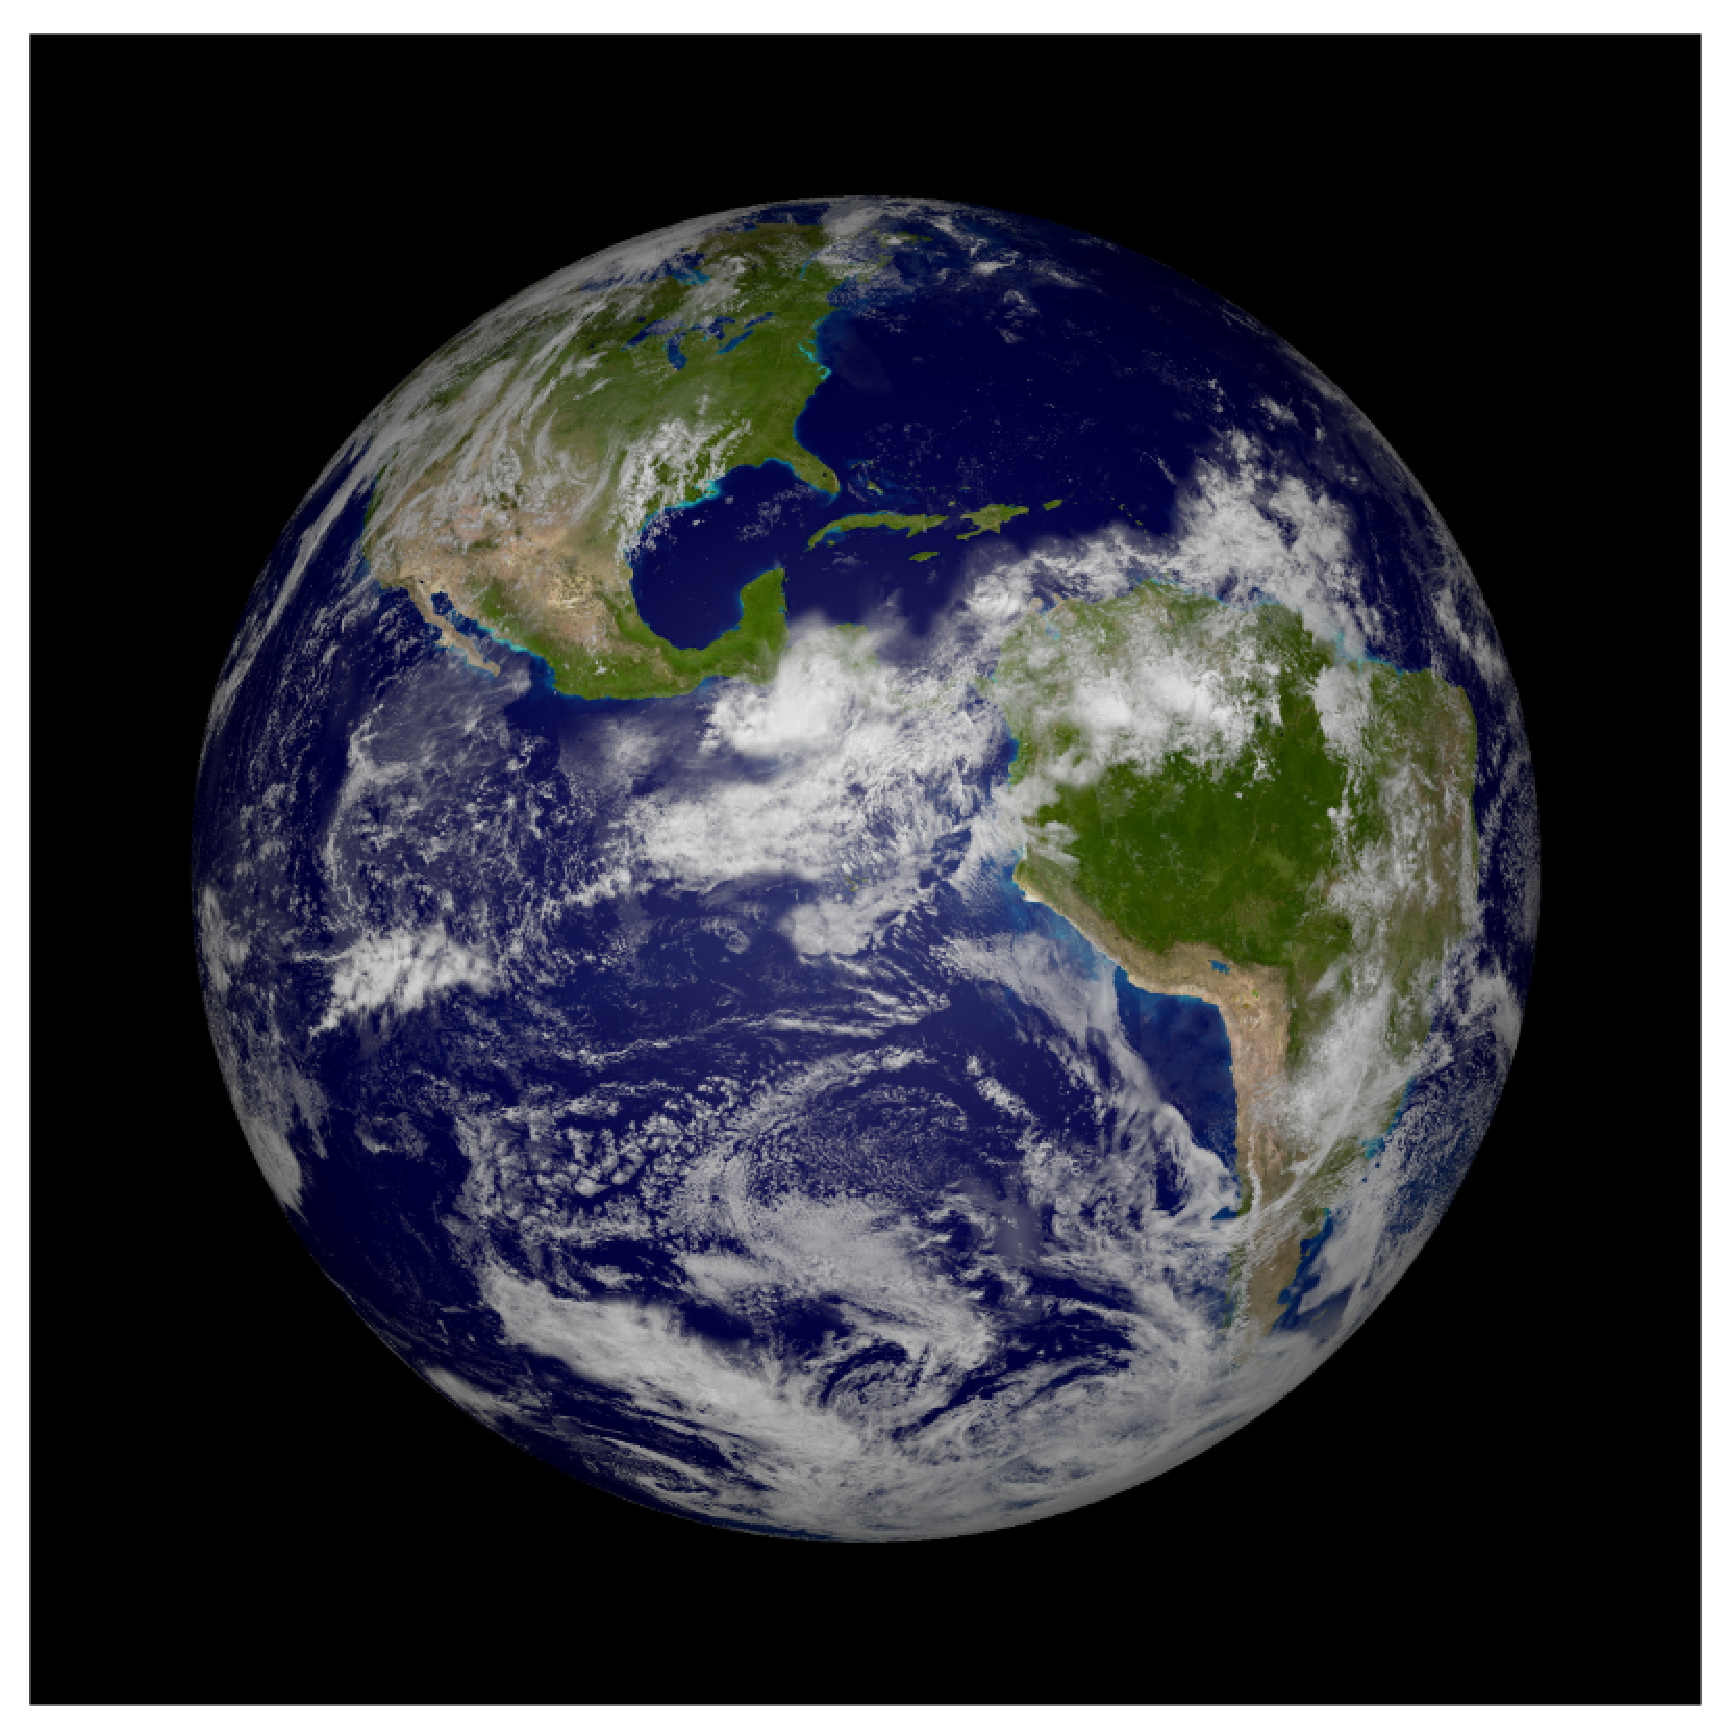
\includegraphics[width=0.72\textwidth]{gfx/cloudShell.eps}
  \caption{Earth's representation using cloud shell}
  \label{fig:cloudShell}
\end{figure}

\paragraph{Cloud Layer}\mbox{}\\
Recreating the characteristic atmosphere presence around the Earth is of crucial importance for developing a CV algorithm for space applications, as it is needed in order to train the algorithm itself to work into a real-case scenario.
The atmosphere's presence in fact would enlarge the aspect of the Earth in the image, and furthermore would stress the edge detection algorithms.
To recreate the atmospheric shine effect, a strategy which is similar to the one adopted to model the cloud layer has been used. In fact, it has been modeled as a shell with a certain thickness of a transparent material with some scattering properties.
For what concerns both this project and what has been done in \cite{jacopo}, the gaseous layer was made only \SI{25}{\km} thick. Despite the fact that the atmosphere should be visible up to many more kilometers, the computational load introduced by rendering a much high atmosphere is not negligible on a standard PC hardware, and so the image generation time would grow up exponentially, making the task of compiling a data-set of thousands of images very time consuming.
In figure \ref{fig:earthAtmo} can be seen the final result of adding the atmospheric model.

\begin{figure}[htbp]
  \centering
  \includegraphics[width=0.72\textwidth]{gfx/earthFinal.eps}
  \caption{Earth with the atmosphere layer}
  \label{fig:earthAtmo}
\end{figure}

In figure \ref{fig:trueVsFake} instead is possible to view the artificially generated next to a real Earth picture taken by NASA's Suomi NPP on January 4, 2012.
It can be seen that, despite the fact that the real image isn't perfectly reproduced (because some other factors should be known in order to be taken into account, such as exposure time), the synthetic image still provide an high degree of similarity with the real one.

\begin{figure}[htbp]
  \centering
  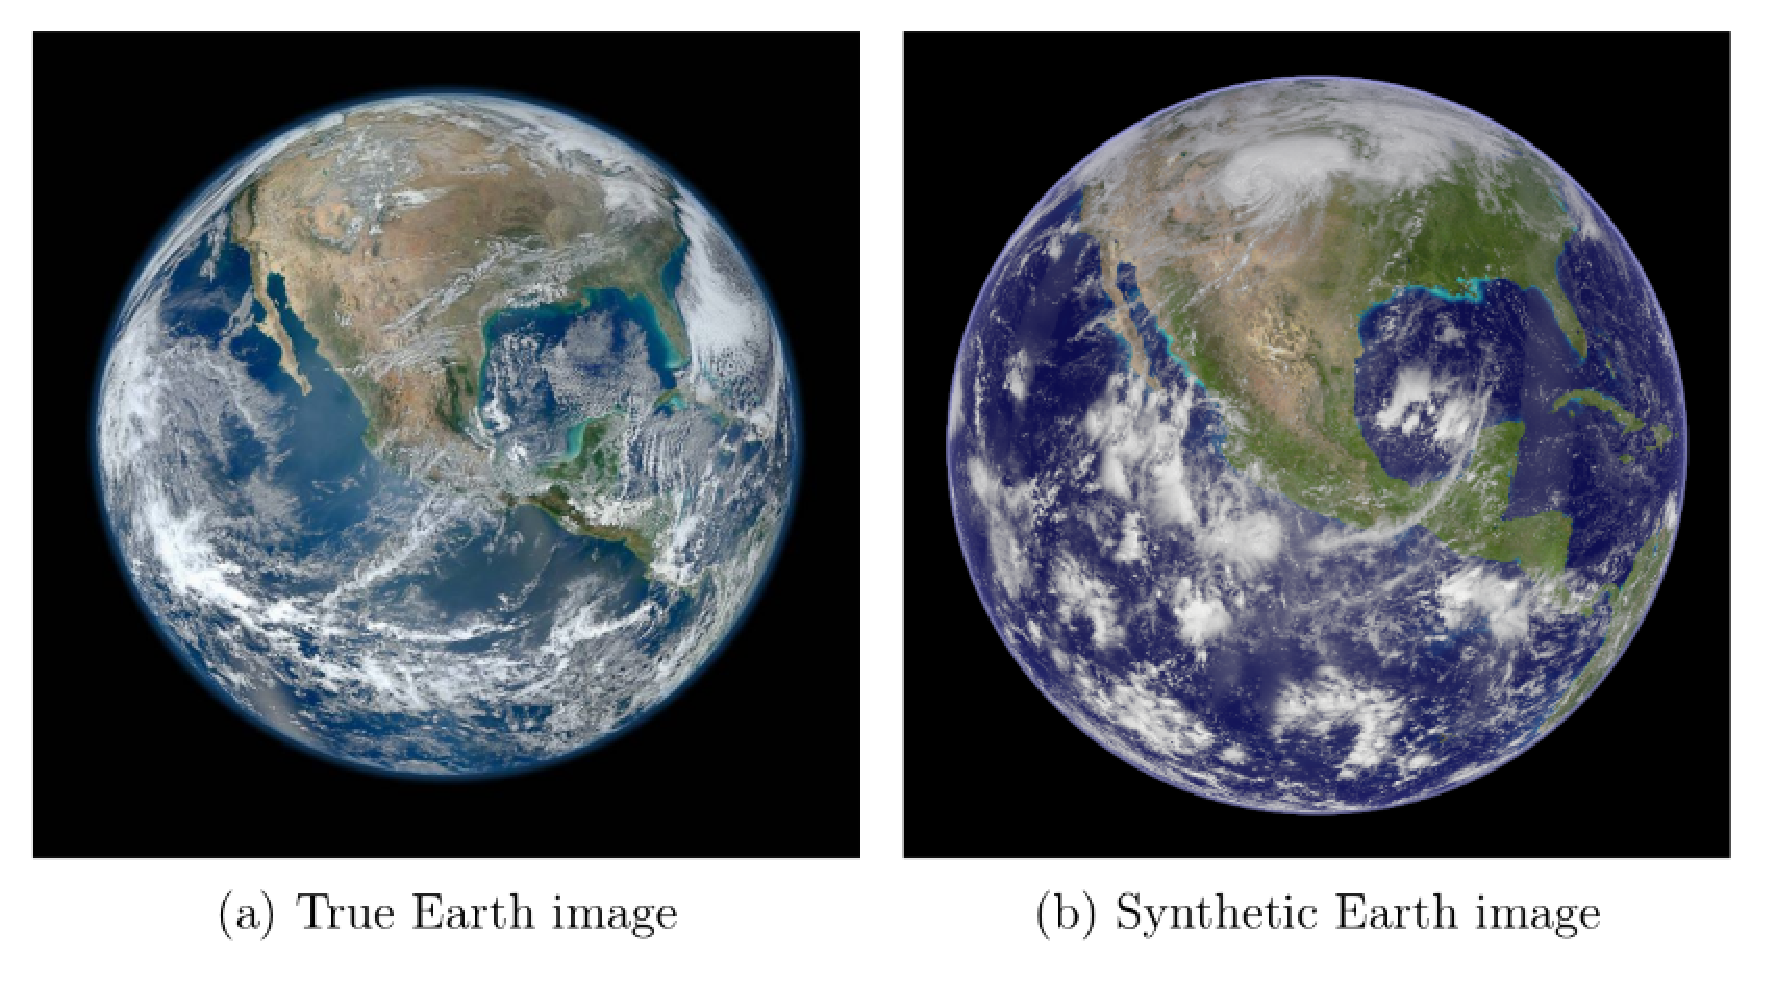
\includegraphics[width=1.0\textwidth]{gfx/trueVsFake.eps}
  \caption{Comparison between true \cite{bluemarble} and final rendered Earth image}
  \label{fig:trueVsFake}
\end{figure}

In table \ref{tab:EarthParameters} are briefly resumed the values used to model the various layer of the Earth.

\begin{table}[htbp]
  \centering
  \begin{tabular}{c cccc}
    \hline
    \hline
               & Terrain & Oceans       & Clouds & Atmosphere \\
    \hline
    Ambient    & 0.001   & 0.001        & 0.001  & 0.0001     \\
    Roughness  & 0.05    & 0.1          & 0.005  & 0.5        \\
    Brillance  & 1       & 1            & 1      & 1          \\
    Diffuse    & 0.85    & 0.85         & 1      & 0.6        \\
    Reflection & 0       & {0.04, 0.25} & 0      & 0          \\
    Specular   & 0       & 0.1          & 0      & 0          \\
    \hline
    \hline
  \end{tabular}
  \caption{Optical parameters of Earth's different layers}
  \label{tab:EarthParameters}
\end{table}

\subsubsection{Light Modeling}
For an object to show up into the scene, it must be illuminated.
There are two ways to illuminate an object with \acrshort{povray}:

\begin{itemize}
  \item use a standard light source
  \item use ambient light
\end{itemize}

The light source is controlled by the keyword \inlinecode{POV}{light_source}, which in turn accepts several modifiers. Light sources in \acrshort{povray}have no visible shape of their own. They are just points or areas which emit light.\\
The ambient light instead is controlled by the keyword \inlinecode{POV}{ambient} added to the \inlinecode{POV}{finish} modifier of an object, and it is used to simulate the light inside a shadowed area.
We can think of ambient light like a kind of light that is scattered everywhere in the room. It bounces all over the place and manages to light objects up a bit even where no light is directly shining.
In our particular case, we can use the \inlinecode{POV}{ambient} option to simulate the illumination of the object due to spurious light sources (such as stars) or reflection from other bodies (like the Moon or other planets).
In order to model the lightning condition of a true solar system, the light source has been modeled to resemble as much as possible the light emitted by the Sun.
The solution adopted in this project and in \cite{jacopo} relies upon modeling the sun as an area light source through the option \inlinecode{POV}{area_light}. This allows to create a cluster of point-like light sources distributed on a disc (simulated by adding the \inlinecode{POV}{circular} option to the area light source) which has radius equal to the radius of the Sun, and placed at the exact distance which the Sun has from the Earth in the \acrshort{gci} frame. In order to cope with the fact that in reality the Sun is equal to a sphere of light and not a disc, the option \inlinecode{POV}{orient} has been used. When using \inlinecode{POV}{orient}, every object in the \acrshort{povray} world would see the Sun's disc as oriented toward it, from any position around it.
Furthermore, the option \inlinecode{POV}{jitter} has been used, which tells the ray-tracer to slightly move the position of each light in the area light to eliminate any shadow banding that may occur.

\subsection{Spacecraft Modeling}

\subsubsection{3D Model of the Spacecraft}\label{sec:3dmodel}
The problem of modeling rather complex shapes with \acrshort{povray}, such as can be a spacecraft, it was one of the most demanding parts of this work, which also required to patch \acrshort{povray} source code, to prevent the ray tracer to forcibly use unnecessary features. Obviously, building the \acrshort{sc} using \acrshort{povray} primitives is a sub-optimal solution, as many different \acrshort{sc} can have different shapes, and modeling them by using simpler shapes each time it is simply not efficient. Furthermore, usually detaled \acrshort{3d} CAD models of \acrshort{sc} are available which can be easily exported into \acrshort{stl} format, so the focus has been putted into trying to understand how to translate those \acrshort{3d} CAD models directly into \acrshort{povray} code.
Several open source and closed source software have been coupled together in order to produce trough \acrshort{povray} a render of a given \acrshort{stl} model.
The procedure will be detailed in the following paragraphs.
The \acrshort{sc} which has been modeled for developing this thesis is heavily inspired by the Tango \acrshort{sc} of the PRISMA mission, by ESA.
The spacecraft has been modeled using the dimensions specified in \cite{Sharma2018}, which will be here reported for ease of reading. The solar panel is represented by a polygon of \SI{570}{\mm} x \SI{759}{\mm}, while the spacecraft body instead is represented by a convex polyhedron of \SI{560}{\mm} x \SI{550}{mm} x \SI{300}{\mm}. The radio frequency antennas length instead is of \SI{204}{\mm}. The origin of the CAD model is located in correspondence of the \acrshort{cg}.\\
Using the aforementioned dimensions, the Tango spacecraft has firstly been reproduced using Autodesk Inventor. The result of the modeling procedure is shown in figure \ref{fig:tango3d}.

\begin{figure}[htbp]
  \centering
  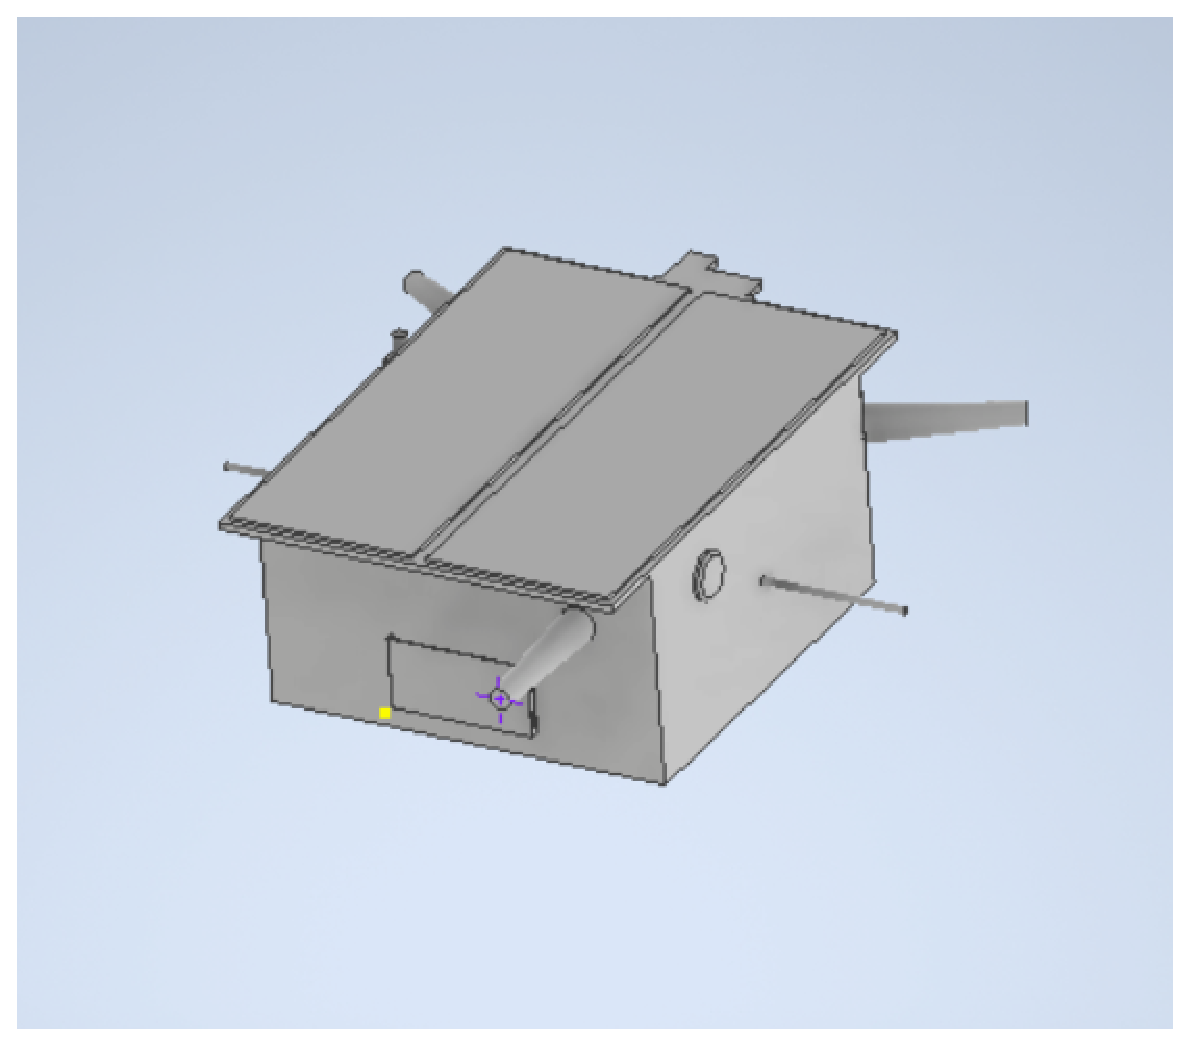
\includegraphics[width=0.62\textwidth]{gfx/tangoScreenshot2.eps}
  \caption{Tango \acrshort{sc} \acrshort{3d} model}
  \label{fig:tango3d}
\end{figure}
The \acrshort{3d} CAD model can now be exported in \acrshort{stl} format to be manipulated through other software.

\subsubsection{Blender}
Once the \acrshort{3d} model of the Tango \acrshort{sc} was available, the most challenging task has been the one of rendering the \acrshort{sc} itself using \acrshort{povray} at attitudes imposed by the user.
The first step for archiving that goal is to import the \acrshort{stl} model of the \acrshort{sc} into Blender. By exploiting the \acrshort{povray} render add-on for Blender, it is possible to render any given \acrshort{stl} file imported file using \acrshort{povray} as rendering engine. The \acrshort{povray} add-on will optionally save the generated SDL code used to render the scene.
The generated code however, will threat the entire \acrshort{3d} model as a whole, generating one giant \acrshort{povray} \inlinecode{POV}{mesh2} object, that is something which cannot be easily managed. Just as an example, would be impossible to assign to the different parts of the \acrshort{sc} different optical parameters or textures.
So, to workaround this limitation, it is a good practice to first split the different surfaces of the \acrshort{3d} model in different different children objects (or children surfaces), and only after render the scene in order to get the POV code. In this way, the \acrshort{povray} render add-on for Blender will generate a \textbf{mesh2} object for each children object created in Blender.
This will enable us to set different material properties for each children surface or to apply different textures to different surfaces.
For the purpose of this work, the original \acrshort{stl} model has been subdivided into thirty children object, each one with its own optical parameters, as can be seen from figure \ref{fig:tangoblender} .

\begin{figure}[htbp]
  \centering
  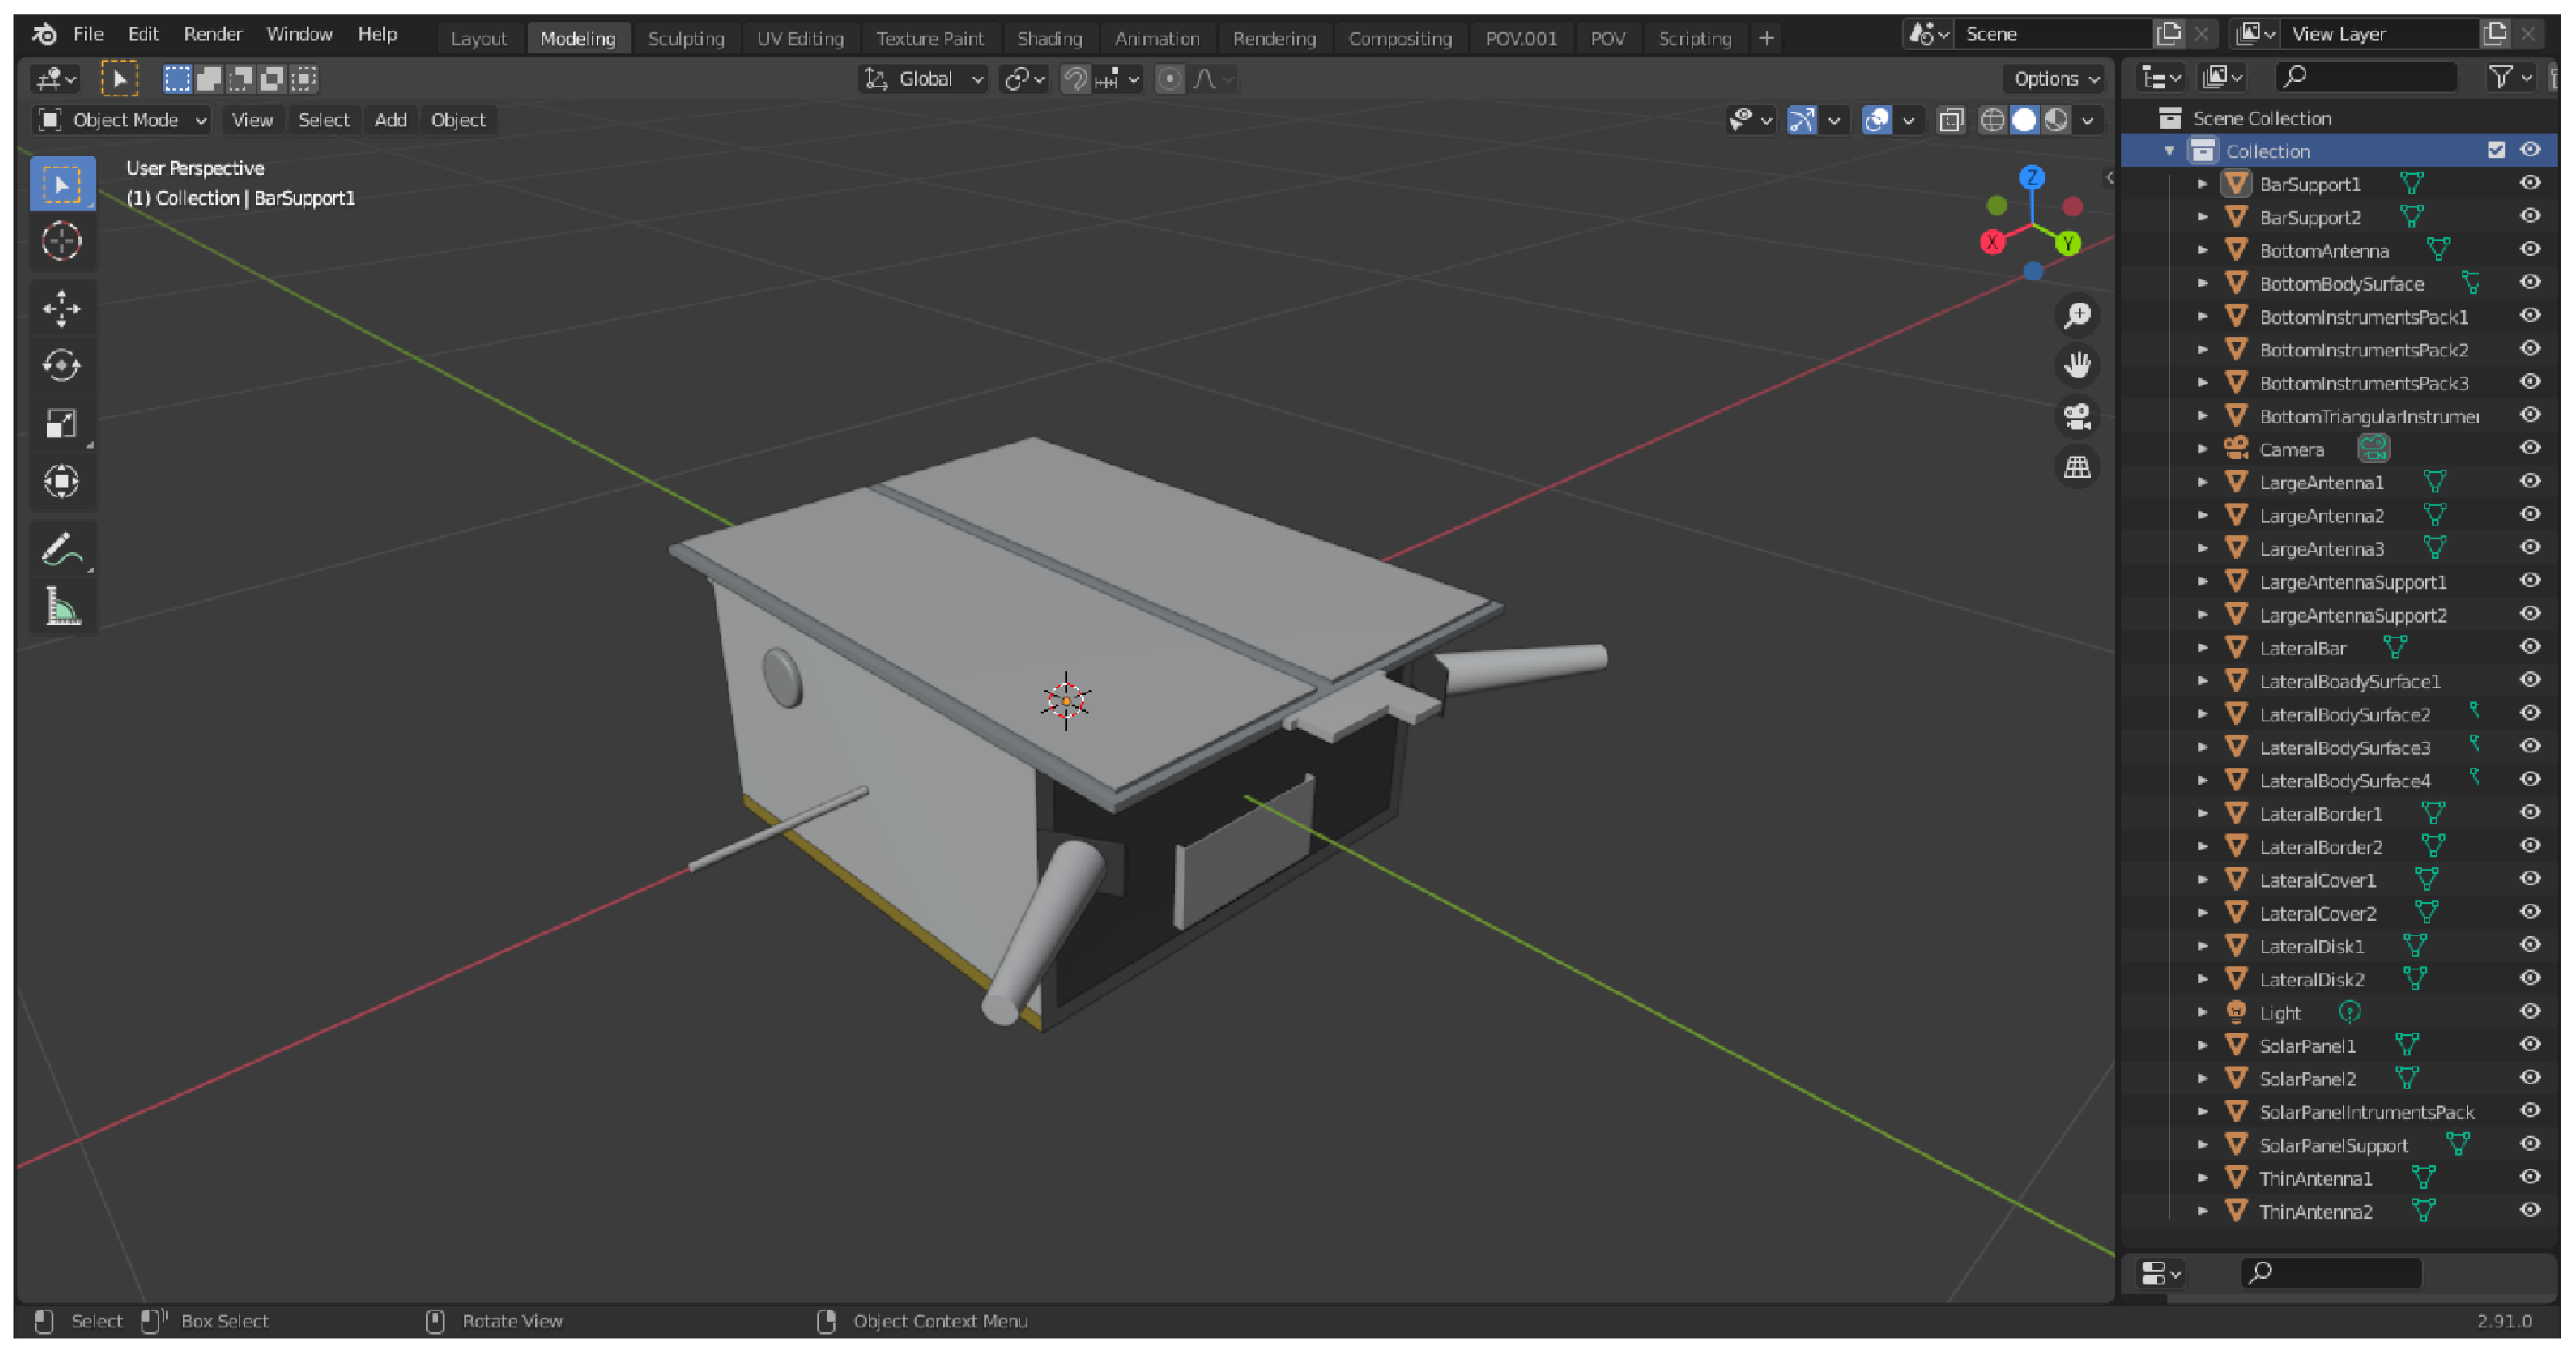
\includegraphics[width=0.82\textwidth]{gfx/tangoBlender.eps}
  \caption{Tango \acrshort{sc} \acrshort{3d} model in Blender}
  \label{fig:tangoblender}
\end{figure}

The Blender \acrshort{povray} add-on also let the user to inject custom POV code (figure \ref{fig:tangoblenderpov}) into the auto-generated one, which can be useful especially for adding textures, for example to the solar panels.

\begin{figure}[htbp]
  \centering
  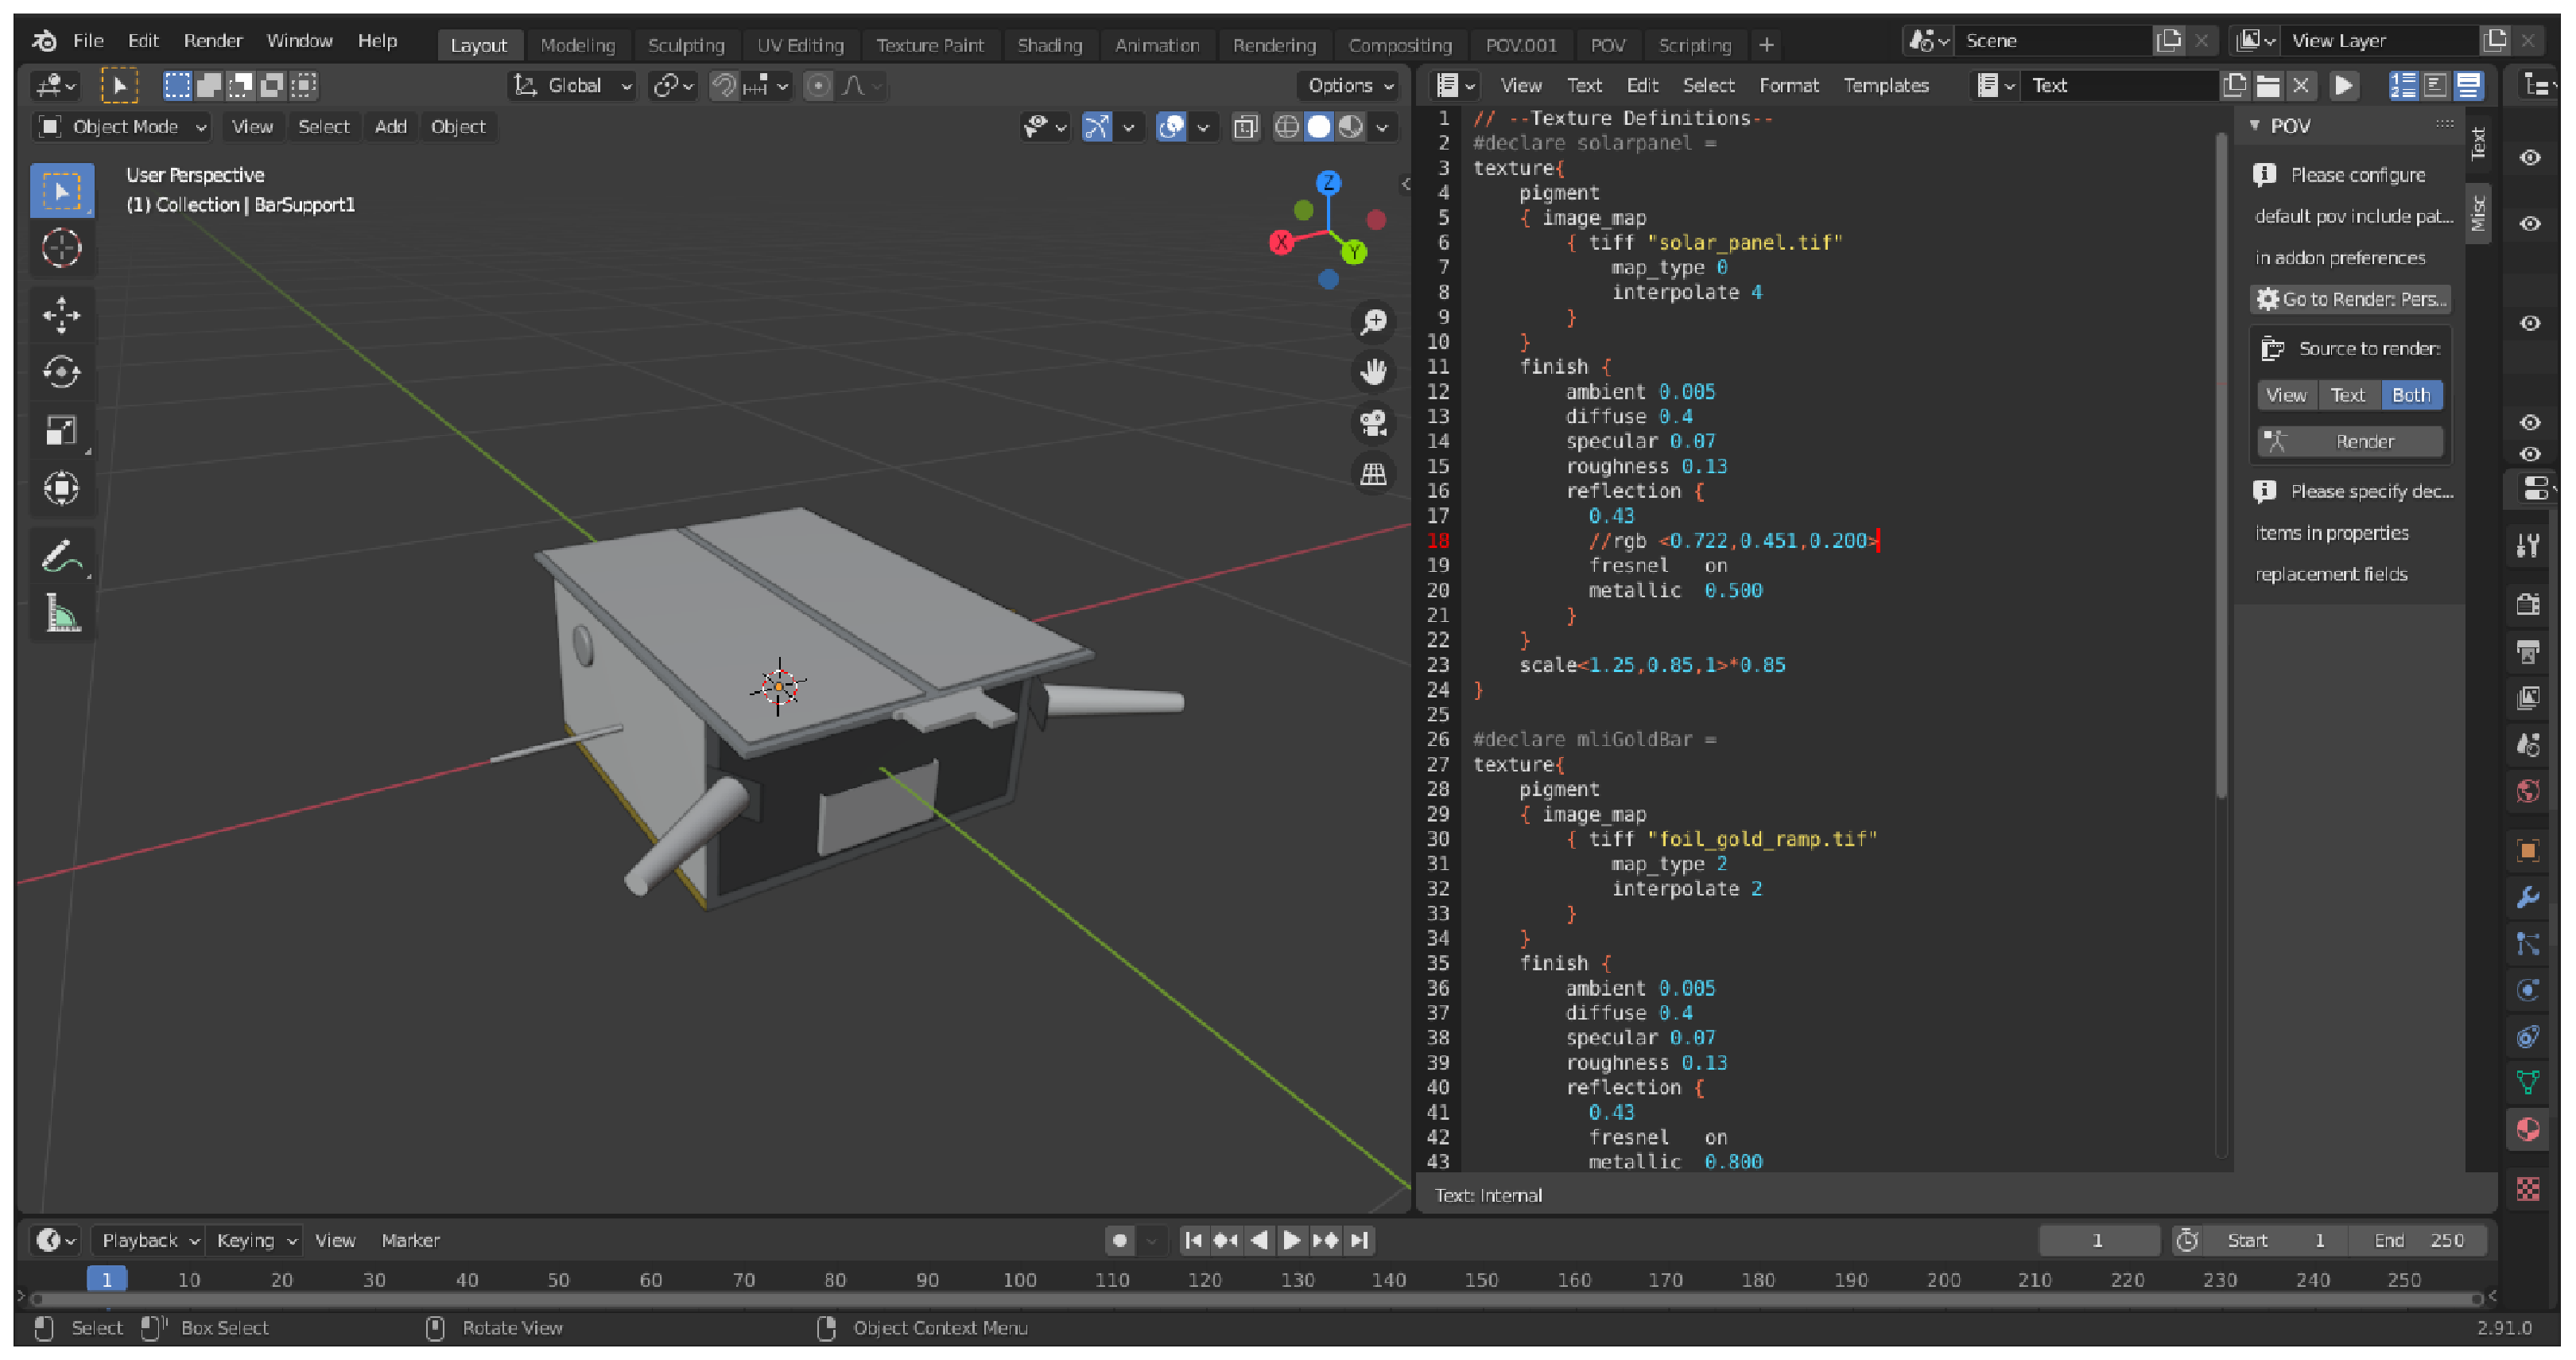
\includegraphics[width=0.82\textwidth]{gfx/tangoBenderPOVCode.eps}
  \caption{Add custom POV code into Blender}
  \label{fig:tangoblenderpov}
\end{figure}

\begin{figure}[htbp]
  \centering
  
\includegraphics[width=0.45\textwidth]{gfx/foil_gold_ramp.eps}
  \caption{Texture used to model MLI}
  \label{fig:mliTexture}
\end{figure}

\begin{figure}[htbp]
  \centering
  \includegraphics[width=0.45\textwidth]{gfx/solar_panel.eps}
  \caption{Texture used to model solar panels}
  \label{fig:solarPanelTexture}
\end{figure}

The end results is showed in figure \ref{fig:tangoblenderfinal}

\begin{figure}[htbp]
  \centering
  \includegraphics[width=0.82\textwidth]{gfx/tangoPolished.eps}
  \caption{Tango \acrshort{sc} rendered using \acrshort{povray} Blender add-on}
  \label{fig:tangoblenderfinal}
\end{figure}

\subsubsection{\acrshort{povray}}
The major issue of the code generated from the  \acrshort{povray} Blender add-on is that is composed of several separated \textbf{mesh2} objects which makes almost impossible to rotate the whole object by imposing a given attitude matrix, since one is supposed to rotate all the \textbf{mesh2} objects by hand.\\
In order to workaround this limitation, from all the \textbf{mesh2} objects which have been generated from \acrshort{povray} Blender add-on are merged into one single \inlinecode{POV}{merge} object.
The \inlinecode{POV}{merge} \acrshort{povray} operation allows to bind two or more shapes into a single entity that can be manipulated as a single object, which is exactly what we want. The new object created by the merge operation can be scaled, translated and rotated as a single shape. The entire merge can share a single texture and optical parameters but each object contained in the union may also have its own texture and optical parameters, which will override any texture statements in the parent object. So, all the \textbf{mesh2} objects which are describing the \acrshort{sc} surfaces are merged into a single big (21K \acrshort{loc}) \textbf{spacecraft} \inlinecode{POV}{merge} object.
To ease the usage of the \inlinecode{POV}{merge} object, a \acrshort{povray} include file it is created, with the sole purpose of containing the \textbf{spacecraft} \inlinecode{POV}{merge} object.
The include file is read in as if it were inserted at that point in the file. Using include is almost the same as cutting and pasting the entire contents of this file into the scene. This allow to define the \textbf{spacecraft} \inlinecode{POV}{merge} once and call it from any other POV file just like any other predefined object is called, and so, it is possible to manipulate its position and orientation in a much more easier way by just using the \inlinecode{POV}{matrix} keyword. The \inlinecode{POV}{matrix} keyword  allows to specify directly the orientation of the \textbf{spacecraft} object, \gls{A_TN}, and its location with respect to \acrshort{povray} "inertial" world.
In table \ref{tab:SCParameters} are briefly resumed the optical parameters used to model the different part of the \acrshort{sc}.

\begin{table}[htbp]
  \centering
  \begin{tabular}{c cccc}
    \hline
    \hline
               & Solar Panels & Antennas  & Main Body \\
    \hline
    Ambient    & 0.0          & 0.25      & 0.25      \\
    Roughness  & 0.13         & 0.0005    & 0.0005    \\
    Brillance  & -            & 3.15      & 3.15      \\
    Diffuse    & 0.3          & 0.95      & 0.99      \\
    Reflection & {0.23, 0.5}  & {0.65, 1} & {0.65, 1} \\
    Specular   & 0.04         & 0.96      & 0.96      \\
    Phong      & -            & 0.43      & 0.43      \\
    Phong Size & -            & 25        & 25        \\
    \hline
    \hline
  \end{tabular}
  \caption{Optical parameters of \acrshort{sc} different parts}
  \label{tab:SCParameters}
\end{table}

\subsection{Camera Modeling}
\acrshort{povray} allows to simulate a perspective pinhole camera (more details about the pinhole camera will be given in section \ref{subsection:pinhole}). In \acrshort{povray}'s camera environment, the programmer can set all relevant camera parameters, which will be then used to simulate the camera trough which the scene will be rendered.
The most meaningful parameters which can be imposed are the location of the camera itself, the direction of the boresight axis (where is the camera looking at), the view angle and the direction of the camera reference frame.\\
The major issue which has been faced when modeling the camera in \acrshort{povray} is the fact that the program defaults to a left handed coordinate system to describe the scene, while all other software (like Autodesk Inventor, Blender) are using a right handed coordinate system.

\begin{figure}[htbp]
  \centering
  \subfloat[\acrshort{povray} axis directions]{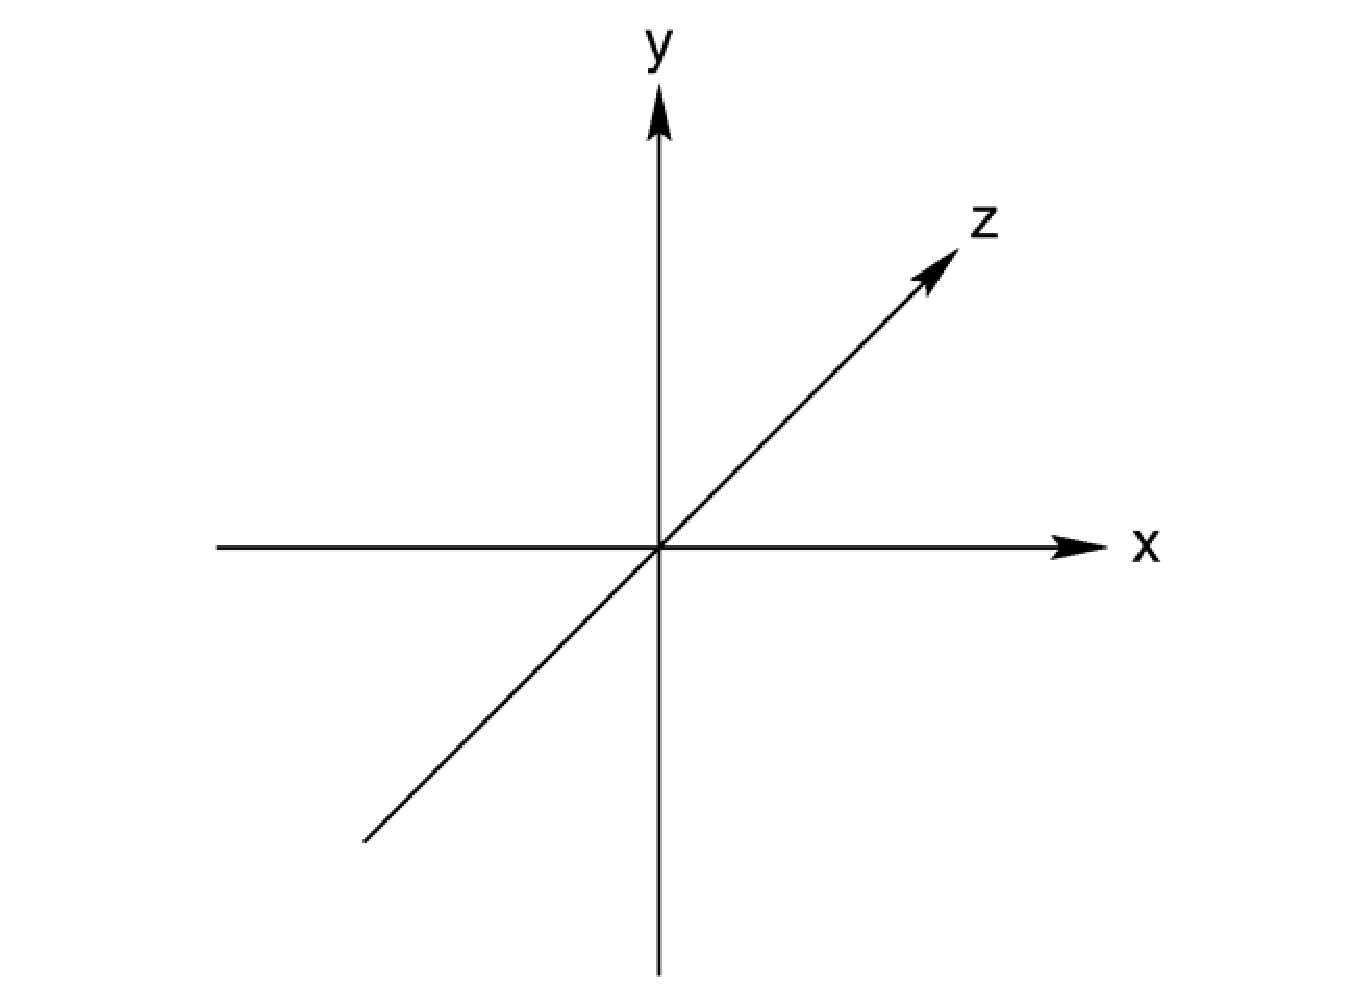
\includegraphics[width=0.4\textwidth]{gfx/povrayTern.eps}}
  \qquad
  \subfloat[Left hand rule]{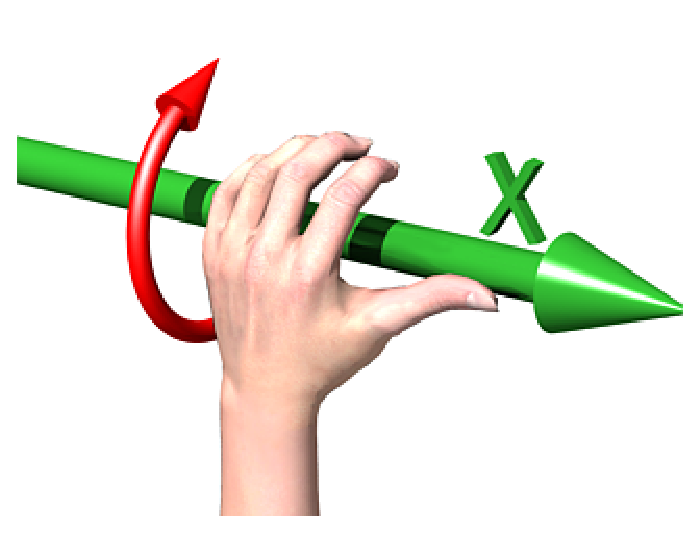
\includegraphics[width=0.4\textwidth]{gfx/povrayHand.eps}}
  \caption{\acrshort{povray} coordinate system}
  \label{fig:povraycoordinatesystem}
\end{figure}

Moreover, the right handed coordinate system is used also to model the orbit that the spacecraft will follow and the spacecraft attitude from Euler equations.
It is possible to trick \acrshort{povray} to behave like it using a right handed coordinate system by acting on the \inlinecode{POV}{right} vector of the camera environment. The camera \inlinecode{POV}{right} vector describes the direction to the right of the camera, so, in practicte, tells \acrshort{povray} where the right side of the screen is. Therefore, the  sign of the x component of the \inlinecode{POV}{right} vector can be used to determine the handedness of the coordinate system in use.

\begin{figure}[htbp]
  \centering
  \subfloat[Left Handed Coordinate System]{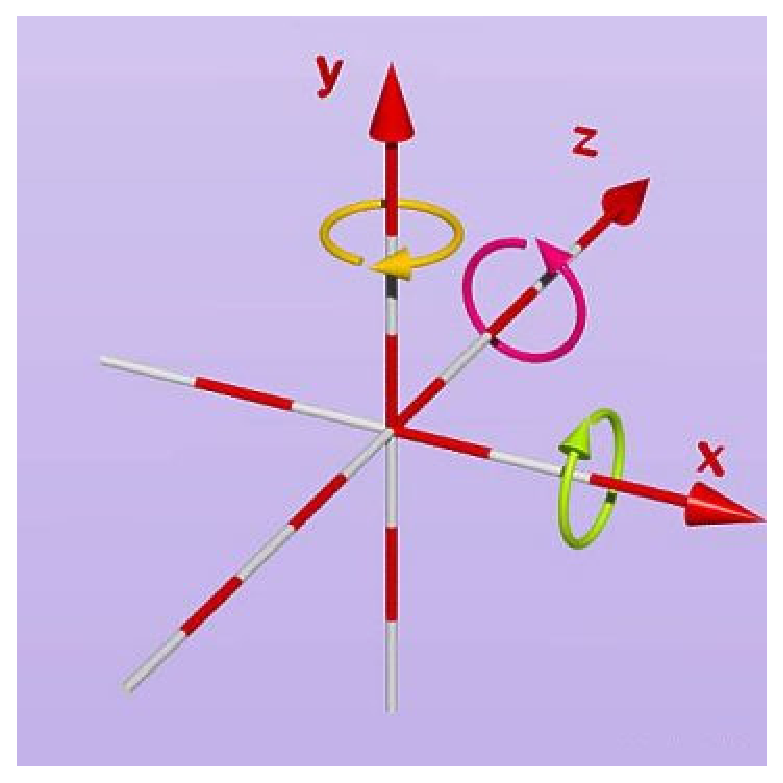
\includegraphics[width=0.4\textwidth]{gfx/axesLeft.eps}}
  \qquad
  \subfloat[Right Handed Coordinate System]{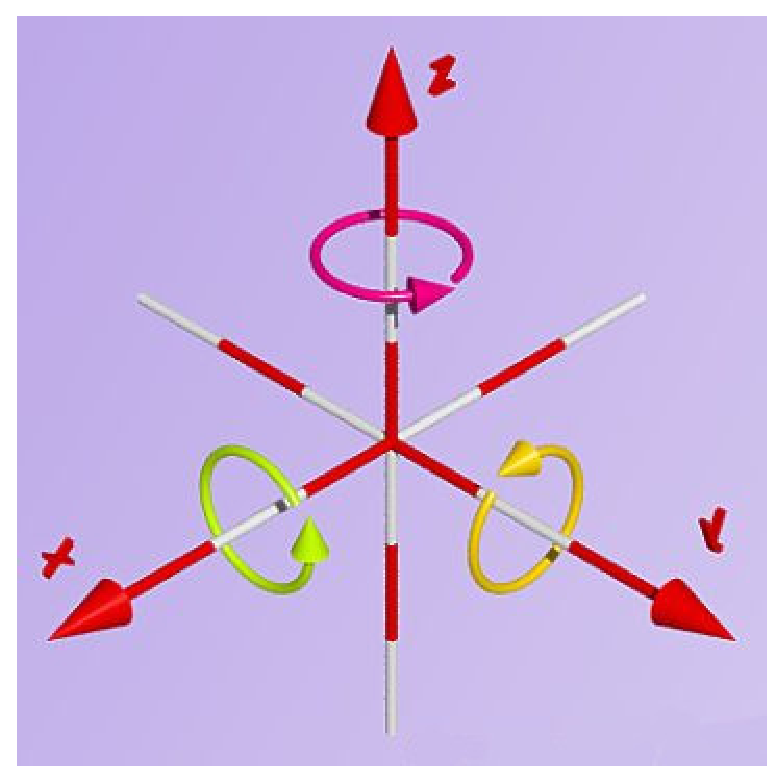
\includegraphics[width=0.4\textwidth]{gfx/axesRight.eps}}
  \caption{Left Handed Coordinate System and Right Handed Coordinate System}
  \label{fig:frames}
\end{figure}

By default \acrshort{povray} use a positive x value in the \inlinecode{POV}{right} vector. This means that the right side of the screen is aligned with the +x-direction. By using a negative x value in the \inlinecode{POV}{right} vector instead the right side of the screen will be aligned to the -x-direction, and the coordinate system will be right handed. Doing only that however left us having the y axis as the one pointing upward and the z axis as the one point in the direction which goes outside the screen.
To have a more comfortable reference frame, aligned with the \acrshort{gci} reference frame introduced in section \ref{sec:refereceFrames}, we can flip y and z axis by overriding the \inlinecode{POV}{sky} vector. By default, in fact, \acrshort{povray} uses \inlinecode{POV}{<0,1,0>} as \inlinecode{POV}{sky} vector. By redefining it as \inlinecode{POV}{<0,0,1>}  \acrshort{povray} will roll the camera until the top of the camera is in line with the \inlinecode{POV}{sky} vector, giving us the desired reference frame.

\begin{figure}[htbp]
  \centering
  \subfloat[\acrshort{povray} standard coordinate system]{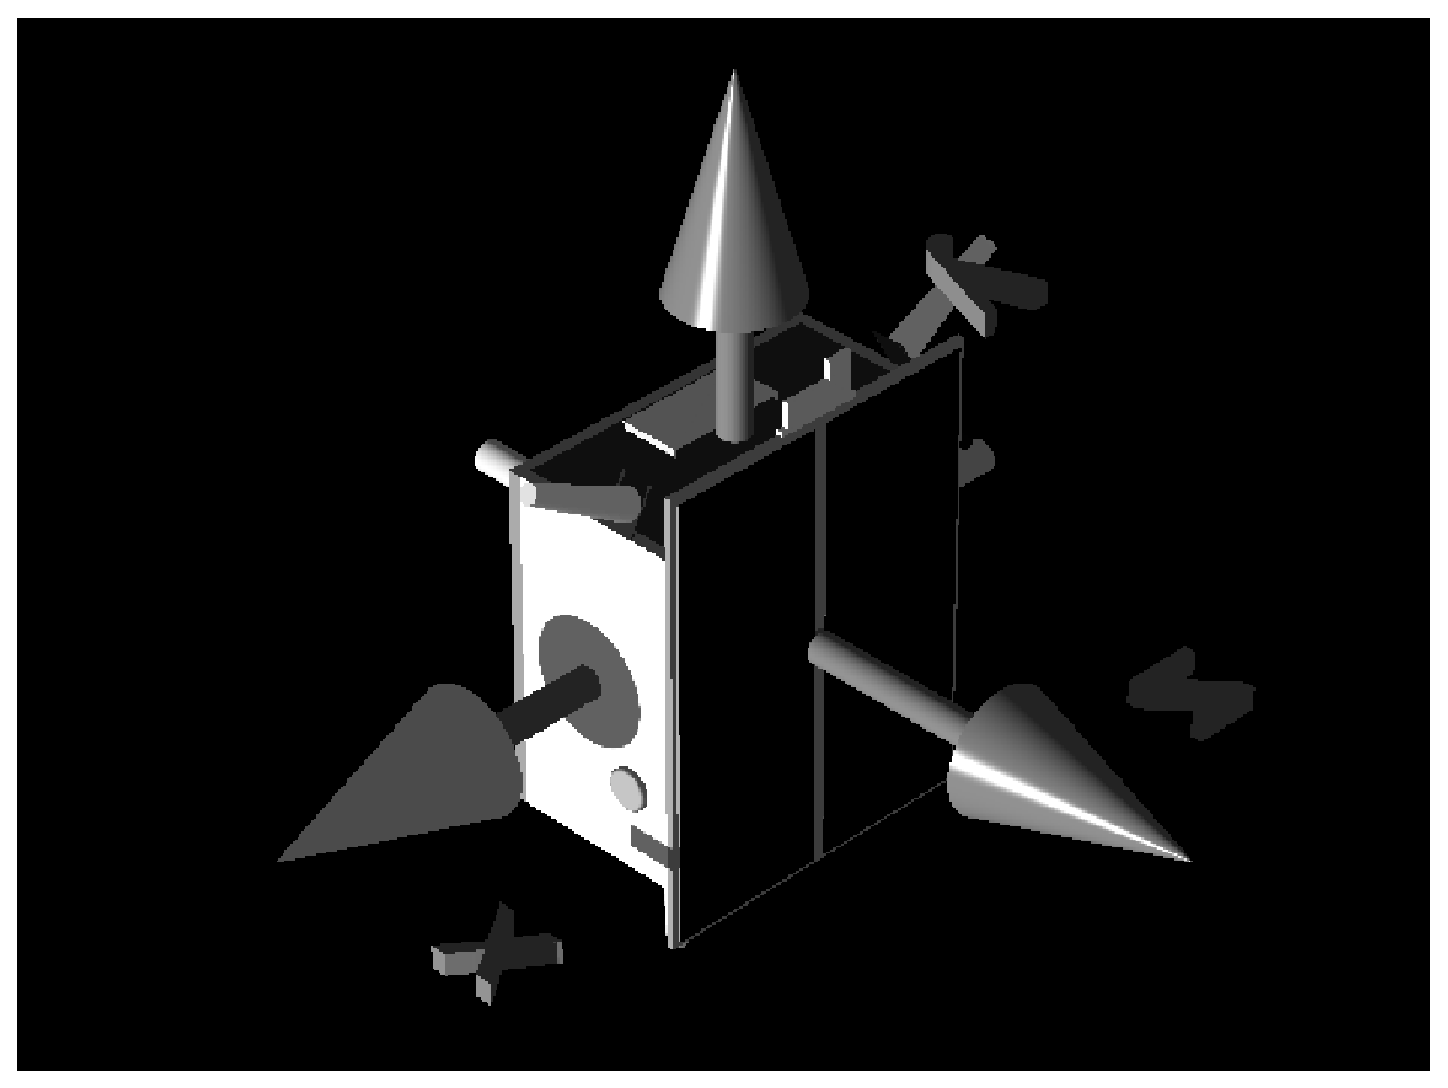
\includegraphics[width=0.47\textwidth]{gfx/tangoAxesNormal.eps}}
  \qquad
  \subfloat[Result after imposing negative x to the \inlinecode{POV}{right} vector ]{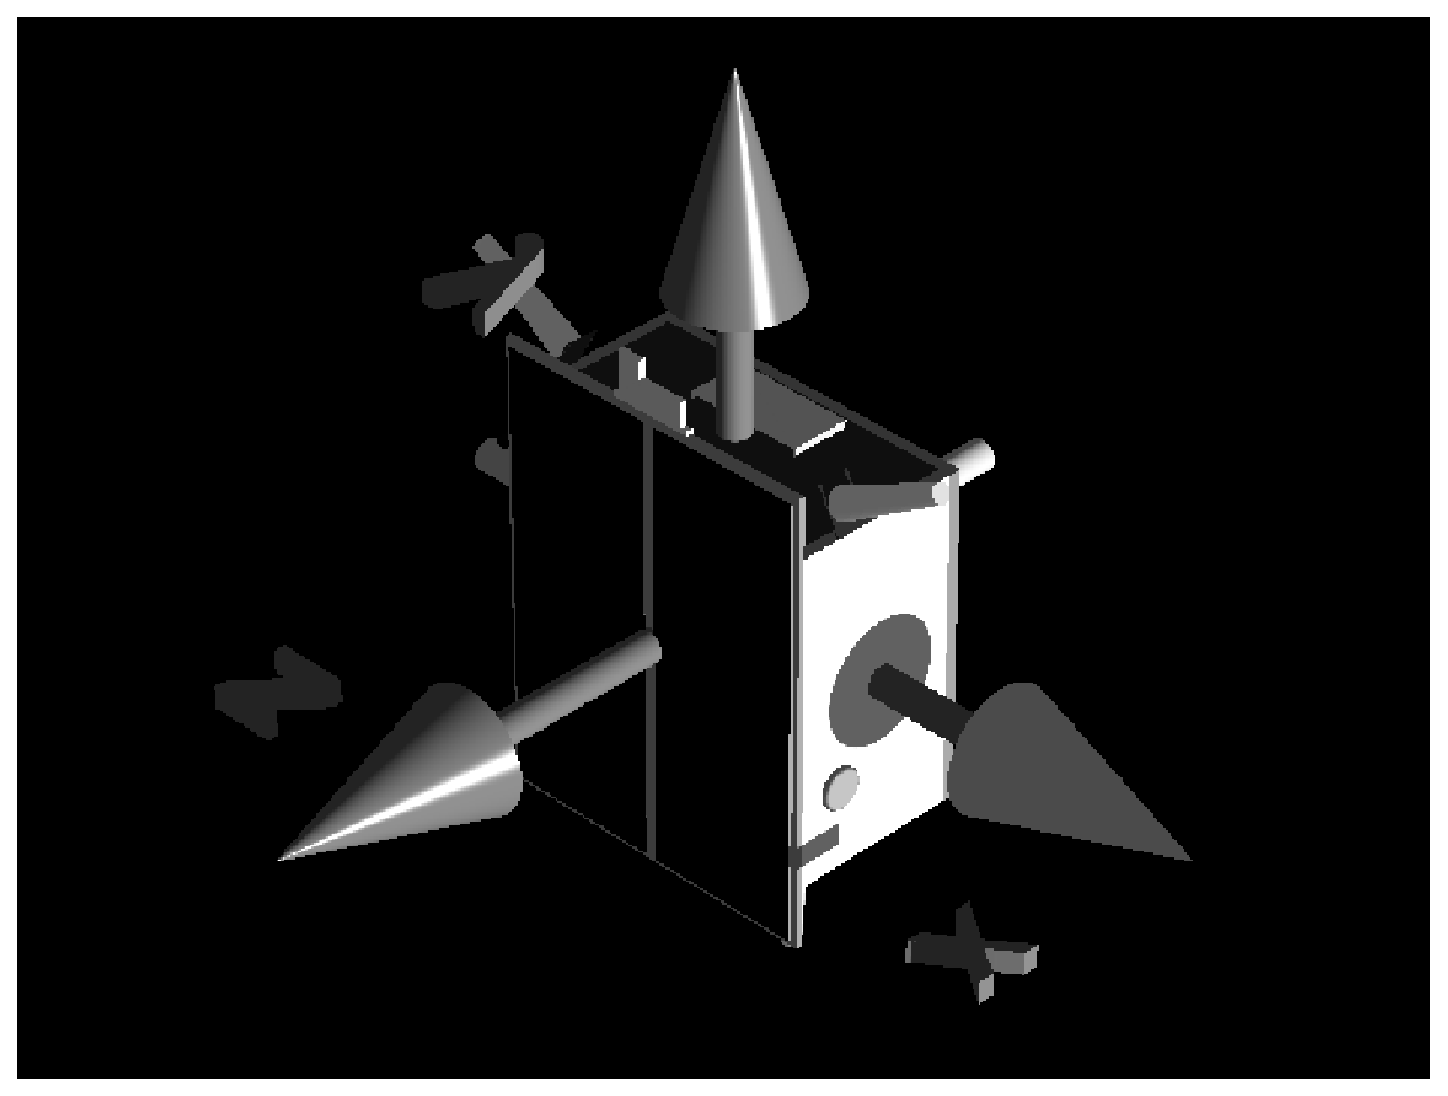
\includegraphics[width=0.47\textwidth]{gfx/tangoAxesAfterRight.eps}}
  \qquad
  \subfloat[Result after imposing \inlinecode{POV}{<0,0,1>} to the \inlinecode{POV}{sky} vector]{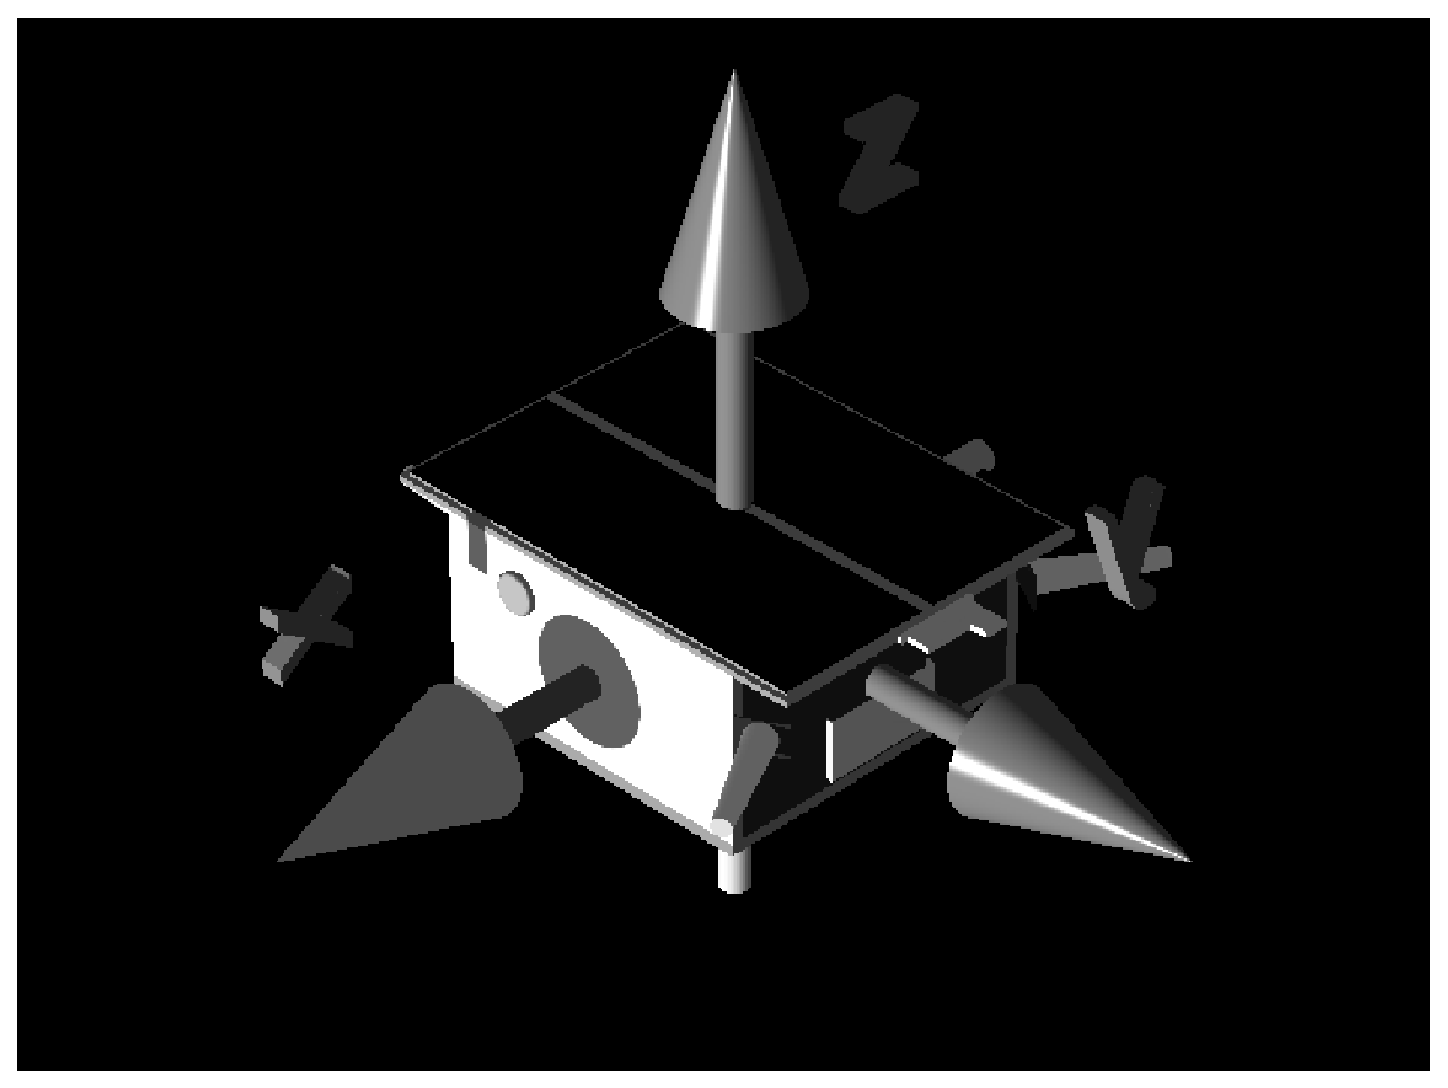
\includegraphics[width=0.47\textwidth]{gfx/tangoAxesSky.eps}}
  \caption{Reference Frame Rotations}
  \label{fig:framesComparison}
\end{figure}

In order to rightly simulate a real camera, the \acrshort{povray} camera aperture angle has been computed by assuming the intrinsic properties of a real camera, a Point Grey Grasshopper 3, equipped with a Xenoplan 1.9/17 mm lens, which is the same camera used to capture the real images of the SPEED data-set \cite{DBLP:journals/corr/abs-1911-02050}.

\begin{table}[htbp]
  \centering
  \begin{tabular}{ccc}
    \hline
    \hline
    Parameter & Description                 & Value             \\
    \hline
    $N_u$     & Number of horizontal pixels & 1920              \\
    \hline
    $N_v$     & Number of vertical pixels   & 1200              \\
    \hline
    $f_x$     & Horizontal focal length     & \SI{17.6}{\mm}    \\
    \hline
    $f_y$     & Vertical focal length       & \SI{17.6}{\mm}    \\
    \hline
    $d_u$     & Horizontal pixel length     & \SI{5.86e-3}{\mm} \\
    \hline
    $d_v$     & Vertical pixel length       & \SI{5.86e-3}{\mm} \\
    \hline
    \hline
  \end{tabular}
  \caption{Parameters of the camera used to capture the SPEED images \cite{DBLP:journals/corr/abs-1911-02050}}
  \label{tab:SPEEDCameraParameters}
\end{table}

By assuming a square \acrshort{ccd} sensor with square pixels we can obtain:

\begin{equation}
  A. R. = \frac{N_u}{N_v} \,,
\end{equation}

\begin{equation}
  CCD_{size} = d_u \cdot N_u \,,
\end{equation}

\begin{equation}
  \alpha = 2 \cdot \arctan{\left( \frac{CCD_{size}}{2 \cdot f_x} \right)} \,,
\end{equation}

where $A.R.$ is the Aspect Ratio of the picture, which is passed as first component \inlinecode{POV}{right} vector (with the negative sign, as described before), and $\alpha$ is the aperture angle which will be input in \acrshort{povray}.
Using the parameters detailed in table \ref{tab:SPEEDCameraParameters} we can compute:
\begin{itemize}
  \item \gls{ar} = $1.6$;
  \item \gls{alpha} = $35.4 ^{\circ}$.
\end{itemize}

\begin{figure}[htbp]
  \centering
  
\includegraphics[width=0.82\textwidth]{gfx/tangoNoNoise.eps}
  \caption{Tango \acrshort{sc} rendered using table \ref{tab:SPEEDCameraParameters} parameters}
  \label{fig:tangoNoNoise}
\end{figure}

\paragraph{Camera Attitude}\mbox{}\\
Being able to correctly know the imposed camera attitude at the moment of image generation is of crucial importance, especially when developing images to test pose determination algorithms.
Using the \inlinecode{POV}{look_at} keyword we specify the direction of the camera's boresight axis (so, in practice, where the camera is looking at, as the keyword itself suggest). Therfore, by imposing the \inlinecode{POV}{look_at} vector, we are implicitly imposing the camera attitude with respect to what is looking at. For what concerns this work, it is assumed that the camera always looks at the center of the target \acrshort{sc}.
By imposing \inlinecode{POV}{sky} and \inlinecode{POV}{right} vectors we impose the initial direction which \acrshort{povray} uses for orienting the camera.
By imposing the \inlinecode{POV}{look_at} vector \acrshort{povray} will first roll the camera until the top of the camera is in line with the sky vector. Then it uses the \inlinecode{POV}{sky} vector as the axis of rotation left or right and then to tilt up or down in line with the \inlinecode{POV}{sky} until until it lines up with the \inlinecode{POV}{look_at} point. Then tilts straight up or down until the \inlinecode{POV}{look_at} point is met exactly.

\begin{figure}[htbp]
  \centering
  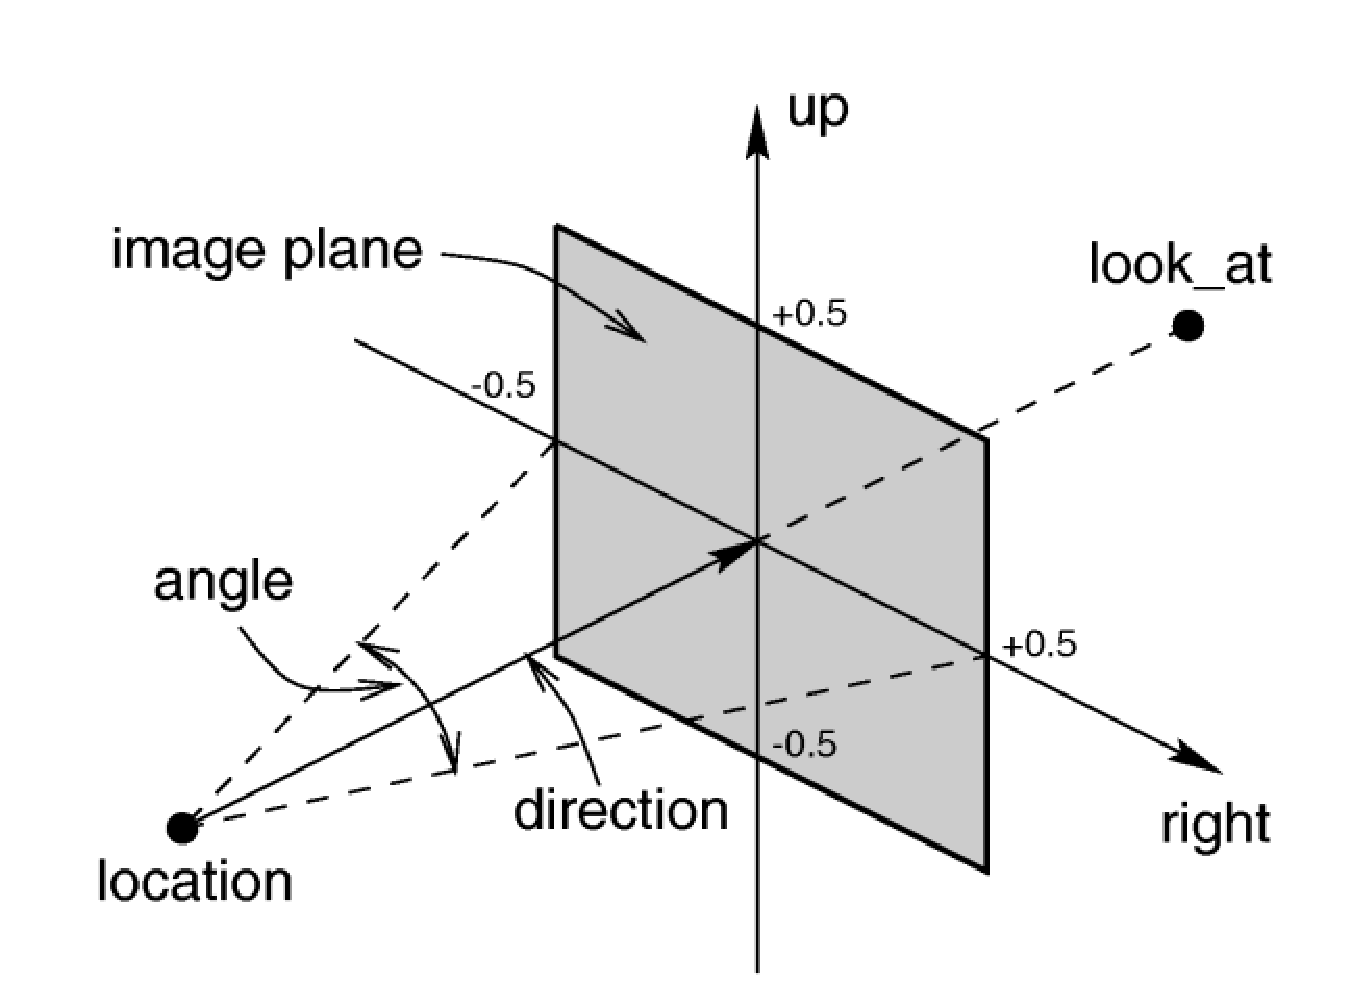
\includegraphics[width=0.82\textwidth]{gfx/perspcam.eps}
  \caption{\acrshort{povray} default perspective camera}
  \label{fig:perspcam}
\end{figure}

So, by knowing how \acrshort{povray} rotates the camera to point to the the \inlinecode{POV}{look_at} point, we can compute the actual attitude matrix of the camera with respect to the \acrshort{gci} frame\footnote{It is reminded to the reader that the \acrshort{gci} reference frame and the \acrshort{povray}'s world frame are aligned by design} exploiting simple linear algebra rules:

\begin{itemize}
  \item the z-direction, which is the one going straight out from the camera, can be computed by simply making the difference between the \inlinecode{POV}{look_at} vector and the camera \inlinecode{POV}{location} vector;
  \item the x direction, the one going right on the image plane, can be found by the cross product between the z-direction and the \inlinecode{POV}{sky} vector;
  \item the y direction, which is the one going downward in the image plane, can be found by performing the cross product between the z-direction and y-direction.
\end{itemize}

So, doing the needful math it is possible to write:

\begin{equation}
  \mathbf{\hat{z}} = \frac{\text{\inlinecode{POV}{look_at}} - \text{\inlinecode{POV}{location}}}{\norm{\text{\inlinecode{POV}{look_at}} - \text{\inlinecode{POV}{location}}}} \,,
\end{equation}

\begin{equation}
  \mathbf{\hat{x}} = \frac{\mathbf{\hat{z}} \wedge \text{\inlinecode{POV}{sky}}}{\norm{\mathbf{\hat{z}} \wedge \text{\inlinecode{POV}{sky}}}} \,,
\end{equation}

\begin{equation}
  \mathbf{\hat{y}} = \frac{\mathbf{\hat{z}} \wedge \mathbf{\hat{x}}}{\norm{\mathbf{\hat{z}} \wedge \mathbf{\hat{x}}}} \,.
\end{equation}

Knowing the versors which define the reference frame, the attitude of the camera with respect to the inertial \acrshort{povray} frame, \gls{A_CN}, can be simply defined as :

\begin{equation}
  \mathbf{{A_{CN}}} \triangleq [\mathbf{\hat{x}}, \mathbf{\hat{y}} \,. \mathbf{\hat{z}}]
\end{equation}

At this point, the imposed ground truth pose (\gls{A_TC}, \gls{t_c}) of the camera with respect to the \acrshort{sc} is completely defined by:

\begin{equation}
  \mathbf{{A_{TC}}} = \mathbf{{A_{CN}}} \mathbf{{A^T_{TN}}} \,,
\end{equation}

\begin{equation}
  \mathbf{t_C} = - (\text{\inlinecode{POV}{look_at}} - \text{\inlinecode{POV}{location}}) \mathbf{{A^T_{TN}}} \,.
\end{equation}

\subsection{Noise modeling}\label{subsection:addingthenoise}
Finally, for augmenting the "realness" of an image generated though \acrshort{povray}, the image needs to be post-processed using MATLAB.
The image so is input in MATLAB and two different noises are applied through the \inlinecode{MATLAB}{imnoise} command : speckle noise ($\sigma^2 = 0.004$) and Gaussian white noise ($\sigma^2 = 0.003$).
The final result can be seen in figure \ref{fig:comparisonNoise}.

\begin{figure}[htbp]
  \centering
  \subfloat[Image without noise added]{
\includegraphics[width=0.47\textwidth]{gfx/tangoNoNoise.eps}}
  \qquad
  \subfloat[Image wit speckle and Gaussian white noise]{\includegraphics[width=0.47\textwidth]{gfx/tangoNoise.eps}}
  \caption{Comparison between image without noise and image with speckle and Gaussian white noise}
  \label{fig:comparisonNoise}
\end{figure}

\section{MATLAB integration}
Since it would be highly unpractical to hand edit every time all the parameters to render the \acrshort{sc} in different position and attitudes as well as Earth's different rotations, a MATLAB toolbox has been developed which allows the user to automatically generate .pov \acrshort{sdl} files, and it renders them trough \acrshort{povray} automatically.
The implemented toolbox takes as input \gls{N_u}, \gls{N_v}, \gls{fx}, \gls{fy}, \gls{d_u}, \gls{d_v} to compute intrinsic camera parameters to set \acrshort{povray} camera.
Then, it offers the user the possibility to generate a sequence of random attitudes \cite{Arvo92}, given the orbital parameters of a reference orbit. If inertial properties of the target \acrshort{sc} are available, instead, it can compute the full uncontrolled dynamics (so to speak, the dynamics of the \acrshort{sc} when only subjected to the disturbances torques acting on the reference orbit) of the \acrshort{sc} trough a Simulink model at each time instant. For the interested reader, details about how the Space environment has been modeled in Simulink are given in \ref{app:first-appendix}.
For each time instant for which the attitudes of the target \acrshort{sc} have been computed, the relative position of the camera with respect to the target \acrshort{sc} is computed by selecting a random point inside a sphere having a \SI{20}{\m} radius centered in the target position, and the imposed pose is computed. A random Earth's rotation is computed as well.
All the properties of the scene are stored in a custom .att file, which can be passed in a second time to retrieve the absolute position and orientation of both the camera and the target \acrshort{sc} and their pose.
A .pov \acrshort{sdl} file is written for each time instant for which the attitudes of the target \acrshort{sc} have been computed and \acrshort{povray} is called to render each image in the background, from within MATLAB. Rightly after an image has been rendered, it is post-processed by MATLAB in order to add the noise, as described in \ref{subsection:addingthenoise}.

\section{Conclusions}
It must be noted by the reader, that a patched \acrshort{povray} version is required in order to correctly replicate what has been done in this project, as stated in the first lines of section \ref{sec:3dmodel}. At the beginning of this project it has been decided that by design, 1 unit in the \acrshort{povray} world is exactly equal to \SI{1}{\km} to ease the modeling of the solar system. Thus, the Earth is placed at the origin of the \acrshort{povray} world (consistently with the \acrshort{gci} frame)and it has a \SI{6378}{\km} radius, and the light source, the Sun, is placed \SI{1.4723e8}{\km} far from the Earth, and has a radius of \SI{696340}{\km}.
The \acrshort{sc} instead is placed on an orbit characterized by the orbital parameters specified in table \ref{tab:orbitalParameters}. The inertial properties of the target instead are computed by assuming a mass of \SI{50}{\kg} and using the dimension given in \ref{sec:3dmodel}.

\begin{table}[htbp]
  \centering
  \begin{tabular}{ccc}
    \hline
    \hline
    Orbital Parameters & Symbol   & Values         \\
    \hline
    Apogee             & $r_a$    & \SI{7178}{\km} \\
    \hline
    Perigee            & $r_p$    & \SI{7101}{\km} \\
    \hline
    Semimajor axis     & $a$      & \SI{7133}{\km} \\
    \hline
    Inclination        & $i$      & \ang{98.28}    \\
    \hline
    Pericenter anomaly & $\omega$ & \ang{0}        \\
    \hline
    True anomaly       & $\theta$ & \ang{0}        \\
    \hline
    Eccentricity       & $e$      & \ang{0.0045}   \\
    \hline
    \hline
  \end{tabular}
  \caption{Parameters used to generate the reference orbit \cite{prismaOrbitParameters}}
  \label{tab:orbitalParameters}
\end{table}

So, what is being represented is a scene having an extremely small object (the \acrshort{sc}) in front of a giant object {the Earth}, which is impacted by light which is generated from a very far distance (the Sun). Due to the exquisite peculiarity of this kind of scene, in some corner cases a "bounding issue" can be triggered, causing the \acrshort{sc} to be only partially redendered in the scene, or, in worst case scenario, not being rendered at all. Directly citing the \acrshort{povray} documentation, in order to speed up the ray-object intersection tests \acrshort{povray} uses a variety of spatial sub-division systems. The primary system uses a hierarchy of nested bounding boxes. This system compartmentalizes all finite objects in a scene into invisible rectangular boxes that are arranged in a tree-like hierarchy. Before testing the objects within the bounding boxes the tree is descended and only those objects are tested whose bounds are hit by a ray. This can greatly improve rendering speed. However, during the development of this project turned out that \acrshort{povray} automatic bounding is not perfect. There are situations where a perfect automatic bounding is very hard to calculate, like the one faced in this project. Unfortunately, \acrshort{povray} developers removed the possibility of turning off bounding control in \acrshort{povray}, thus it is necessary to compile a patched \acrshort{povray} version which introduces back the command line switch \textbf{-MB} which allows the user to turn off bounding control. According to the GPL license \acrshort{povray} is shipped with, the patch has been made freely available \footnote{\url{https://github.com/fcuzzocrea/povray/commit/2aecdfb20eef3ed3b6a5698392a9c91fa3f1afcd}}.
The output of the toolbox which has been described trough this chapter can be observed in figure \ref{fig:finalResult}.

\begin{figure}[htbp]
  \centering
  \subfloat[]{\includegraphics[width=0.47\textwidth]{gfx/tango/tango_14.eps}}
  \qquad
  \subfloat[]{\includegraphics[width=0.47\textwidth]{gfx/tango/tango_15.eps}}
  \qquad
  \subfloat[]{\includegraphics[width=0.47\textwidth]{gfx/tango/tango_31.eps}}
  \qquad
  \subfloat[]{\includegraphics[width=0.47\textwidth]{gfx/tango/tango_60.eps}}
  \qquad
  \subfloat[]{\includegraphics[width=0.47\textwidth]{gfx/tango/tango_259.eps}}
  \qquad
  \subfloat[]{\includegraphics[width=0.47\textwidth]{gfx/tango/tango_268.eps}}
  \qquad
  \subfloat[]{\includegraphics[width=0.47\textwidth]{gfx/tango/tango_228.eps}}
  \qquad
  \subfloat[]{\includegraphics[width=0.47\textwidth]{gfx/tango/tango_258.eps}}
  \qquad
  \caption{Final result}
  \label{fig:finalResult}
\end{figure}
\cleardoublepage{}
\chapter{The SVD architecture for pose initialization\label{chap:third-chapter}}
\begin{quotation}
  {\footnotesize
    \noindent{\emph{``Prediction is very difficult, especially if it's about the future.''\\}
    }
    \begin{flushright}
      Niels Bohr
    \end{flushright}
  }
\end{quotation}
\vspace{0.5cm}

Performing a robust pose initialization from a \acrshort{2d} image captured by a monocular camera in space is a very though task, particularly due to the fact that illumination conditions in space may vary during a single orbit, and therefore may cause inaccurate and unreliable features detection. Moreover, the Earth presence in the background introduces a major complexity into distinguishing the target \acrshort{sc} shape from the Earth surface. The \acrshort{svd} pose initialization architecture aims at solving the problem of pose initialization by employing a single \acrshort{2d} image taken by a monocular camera. In this chapter first the reader will be proposed with a brief \acrfull{cv} mathematical concerning some common \acrfull{cv} models and problems. After that, a detailed description of the \acrshort{svd} architecture implementation which has been carried out in this work will be given.

\section{Mathematical Preliminaries}

\subsection{Pinhole Camera Model}\label{subsection:pinhole}
The pinhole camera model is camera model which is widely used in \acrfull{cv}. Despite being a relatively simple model, it is still accurate enough for the vast majority of applications. The pinhole camera model is used to describe the mathematical relationship which exists between the coordinates of a point in the \acrshort{3d} world and its projection onto the image plane. In the pinhole camera model, the light passes trough a single point, the camera center, before being projected onto the image plane, and no lenses are used to focus light, so geometrical distortions or blurring are not modeled in the pinhole camera model.

\begin{figure}[htbp]
  \centering
  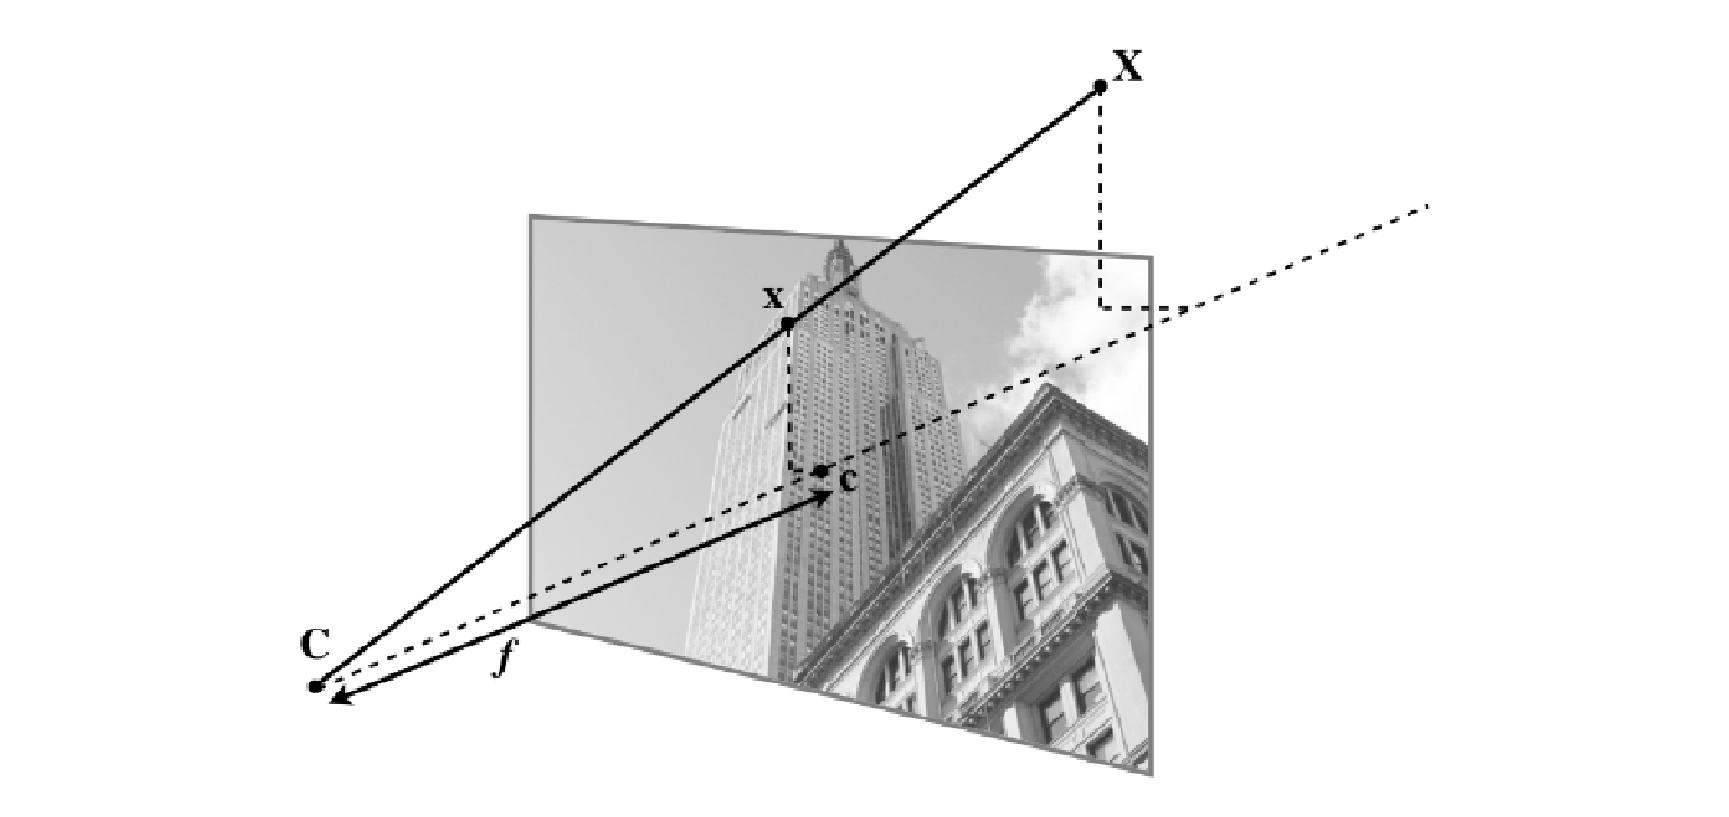
\includegraphics[width=0.85\textwidth]{gfx/pinholeCamera.eps}
  \caption{The pin-hole camera model \cite{solem2012programming}}
  \label{fig:pinholeCamera}
\end{figure}

By referring to \ref{fig:pinholeCamera}, a \acrshort{3d} point $\mathbf{X}$ is projected to an image point $\mathbf{x}$ (both expressed in homogeneous coordinates) as :

\begin{equation*}
  \lambda\mathbf{x}=P\mathbf{X} \,,
\end{equation*}

where $P$ is a 3-by-4 matrix called camera matrix and $\lambda$ is a scalar number representing the inverse depth of the \acrshort{3d} point. As a result, the \acrshort{3d} point $\mathbf{X}$ is characterized by four elements, $X = [X, Y , Z, W ]$ in homogeneous coordinates.
Generally, the camera matrix $P$ can be decomposed as :

\begin{equation*}
  P = K[R \ | \ \mathbf{t}] \,,
\end{equation*}

where $R$ is the rotation matrix which describes the orientation of the camera, $\mathbf{t}$ is a \acrshort{3d} translation vector which describes the position of the camera center and $K$ is the intrinsic camera calibration matrix.
The camera calibration matrix basically describes the projection properties of the camera and can be written as :

\begin{equation*}
  K = \begin{bmatrix}
    \alpha f & s & c_x \\
    0        & f & c_y \\
    0        & 0 & 1
  \end{bmatrix} \,,
\end{equation*}

where $\alpha$ is the aspect ratio of the sensor's pixels, $f$ is the focal length, $s$ is the skew and $c_x$, $c_y$ are the coordinates of the optical center (or also called the principal point) of the image. Usually the principal point of the image can be approximated with half the height and half the width of the image. The skew is used only if the pixel array in the sensor is skewed. In most cases is safe to assume $s = 0$.
By defining :

\begin{equation*}
  f_x = \alpha f_y
\end{equation*}

and by neglecting $s$ we can write the calibration matrix in the most common form :

\begin{equation*}
  K = \begin{bmatrix}
    f_x & 0   & c_x \\
    0   & f_y & c_y \\
    0   & 0   & 1
  \end{bmatrix} \,,
\end{equation*}

If we make the assumption of square pixel, then $\alpha = 1 $ and $ f_x = f_y = f$, and so we can write the camera calibration matrix as :

\begin{equation*}
  K = \begin{bmatrix}
    f & 0 & c_x \\
    0 & f & c_y \\
    0 & 0 & 1
  \end{bmatrix} \,.
\end{equation*}

More information about camera model and camera calibration matrix can be found in \cite{10.5555/861369} and \cite{Pollefeys2004}.

\subsection{Image derivatives}\label{sec:imagegradient}
For a grayscale image, the image intensity changes over the image itself can be described by using the $x$ and $y$ derivatives, $I_x$ and $I_y$ of the graylevel image $I$.
Once defined the image derivatives, it is possible to define another quantity, the image gradient, which is the vector:

\begin{equation*}
  |\nabla I| = \sqrt{I_x^2 + I_y^2} \,,
\end{equation*}

which describes how strong the image intensity change. Image derivatives can be computed using a discrete approximations, which are implemented as convolutions:

\begin{equation*}
  I_x = I * D_x \ \ \,, \ \ I_y = I * D_y \,,
\end{equation*}

where $D_x$, $D_y$ are the kernel of the derivative and $*$ is the \acrshort{2d} convolutional operation. Two common choices for $D_x$, $D_y$ are either the so called Prewitt filters :

\begin{equation*}
  D_x = \begin{bmatrix}
    -1 & 0 & 1 \\
    -1 & 0 & 1 \\
    -1 & 0 & 1
  \end{bmatrix} \ \ \,,  \ \
  D_y = \begin{bmatrix}
    -1 & -1 & -1 \\
    0  & 0  & 0  \\
    1  & 1  & 1
  \end{bmatrix}\,,
\end{equation*}

or the so called Sobel filters:

\begin{equation*}
  D_x = \begin{bmatrix}
    -1 & 0 & 1 \\
    -2 & 0 & 2 \\
    -1 & 0 & 1
  \end{bmatrix} \ \ \,,  \ \
  D_y = \begin{bmatrix}
    -1 & -2 & -1 \\
    0  & 0  & 0  \\
    1  & 2  & 1
  \end{bmatrix}\,,
\end{equation*}

\subsection{The Hough Transform}\label{sec:hough}
The Hough transform is a method often used in \acrfull{cv} for finding shapes in images. It wors by using a voting procedure in the parameters space of the shapes. The most common use of the Hough transform is to find lines in images.
Consider the straight line equation, in its polar form,

\begin{equation*}
  \rho = x \cos{\theta} + y \sin{\theta} \,,
\end{equation*}

\begin{figure}[htbp]
  \centering
  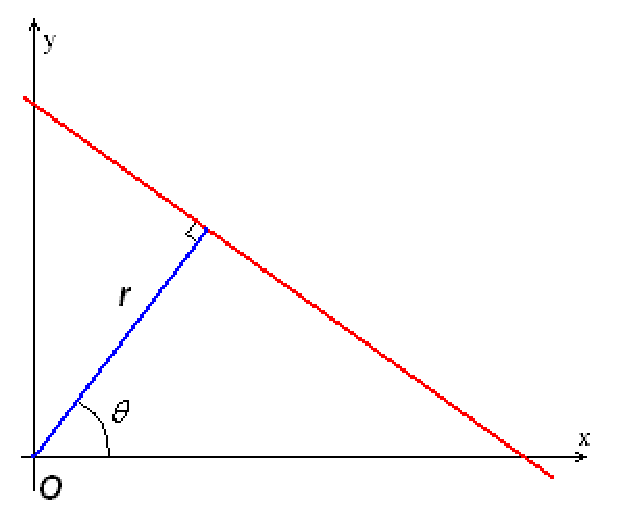
\includegraphics[width=0.45\textwidth]{gfx/R_theta_line.eps}
  \caption{Polar representation of a straight line \cite{pichough}}
  \label{fig:linePolar}
\end{figure}

where $\rho$ obviously is the distance from the origin of the reference system to the closest point on the straight line, while $\theta$ is the angle between the x axis and the line connecting the origin with that closest point.
The linear Hough transform algorithm estimates the two parameters that define the straight line. The transform space has two dimensions, and any point in the transform space is used as an accumulator (a bi-dimensional vector) to detect a line described by the aforementioned polar equation of the straight line. Every point in the detected edges in the image contributes to the accumulators. Generally, the dimension of the accumulator is equal to the number of unknown parameters, which in this case are two, $\rho$ and $\theta$. For each pixel and is neighborhood, the algorithm which computes the Hough transform first try to detect if the specific pixel which is being analyzed lie on a line. If so, computes $\rho$ and $\theta$ of that line, and then look for the accumulator's bin that the parameters fall into, and increment the value of that bin.
By searching the boxes with highest values, typically by looking at local maxima in the accumulator space, it is possible to identify the the most likely lines. The final result of the Hough transform will be a \acrshort{2d} matrix, were one dimension will be represented by $\theta$ and the other one by $\rho$.
Each element of that matrix will have a value equal to the sum of the pixels that are positioned on the line represented by the parameters $\rho$, $\theta$. So the element with the highest value indicates the straight line that is most represented in the input image \cite{houghreport}. More information about the how the Hough transform works can be retrieved in \cite{10.1145/361237.361242} and \cite{osti_4746348}.

\subsection{Perspective-n-Point problem}
The \acrfull{pnp} point is the problem of determining the position and the orientation of a calibrated camera given its intrinsic parameters and a set of correspondences between a given set of \acrshort{3d} points and their respective \acrshort{2d} projections in the image \cite{10.1007/s11263-008-0152-6}.
The perspective projection for a standard pinhole camera that has been introduced in section \ref{subsection:pinhole} leads to the following equation (in homogeneous coordinates) for the model:

\begin{equation*}
  \lambda
  \begin{bmatrix}
    u \\
    v \\
    1 \\
  \end{bmatrix}
  =
  \begin{bmatrix}
    f & 0 & c_x \\
    0 & f & c_y \\
    0 & 0 & 1
  \end{bmatrix}
  \begin{bmatrix}
    r_{11} & r_{12} & r_{13} & t_1 \\
    r_{21} & r_{22} & r_{23} & t_2 \\
    r_{31} & r_{32} & r_{33} & t_3
  \end{bmatrix}
  \begin{bmatrix}
    x \\
    y \\
    z \\
    1 \\
  \end{bmatrix} \,,
\end{equation*}

were $r_{ij}$ and $t_i$ are the components of the rotation matrix and the translation vector which are being calculated, respectively.
Several methods exists for solving the \acrshort{pnp} problem, the two most common of which are the P3P method and the \textit{e}\acrshort{pnp} method. More information about their implementations can be found on  \cite{XiaoShanGao2003} \cite{Torr2000} and \cite{10.1007/s11263-008-0152-6}.

\section{Feature-based pose estimation implementation: the SVD algorithm}
The images generated  trough the toolbox presented in Chapter \ref{chap:second-chapter} will now be analyzed using the robust monocular vision-based pose initilization algorithm proposed by S. Sharma, J. Ventura and S. D'Amico in \cite{Sharma2018}.
As briefly explained in the introduction, the problem of pose initialization consists in computing the rotation matrix,\gls{A_TC} and the translation vector, \gls{t_c} that describes the transformation between the camera frame, $C$, and the target body frame, $B$. Given a generic image point, $p$ = $ [u,v]^T $, we can relate the corresponding $\mathbf{q_B}$ point of the \acrshort{3d} model by employing the standard pinhole camera model briefly reviewed in section \ref{subsection:pinhole}:

\begin{equation}
  \mathbf{r_C} = \left[x_C \quad  y_C \quad z_C\right]^T = \mathbf{A_{TC}} \; \mathbf{q_B} + \mathbf{t_C} \,,
  \label{eq:rc}
\end{equation}

\begin{equation}
  \mathbf{p} = \left[ \frac{x_C}{z_C} f_x + C_x , \frac{y_C}{z_C} f_y + C_y \right] \,,
  \label{eq:p}
\end{equation}

where \gls{fx} and \gls{fy} are the respectively the horizontal and the vertical focal length and $ \left[C_x, \ C_y \right]$ are the coordinates of the center of the image. Moreover, it is assumed - without loss of generality - that the direction $\mathit{C_3}$ of the camera frame is pointed along the boresight of the camera and the directions $\mathit{C_1}$ and $\mathit{C_2}$ are aligned with the image frame defined by $P = \left( \mathit{P_1}, \ \mathit{P_2} \right)$

\begin{figure}[htbp]
  \centering
  \includegraphics[width=0.72\textwidth]{gfx/poseProblem.eps}
  \caption{Schematic representation of the pose estimation problem using a monocular image \cite{Sharma2018}}
  \label{fig:theposeproblem}
\end{figure}

To be able to uniquely solve this set of equation are needed at least six correspondences between the image points and the model points \cite{10.1145/358669.358692}. The challenging part of the problem is to be able to correctly detect the most meaningful points in the \acrshort{2d} image. Usually this can be archived by employing edge detection techniques, such as the Canny edge detector \cite{10.1109/TPAMI.1986.4767851} followed by the Hough transform \cite{10.1145/361237.361242}. This approach however may be biased it applied dierctly to the image due to the fact that these algorithm are gradient based and are not able to correctly distinguish the foreground from the background and also requires the definition of numerous hyperparameters which are difficult to tune for broad applicability because the imaged scene and the illumination conditions are constantly changing throughout the orbit \cite{Sharma2018}.

\subsection{Architecture}
In \cite{Sharma2018} is proposed a novel architecture to solve the initial pose of a non cooperative client \acrshort{sc}, whose pipeline is depicted in figure \ref{fig:theposeproblem}.

\begin{figure}[htbp]
  \centering
  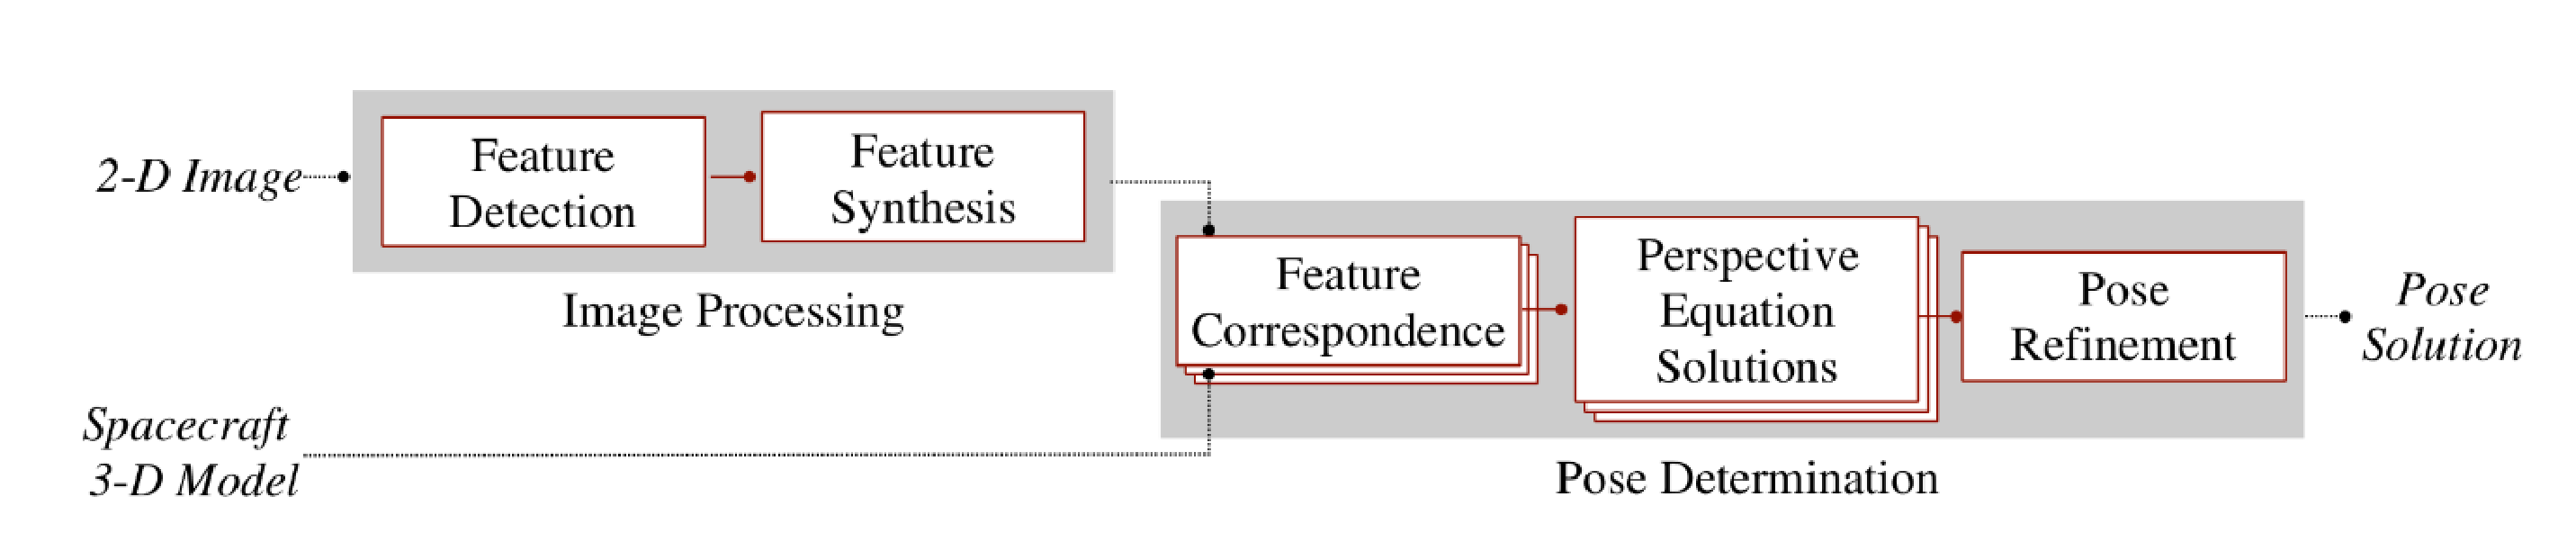
\includegraphics[width=0.85\textwidth]{gfx/SVDPipeline.eps}
  \caption{The \acrshort{svd} architecture for solving the pose estimation problem \cite{Sharma2018}}
  \label{fig:theposeproblem}
\end{figure}

Its key features are (directly citing \cite{Sharma2018})  :
\begin{itemize}
  \item the fusion of the \acrshort{wge} technique with the more traditional Sobel edge detector and the Hough algorithm to perform the feature detection;
  \item the use of feature synthesis to reduce the search space for feature correspondences between the features extracted from the images and the \acrshort{3d} model;
  \item the combination of the \textit{e}\acrshort{pnp} solver and the \acrfull{nr} method for the final pose determination.
\end{itemize}

As the reader can see from the schematic represented in figure \ref{fig:theposeproblem}, the pipeline is composed from two different subsystems:
\begin{itemize}
  \item the image processing subsystem, which receive as an input a \acrshort{2d} image, distinguishing the \acrshort{sc} from the image, extract its edge features and groups them into geometric groups;
\end{itemize} the pose determination subsystems, which acceps as input the previously feature groups detected by the image processing subsystem and the \acrshort{3d} model. It then pairs the \acrshort{2d} and \acrshort{3d} geometric groups to formulate multiple correspondence hypotesis. For each hypothesis formulated, the endpoints of the line segments forming the geometric groups are used to solve equation \eqref{eq:rc} and equation \eqref{eq:p}. The five best solution then are iteratively refined by employing the \acrshort{nr} method.

two are the most meaningful innovation the \acrshort{svd} architecture introduces:
\begin{itemize}
\item the usage of the \acrshort{wge} technique in order to distinguish the target \acrshort{sc} from the background and for enhancing the output of the edge detection procedure bu providing a robust identification of the small as well as large edges of the \acrshort{sc};
\item the usage of feature groups detected in the image and in the \acrshort{3d} model to solve the feature correspondence problem, which also allows the \acrshort{svd} architecture to be more computationally efficient.  
\end{itemize}

\subsection{Image processing subsystem}
The taks of the image processing subsystem is to extract the most meaningful features from the \acrshort{2d} image a of the target \acrshort{sc}. To effectively and rapidly detect the target \acrshort{sc} edges - even in presence of the Earth in the background - an hybrid image processing subsystem is proposed in \cite{Sharma2018}. 
By fusing together the \acrshort{wge} technique and classical state-of-the-art edge detection techniques the architecture proposed by \textit{Et al.} is capable to provide a robust and efficient identification of the rue edges of the \acrshort{sc}.
In particular, the \acrshort{wge} technique is able to identify the a \acrfull{roi} in a more accurate and robust way with respect to state-of-art techniques. The \acrshort{roi} is detection not only makes the entire subsystem robust against the background, but also allows an automated selection of the hyperparameters needed for the Hough transform, which will be used to detect both small and large features of the \acrshort{sc}, in contrast with state-of-the-art algorithms which rely on a single set of manually tuned hyperparameters.
The flow of the image processing subsystem is illustrated in figure \ref{fig:imageProcessingSubsystem}.

\begin{figure}[htbp]
  \centering
  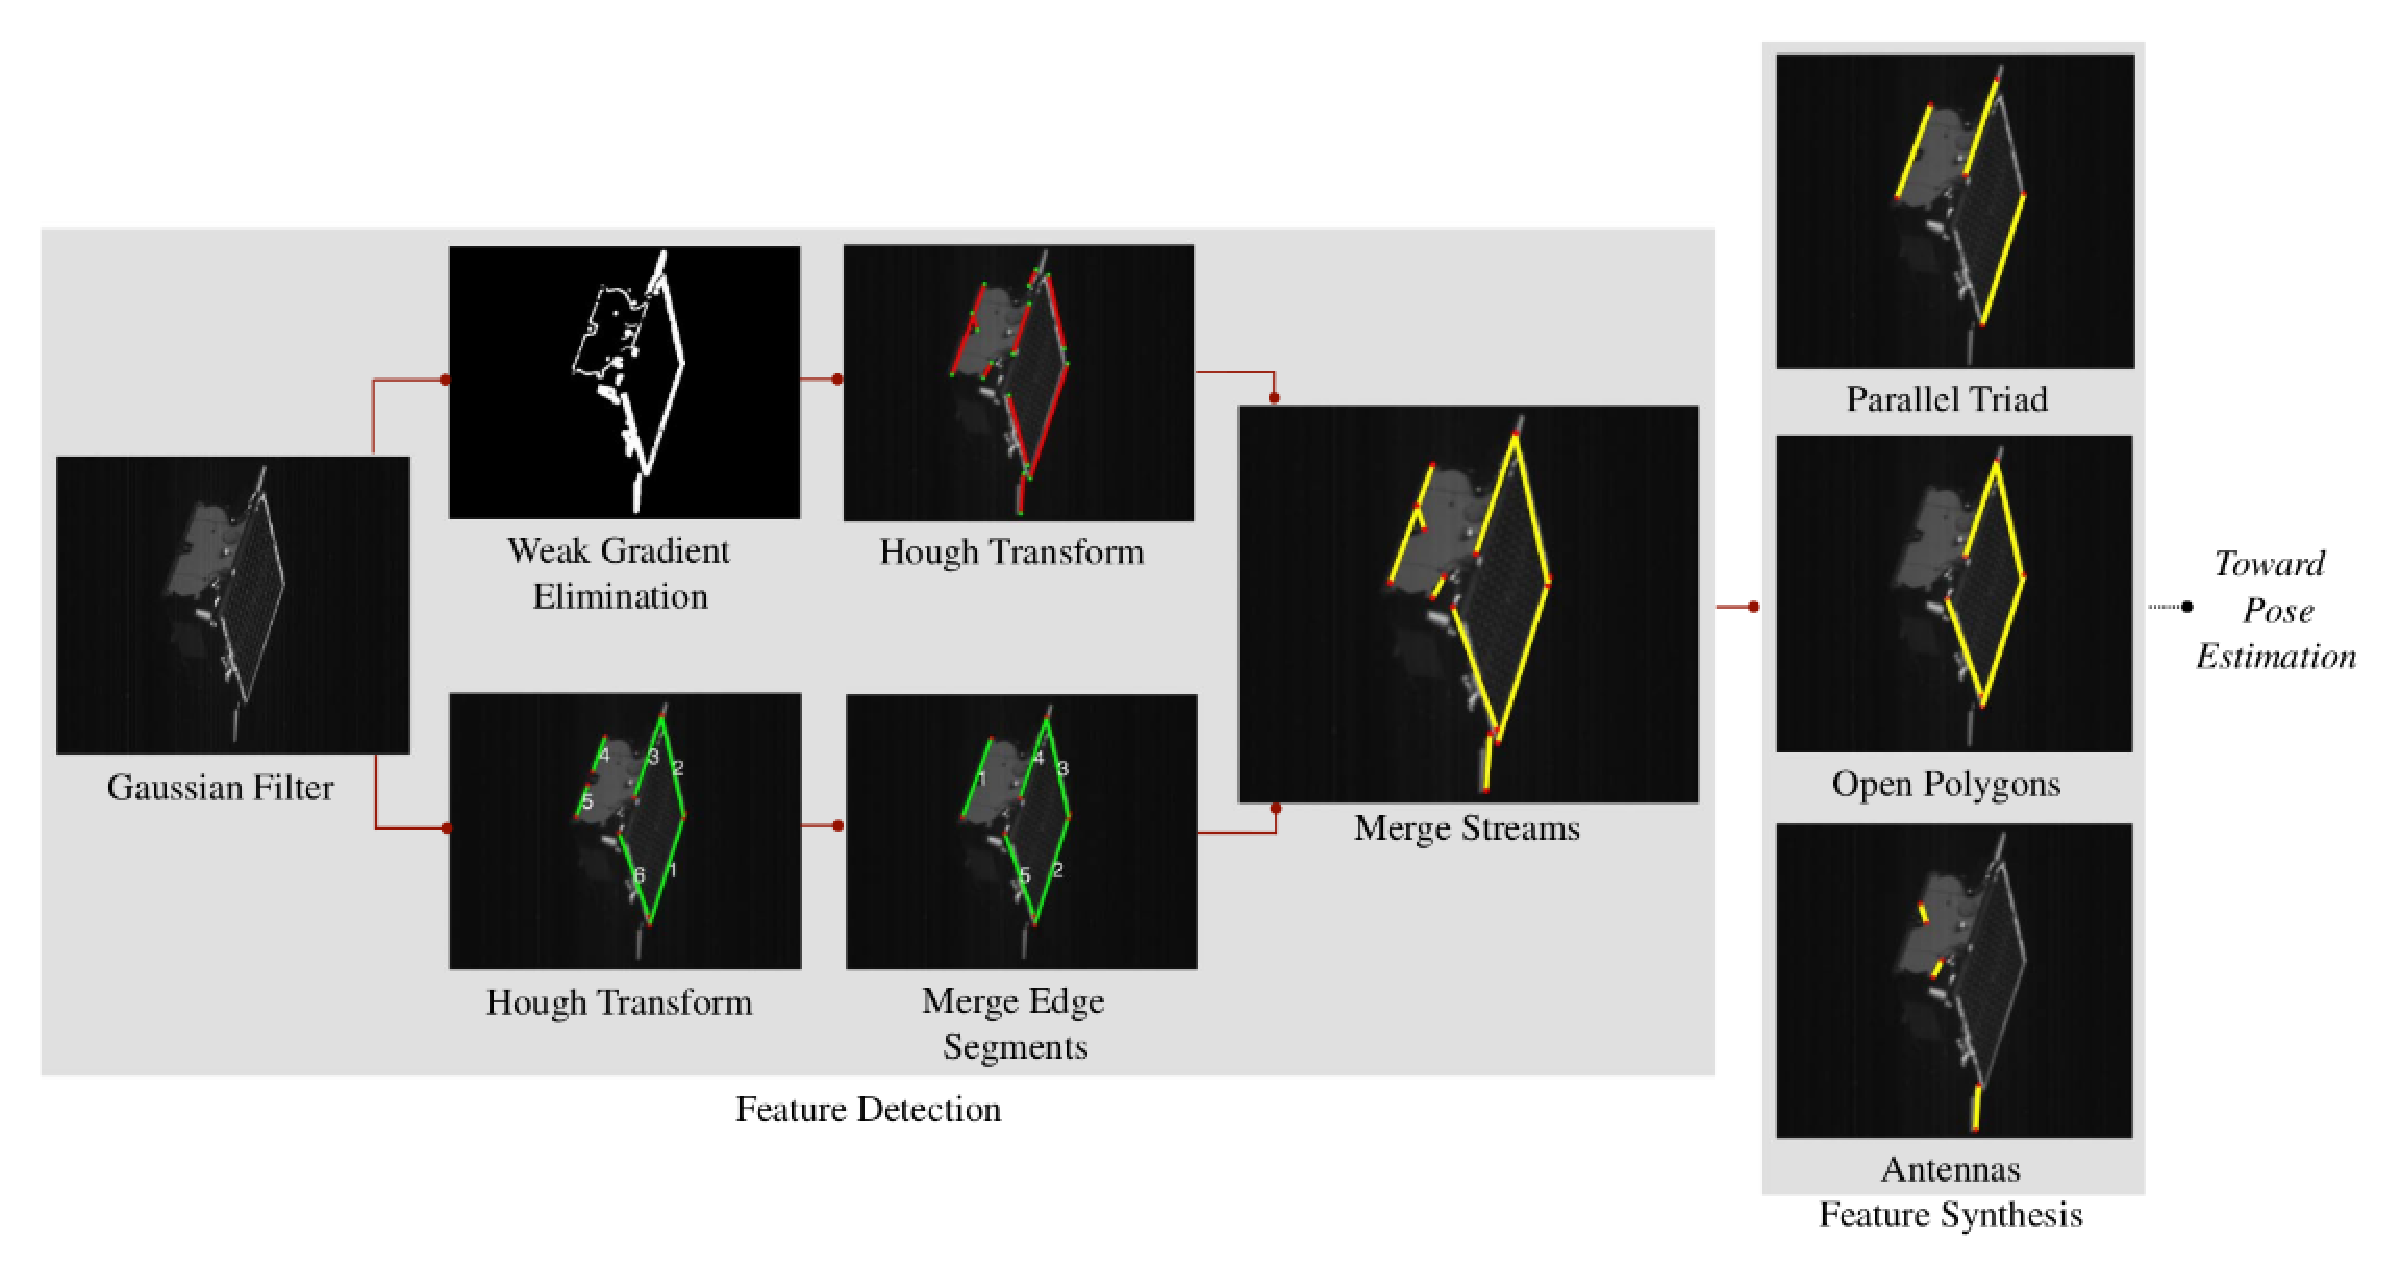
\includegraphics[width=0.85\textwidth]{gfx/imageProcessingSubsystem.eps}
  \caption{The image processing subsystem \cite{Sharma2018}}
  \label{fig:imageProcessingSubsystem}
\end{figure}

\subsubsection{Feature Detection}
The first sub-block of the pose estimation technique proposed in \cite{Sharma2018} is the feature detection subsystem, whose aim is to  identify, in the input image, a set of segments that corresponds to the true edges of the target \acrshort{sc}.
The raw input image - assumed to be rectified - is imported in MATLAB and is converted to the uint8 data type trough the command \inlinecode{MATLAB}{im2uint8} . After that, A Gaussian filter is applied in order to the decrease the magnitude of image noise. The Gaussian filtering can be carried out by using the MATLAB function \inlinecode{MATLAB}{imgaussfilt}, which let the user set the desired filtering depth. For what concerns this work, the images generated in chapter \ref{chap:second-chapter}, before being fed to the image processing subsystem have been filtered by using a standard deviation $\sigma_X = 1.15$. During this work, has been observed that the choice of the $\sigma_X$ value is very important for the success of the subsequent steps, as a wrong value can highly impact the effectiveness of the \acrshort{wge} technique. Once the image has been prefiltered, is fed as input to the \acrshort{wge} block, for the computation of the target's \acrshort{roi}. The first step consist in computing the magnitude of the image gradient, $|\nabla I|$,  using the Prewitt filter for computing the image gradient, as showed in section \ref{sec:imagegradient}.
The \acrshort{sc} can be detected in the image by observing that, under most illumination conditions, in correspondence of the target \acrshort{sc} edges the gradient variation is more pronounced with respect to the background, regardless of the fact that the background is empty or the Earth is behind.
Indeed, to detect the spacecraft, the gradient distribution is normalized using the MATLAB \inlinecode{MATLAB}{mat2gray} function, sorted into $100$ uniformly distributed bins and fitted by and exponential \acrfull{pdf}, described by the equation :

\begin{equation*}
  y = \frac{1}{\mu} e^{-\frac{x}{\mu}} \,.
\end{equation*}

By observing the result histogram, it is clearly possible to see that most of the gradient intensities are weak and corresponds to the feature in the background or on the spacecraft surface. The weak gradient pixel locations can be classified by tresholding the \acrshort{pdf} fit to the gradient histogram. The original authors suggest to use a value of $.0.99$ to treshold the \acrshort{pdf}, however, for what concerns this work, all the pixel which corresponds to a cumulative distribution inferior to $0.996$ are classified as weak and set to zero instead. Once the weak gradients are set to zero, only the most prominent features of the \acrshort{sc} are present in the image, as shown in figure \ref{fig:wgeSteps}.

\begin{figure}[htbp]
  \centering
  \subfloat[Original image]{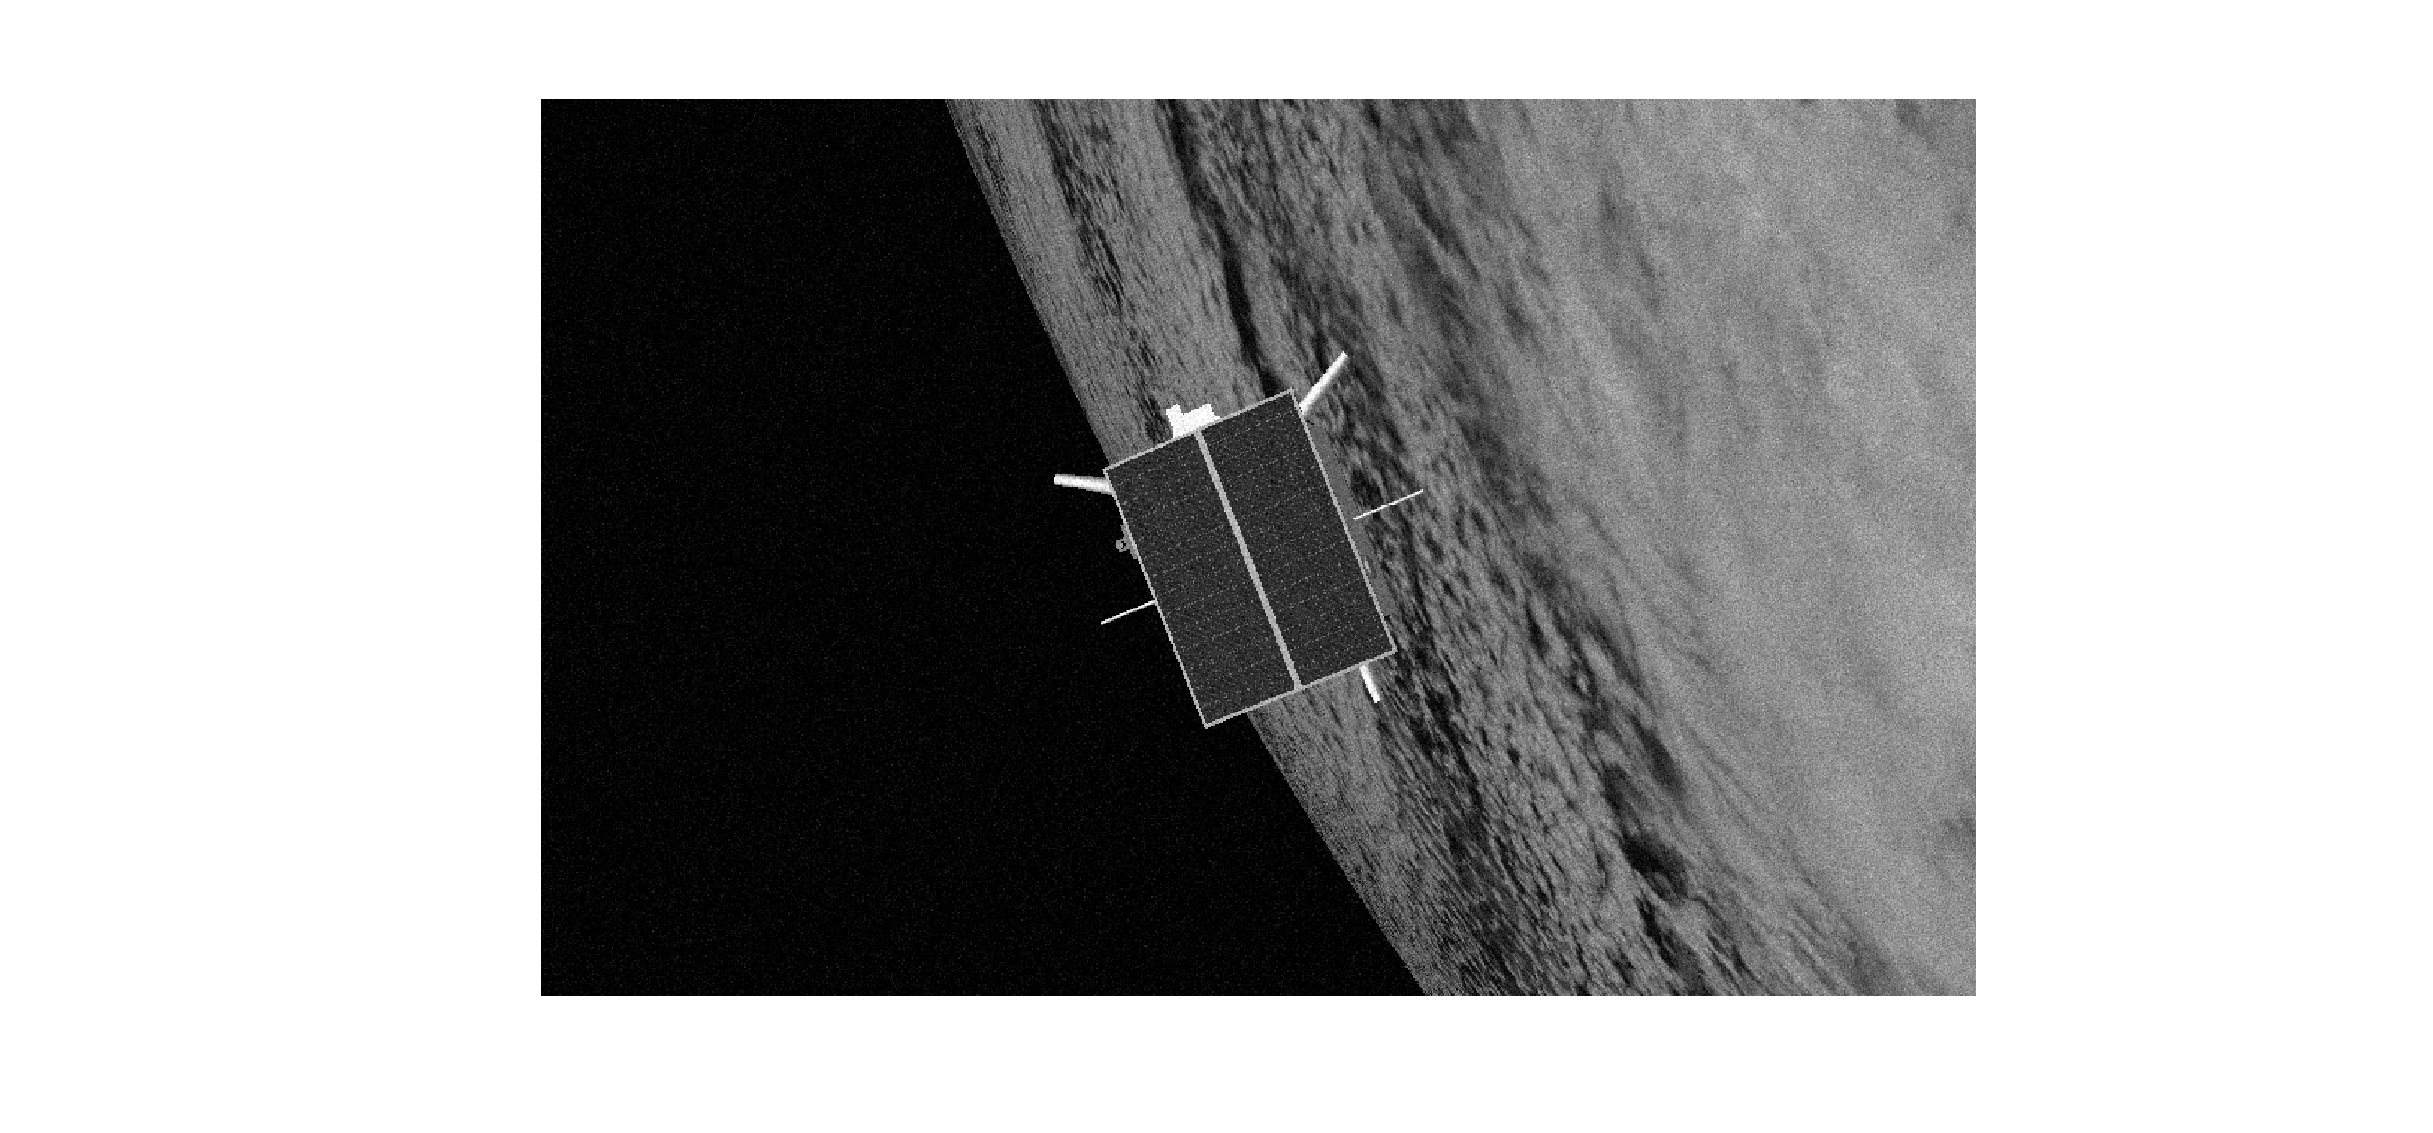
\includegraphics[width=0.4\textwidth]{gfx/FeatureDetection/chosenImage.eps}}
  \qquad
  \subfloat[Gradient detection of original image]{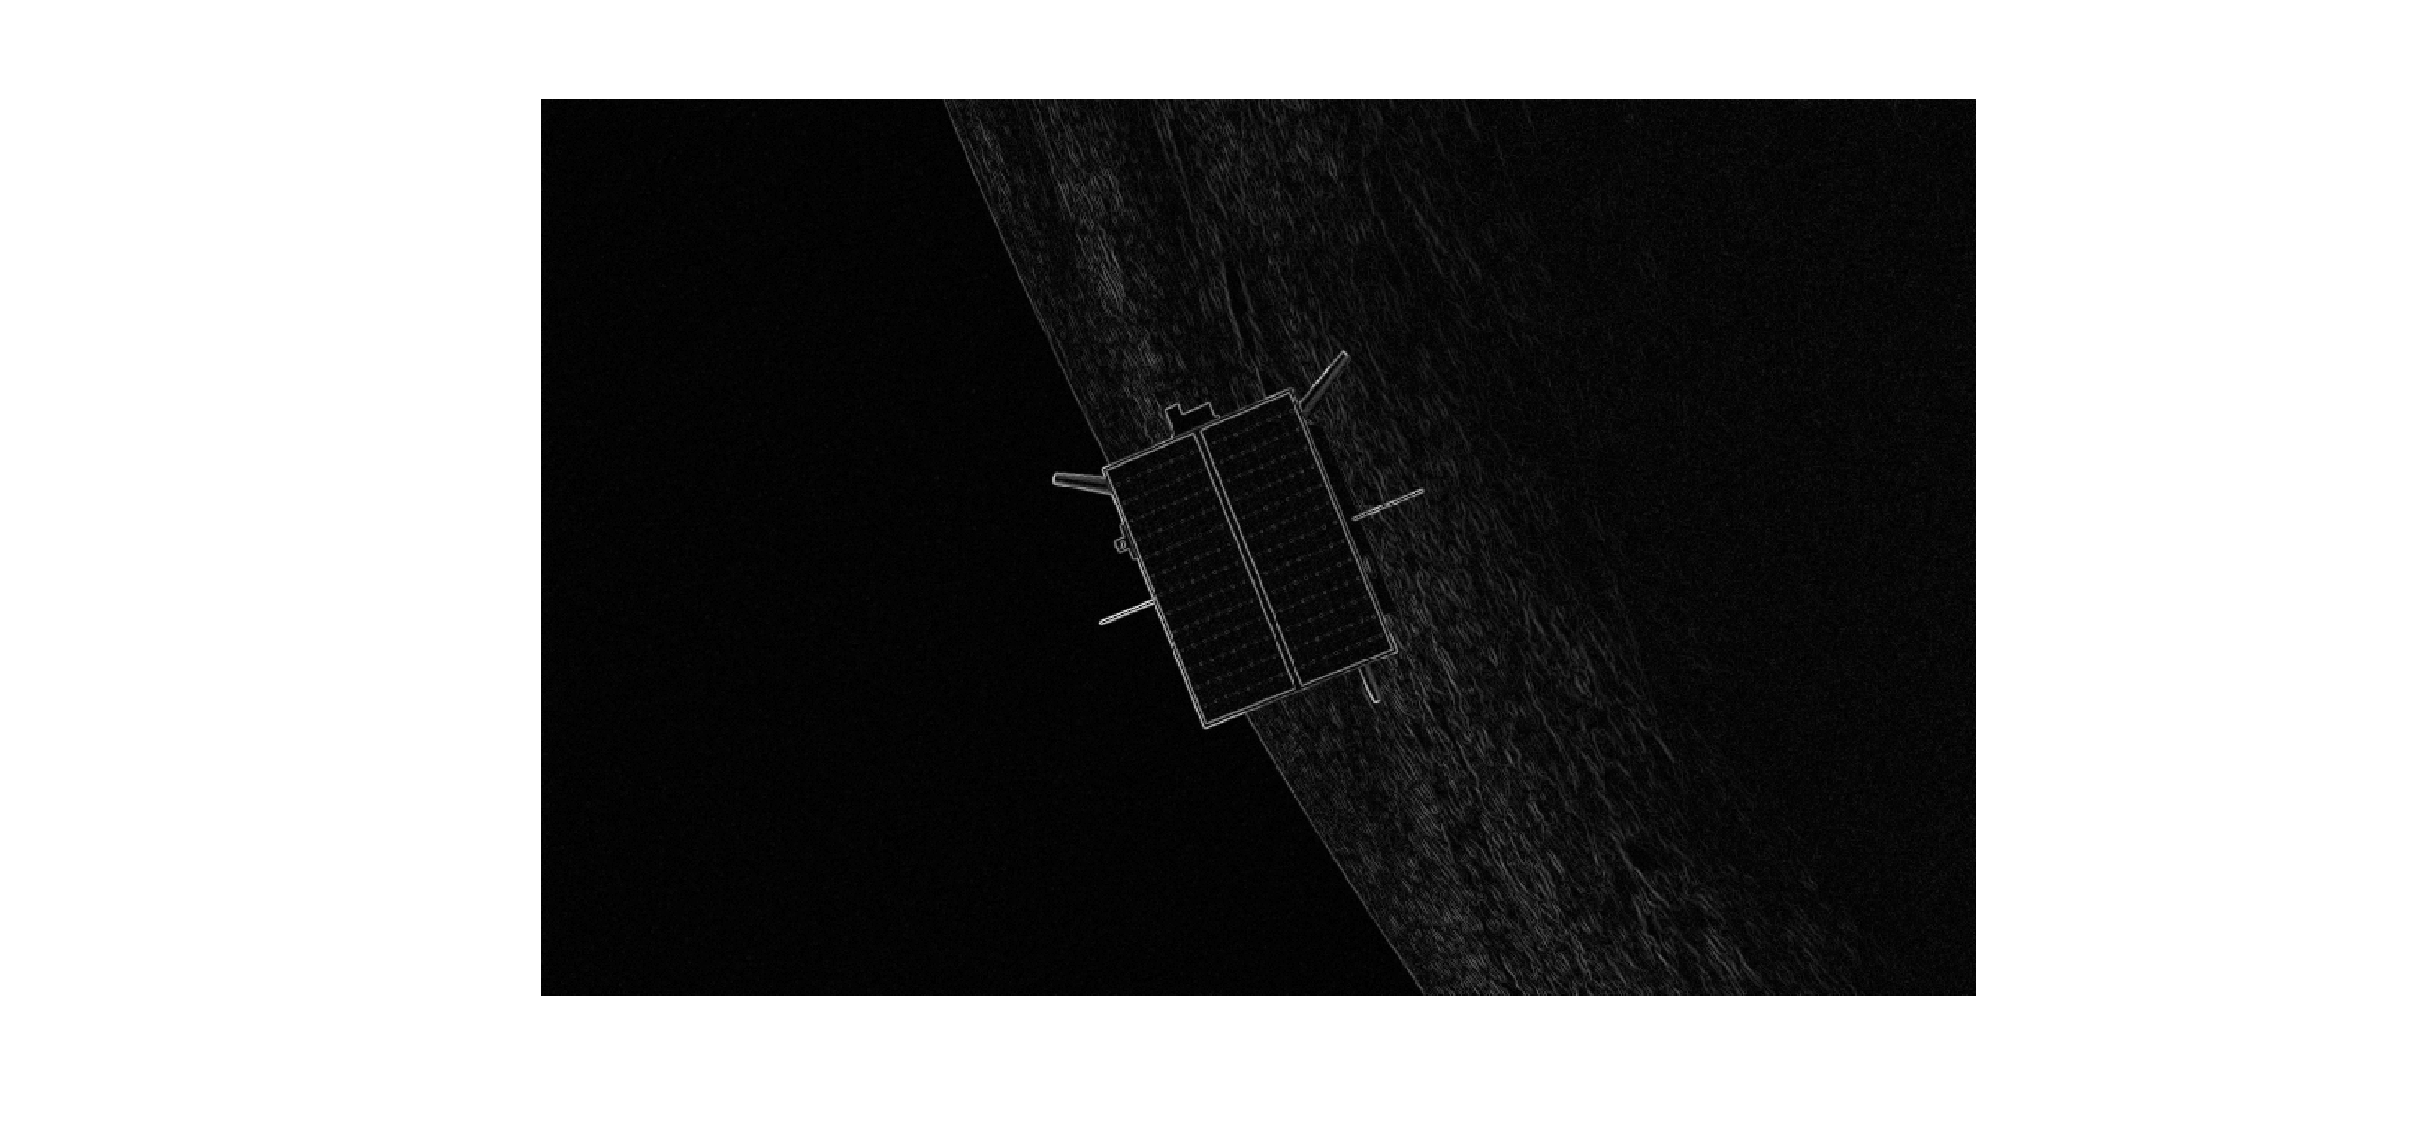
\includegraphics[width=0.4\textwidth]{gfx/FeatureDetection/gradientBeforeTresholding.eps}}
  \qquad
  \subfloat[Histogram of normalized gradient values]{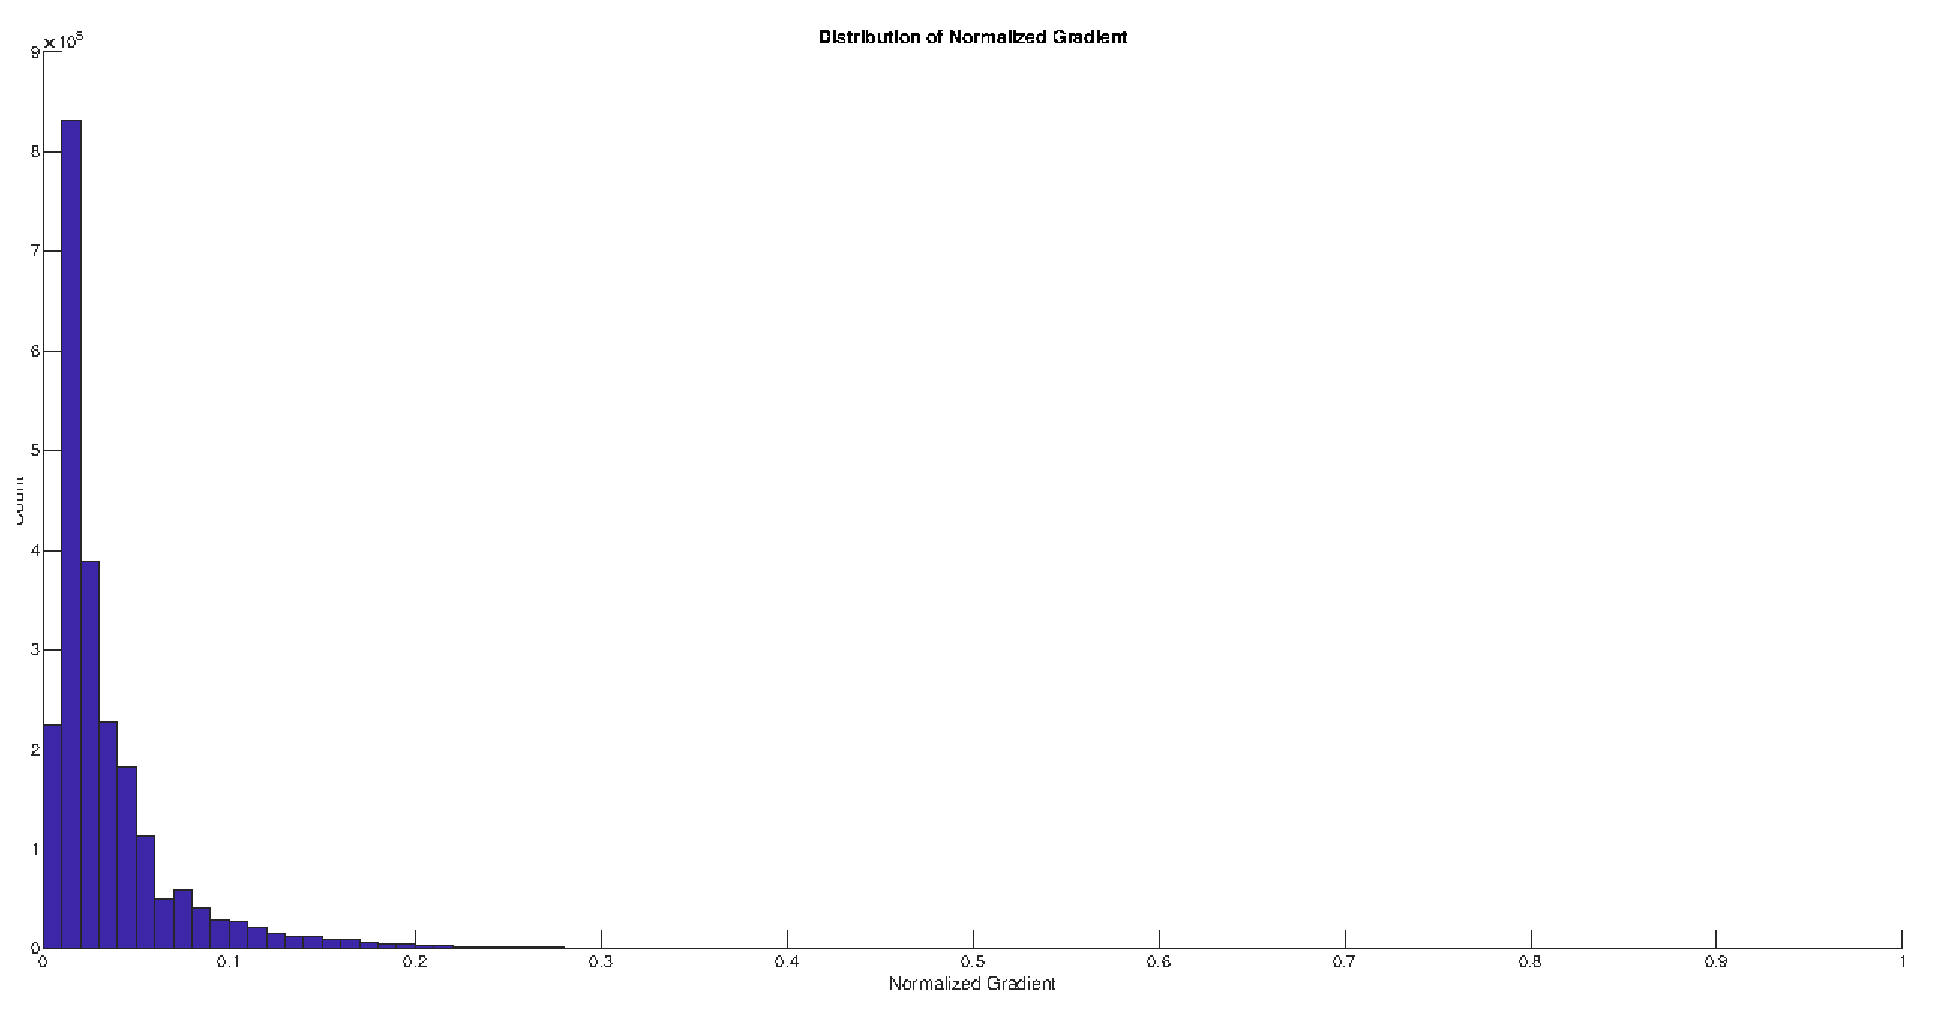
\includegraphics[width=0.4\textwidth]{gfx/FeatureDetection/gradientDistribution.eps}}
  \qquad
  \subfloat[Output filtered image gradients]{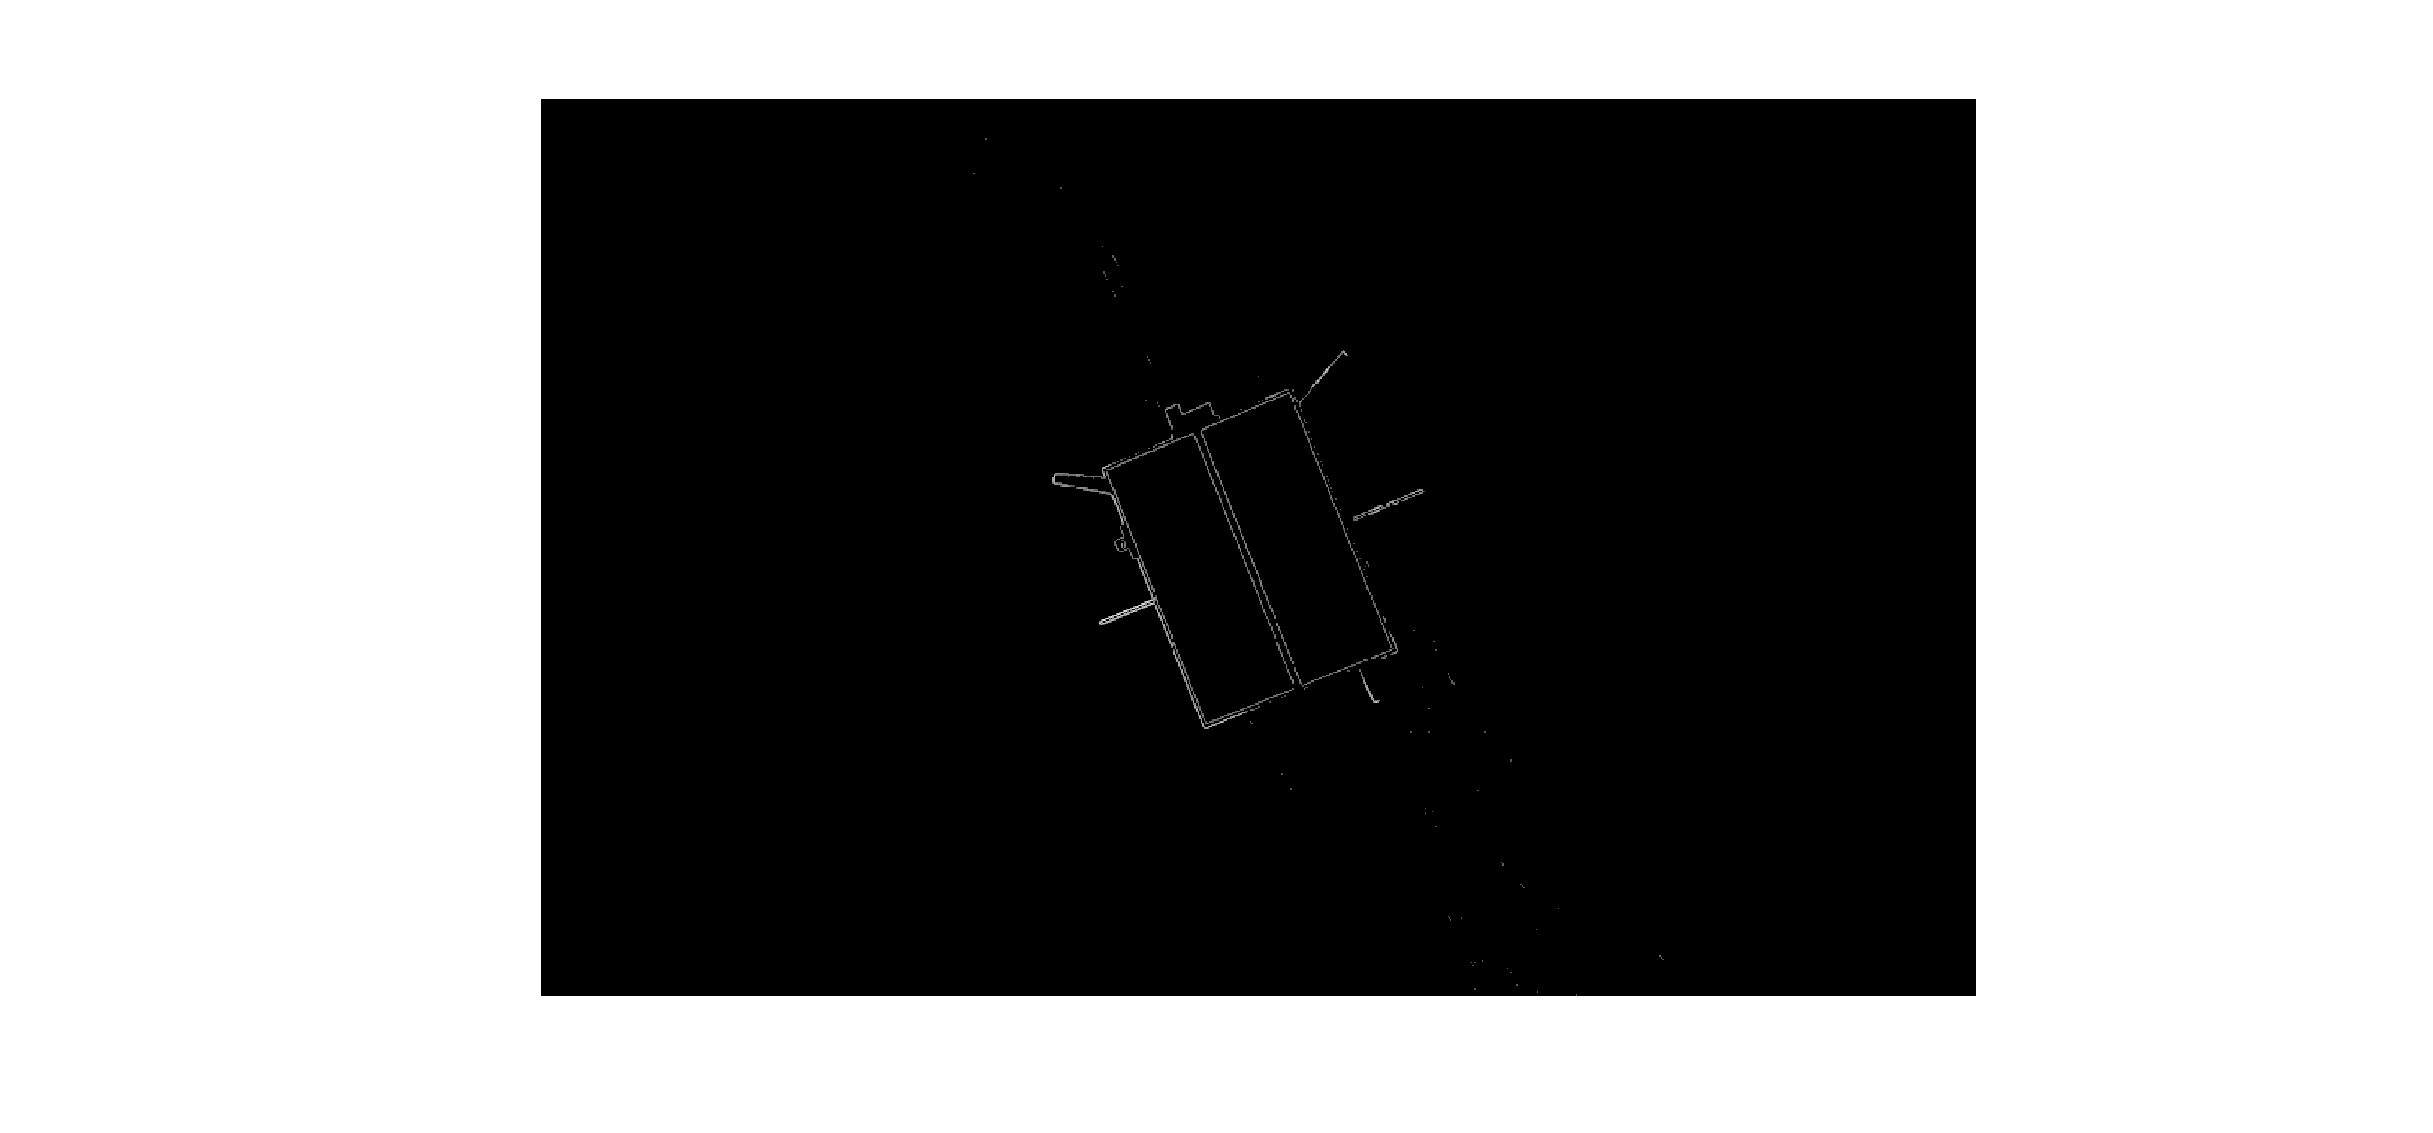
\includegraphics[width=0.4\textwidth]{gfx/FeatureDetection/imageAfterTresholding.eps}}
  \caption{Different steps of the \acrshort{wge}}
  \label{fig:wgeSteps}
\end{figure}

By computing the \acrfull{cdf} of the vertical and horizontal gradient of the filtered image obtained by the \acrshort{wge}, we can determine the coordinates of a \acrshort{roi} where the features that yield the strongest intensity variations are located. Then, assuming that the filtered image gradient is normally distributed, the \acrshort{roi} coordinates can be found by limiting each of the previously computed \acrshort{cdf}s between $0.025$ and $0.975$ in order to enclose the central $95\%$ of the normal distribution.

\begin{figure}[htbp]
  \centering
  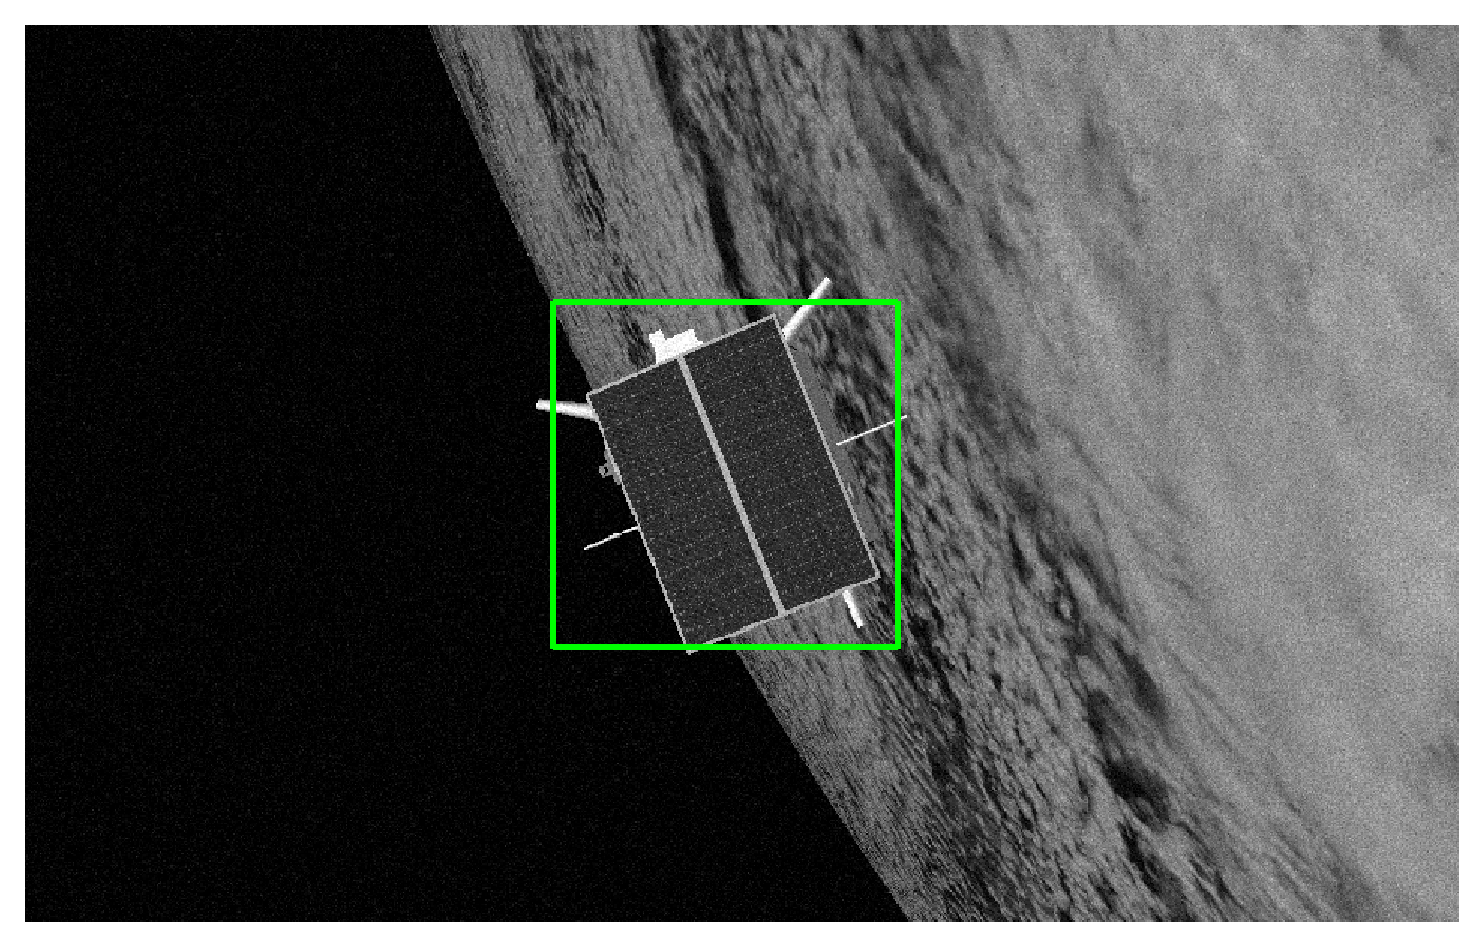
\includegraphics[width=0.82\textwidth]{gfx/FeatureDetection/ROI.eps}
  \caption{Result of the \acrshort{roi} detection procedure}
  \label{fig:ROI}
\end{figure}

As noted in \cite{fracchio2019}, for images having a composite background the \acrshort{roi} detection is limited by the presence of interference, so a smarter choice for selecting the bounding box limits is to treshold the \acrshort{cdf}s between $0.005$ and $0.95$. Therefore, only the central $90\%$ of the normal distribution is selected. Restricting the range however negatively affect the \acrshort{roi} detection procedure for images were the background is empty. This problem can be solved by taking into account an additional constant, equal to the $5\%$ of the mean edge length of the \acrshort{roi} for enlarging the \acrshort{roi} boundaries.

\begin{figure}[htbp]
  \centering
  \subfloat[\acrshort{roi} selected by considering only the central $90\%$ of the normal distribution]{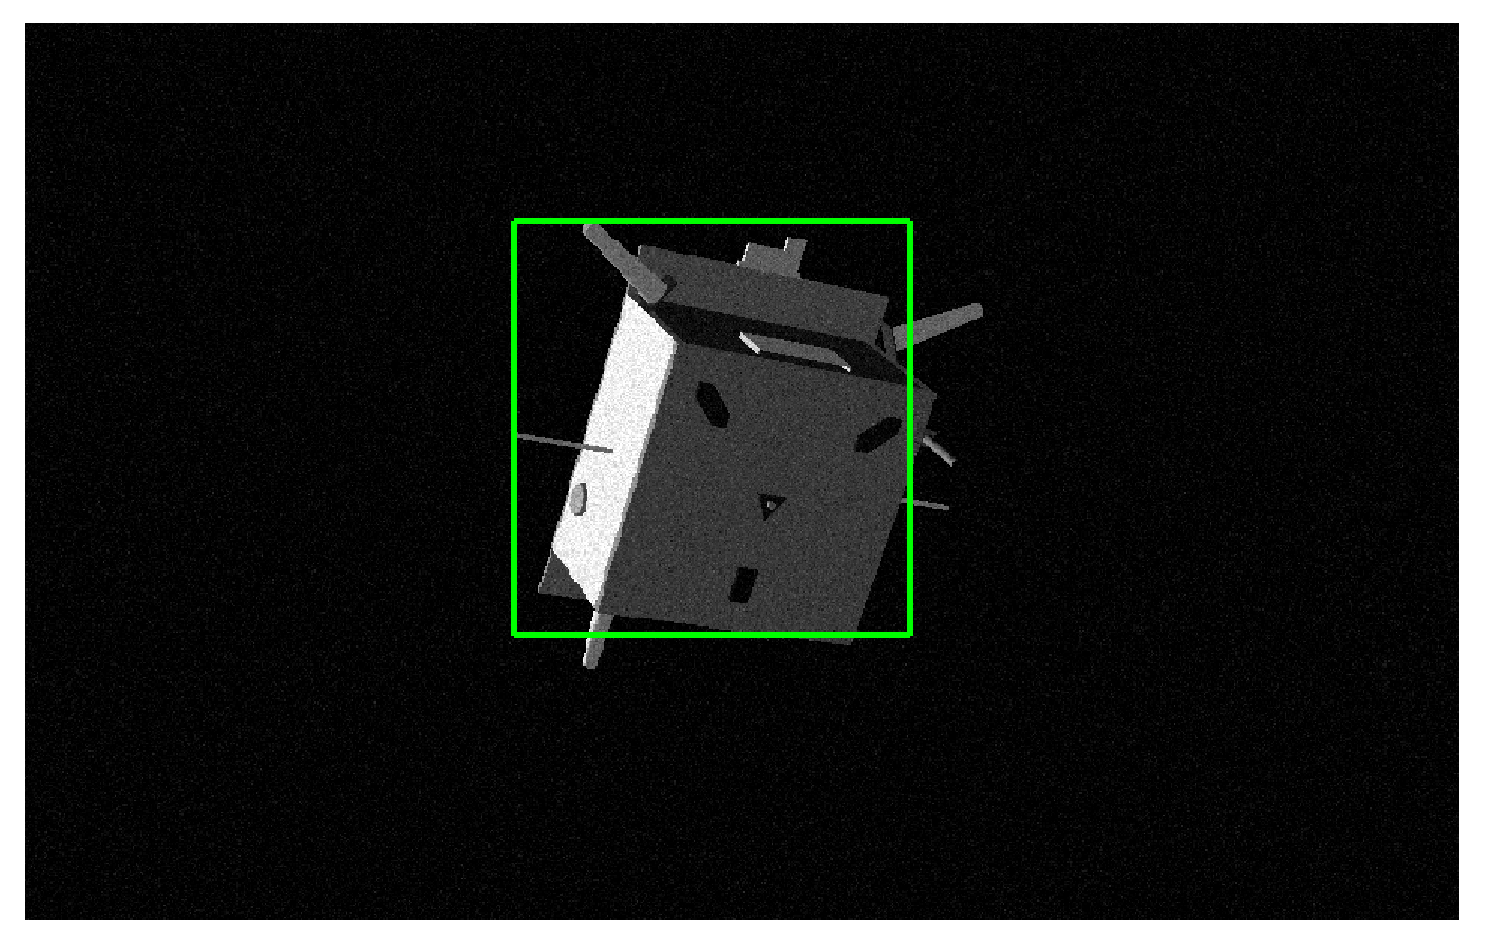
\includegraphics[width=0.45\textwidth]{gfx/FeatureDetection/ROInoConstant.eps}}
  \qquad
  \subfloat[\acrshort{roi} enlarged by adding the $5\%$ of the mean edge length of the previously \acrshort{roi}]{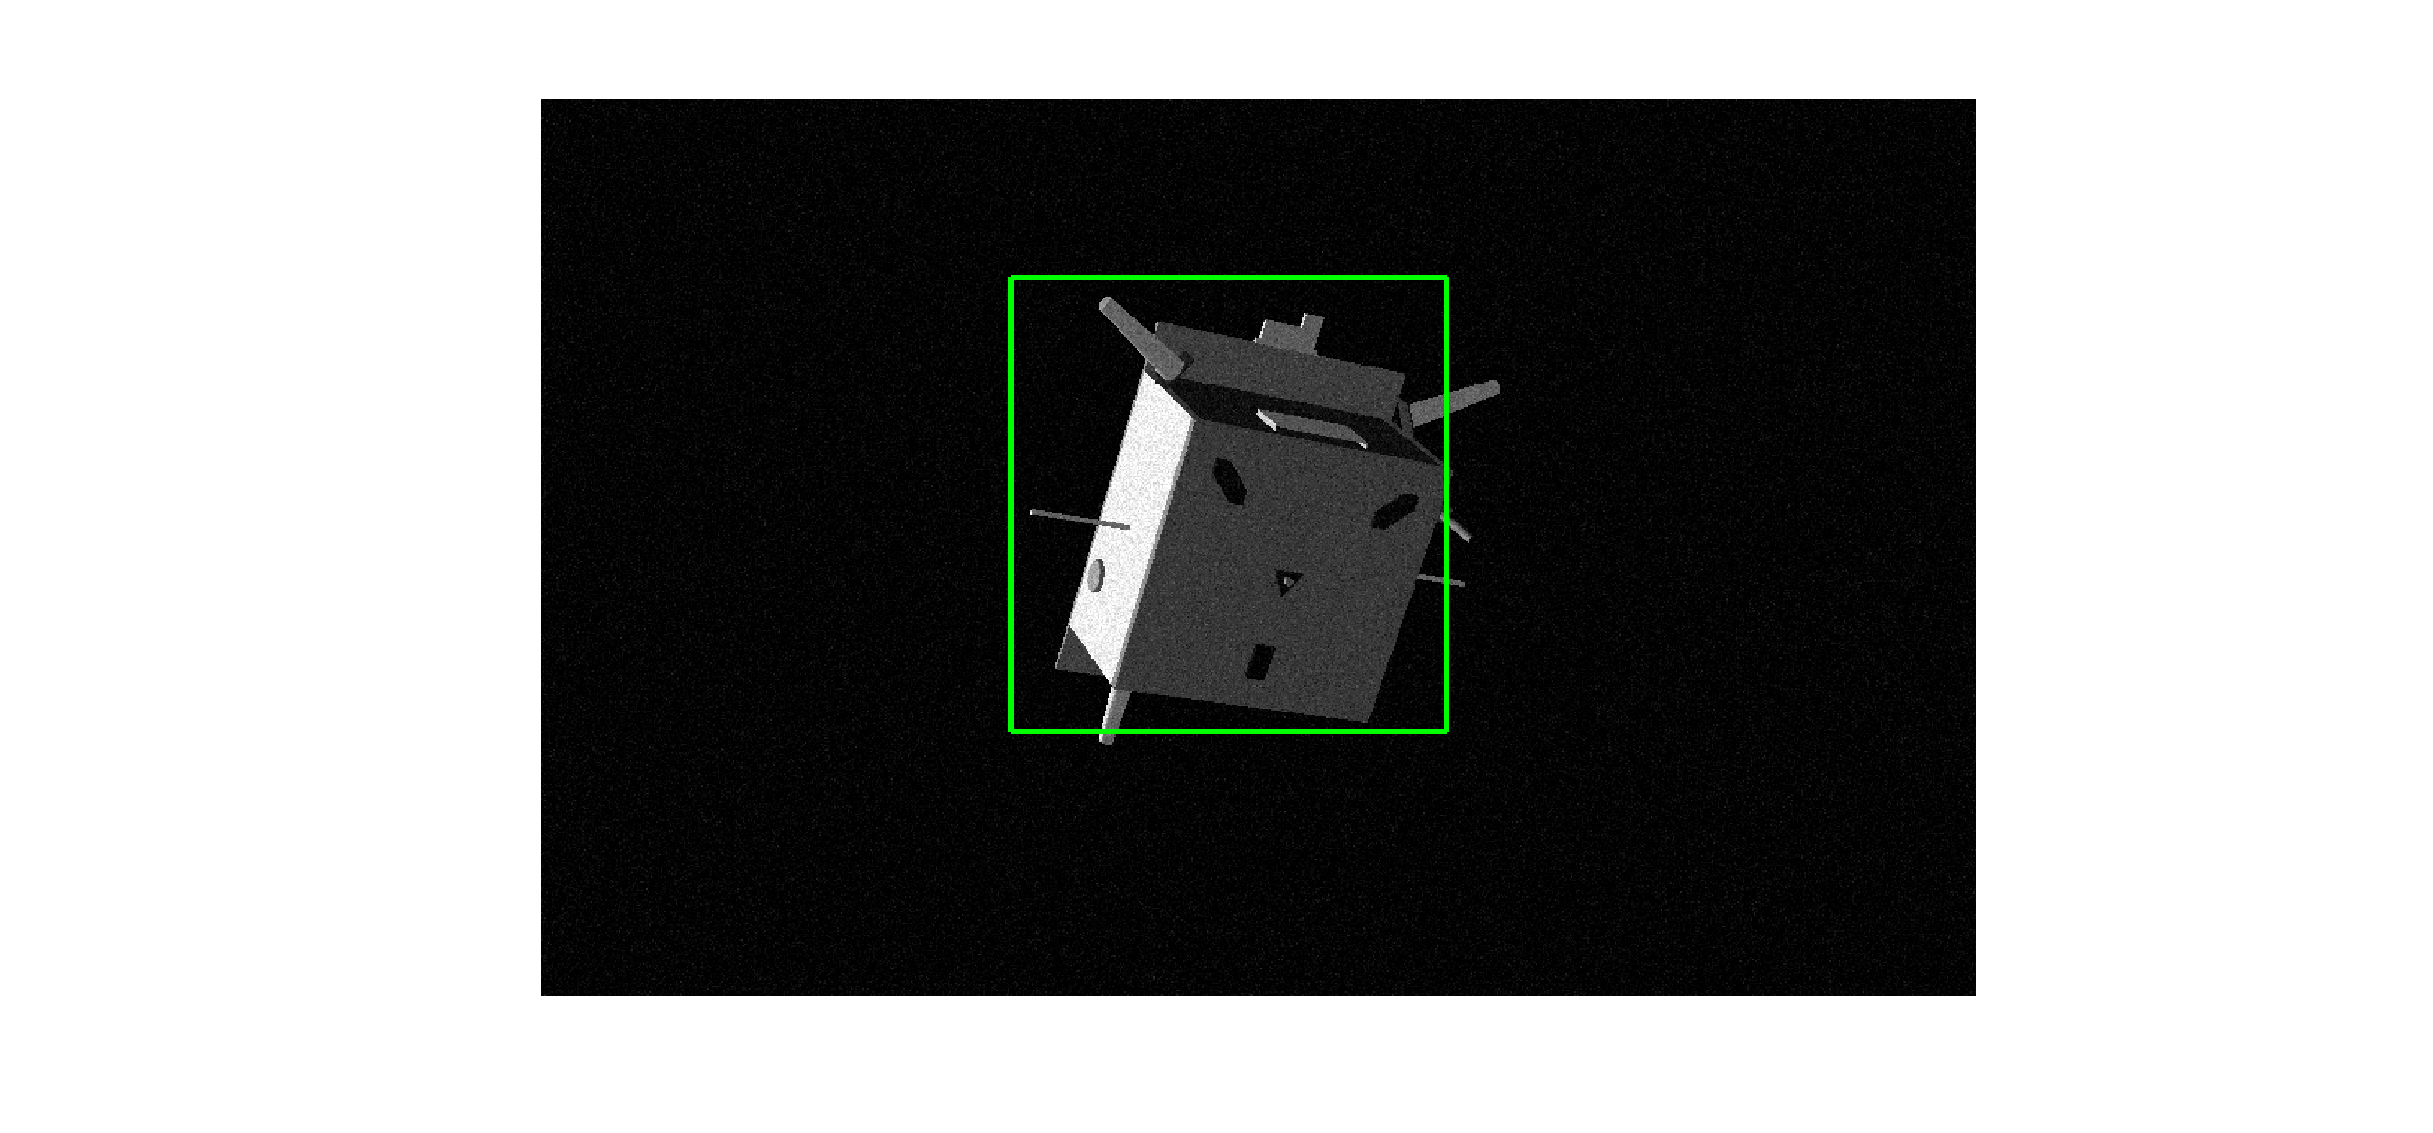
\includegraphics[width=0.45\textwidth]{gfx/FeatureDetection/enlargedROI.eps}}
  \caption{Improving the \acrshort{roi} detection procedure}
  \label{fig:roicomparisons}
\end{figure}

One of the innovative features of the \acrshort{wge} technique is that, once the \acrshort{roi} is correctly determined, it is possible to compute a coarse estimation of the the relative position and line of sight even before the pose determination subsystem. By defining the diagonal length of the \acrshort{roi}, $l_{ROI}$, as:

\begin{equation}
l_{ROI} = \sqrt{{ROI_{width}}^2 + {ROI_{height}}^2} \,,
\end{equation}

a coarse estimation of the range to the target \acrshort{sc} from the origin of the camera frame is given by :

\begin{equation}
\norm{t_C}_2 = \frac{\nicefrac{((f_x+f_y)}{2}) L_C}{l_{ROI}} \,,
\end{equation}

were \gls{lc} denotes the diagonal characteristic length of the \acrshort{sc} \acrshort{3d} model. By knowing the coordinates of the center of the image, $[C_x, C_y]$ and the coordinates of the \acrshort{roi} center, $[B_x, B_y]$, it is possible to compute the azimuth and elevation angles ($\alpha, \beta$) from the origin of the camera frame, $C$, to the origin of the body-fixed coordinate system, $B$ :

\begin{equation}
\alpha = \arctan{\frac{B_x - C_x}{f_x}} \,,
\end{equation}

\begin{equation}
\beta = \arctan{\frac{B_y - C_y}{f_y}} \,.
\end{equation}

Once ($\alpha, \beta$) are known, the coarse relative position solution is given by : 

\begin{equation}
  t_C
  =
  \begin{bmatrix}
    \cos(\alpha) & 0 & -\sin(\alpha) \\
    0 & 1 & 0 \\
    \sin(\alpha) & 0 & \cos(\alpha)
  \end{bmatrix}
  \begin{bmatrix}
    1 & 0 & 0 \\
    0 & \cos(\beta) & \sin(\beta) \\
    0 & -\sin(\beta) & \cos(\beta)
  \end{bmatrix}
  \begin{bmatrix}
    0 \\
    0 \\
   \norm{t_C}_2
  \end{bmatrix} \,.
\end{equation}

\begin{figure}[htbp]
  \centering
  \includegraphics[width=0.65\textwidth]{gfx/coarsePoseEstimation.eps}
  \caption{Calculation of a coarse relative position solution using the WGE
technique \cite{Sharma2018}}
  \label{fig:imageProcessingSubsystem}
\end{figure}

In order to extract the features from the input image, a first edge detection process is applied to the tresholded image by means of the Hough transform. As briefly introduced in section \ref{sec:hough}, when applied to the problem of detecting straight lines into an image, the Hough transform performs a shape identification through a voting procedure in the paramter space ($\rho$, $\theta$).
When computing the Hough transform with MATLAB some hyperparameters are required, which for instance are :

\begin{itemize}
\item the desired resolution of $\rho$ and $\theta$, 
\item the maximum number of peaks to identify in the Hough transform matrix,
\item the expected minimum length of the the line segment, \gls{l_min},
\item procedure : the expected minimum length of the the line segment, \gls{lambda} and the maximum gap between two points to be considered in the same line segment, \gls{lambda}.
\end{itemize}

The geometrical constraints imposed to the Hough transform are dictated by the choice of \gls{l_min} and \gls{lambda}. Fixing a value of (\gls{l_min}, \gls{lambda}) for all the images will result into the inability of the algorithm to adapt to different distances between the camera and the target \acrshort{sc}. In fact, as the camera moves closer and closer to the target \acrshort{sc}, the latter will fill larger and larger portions of the image, and the expected lengths of its edges in the image plane are expected to grow, so a recomputation of the geometrical hyperparameters would be needed. However, it is reasonable to hypothesize that the size of the detected \acrshort{roi} bounding box will grow too, so, in \cite{Sharma2018} is proposed to scale the geometrical hyperparameters by using the information about the \acrshort{roi} diagonal length :

\begin{equation*}
L_{min,Hough} = \kappa_1 l_{ROI} \ \ \ \  \lambda_{Hough} = \kappa_2 l_{ROI}  \,,
\end{equation*}

were $\kappa_1$ and $\kappa_2$ are two scalars which can be empirically estimated by performing several test simulations on ground. 

The idea proposed in \cite{Sharma2018} is to tune the values of $\kappa_1$ and $\kappa_2$ in order to only extract short line segments from the tresholded image.

A second stream of features is then obtained by directly appling the Sobel operator, which has been shown in section \ref{sec:imagegradient}, to the unfiltered, rectified image, using the MATLAB function \inlinecode{MATLAB}{edge}. The Sobel operator is applied by imposing an intensity treshold equal to $0.04$. As proposed in \cite{fracchio2019}, in order to eliminate the pixel chunks belonging to smaller reflective elements from the output of \inlinecode{MATLAB}{edge}, it is possible to filter the output by using the MATLAB function \inlinecode{MATLAB}{bwareaopen}. Once defined a minimum pixel number $P$, \inlinecode{MATLAB}{bwareaopen} removes all connected components (objects) that have fewer than $P$ pixels from the input binary image. In contrast with what done in \cite{fracchio2019}, which sets $P = 10$ for all images, in this work the $P$ value is computed adaptively for each image exploiting the information about the \acrshort{roi} diagonal length :

\begin{equation*}
P = \lfloor \eta \ l_{ROI}
\end{equation*}

where $\lfloor$ is the commonly used symbol for the \inlinecode{MATLAB}{ceil} operator and $\eta$ is a multiplicative constants which can be tuned empirically.
After that, the Hough transform is applied again on the output produced by the Sobel operator in order to extract line segments corresponding to the silhouette of the large components of the target \acrshort{sc}. The knowledge the \acrshort{roi} location, obtained through the \acrshort{wge} technique, is now exploited to automatically reject any line segment for which the midpoint lies outside the \acrshort{roi} itself. Also for computing the \acrfull{seh} stream of features, in \cite{Sharma2018} is advised to scale the geometrical hyperparameters needed to compute the Hough lines by using the information about the \acrshort{roi} diagonal length :

\begin{equation*}
L_{min,Hough} = \kappa_3 l_{ROI} \ \ \ \  \lambda_{Hough} = \kappa_4 l_{ROI}  \,,
\end{equation*}

where again, $\kappa_3$ and $\kappa_4$  are two multiplicative constants which can be fixed in an offline phase before the mission.

\subsubsection{Merging Edges}
The output of the Hough transform often results in multiple truncated edges, especially when applied to the image processed by the \acrshort{wge}. Since fragmentation can increase uncertainty and increase the computational cost of feature matching and pose solving \cite{fracchio2019}, a section of the \acrshort{svd} architecture is dedicated to find and merge line segments which may corresponds to the same true line segment into a single line segment.
To check whether two line segments can be considered similar and merged into one single edge, it is possible to define some geometrical checks on the basis of the parameters $\rho$ and $\theta$, which are defined for each Hough line found using the MATLAB function \inlinecode{MATLAB}{hough}.
Considering the two line segments represented in \ref{fig:mergeEdges}a\footnote{Note that the segments are represented in the image coordinate system, were the positive x axis points to the right, the positive y axis points downward and the positive z axis points toward the direction given by $  \mathbf{\hat{z}} = \frac{\mathbf{\hat{x}} \wedge \mathbf{\hat{y}}}{\norm{\mathbf{\hat{x}} \wedge \mathbf{\hat{y}}}}$.}, it is possible to write their polar representation in the Hough space as:

\begin{equation}
l_1 \rho_1 = x \cos (\theta_1) +  y \sin (\theta_1) \,,
\end{equation}

\begin{equation}
l_2 \rho_2 = x \cos (\theta_2) +  y \sin (\theta_2) \,.
\end{equation}

\begin{figure}[htbp]
  \centering
  \subfloat[Original edge]{\includegraphics[width=0.4\textwidth]{gfx/segmentsPreMerge.eps}}
  \qquad
  \subfloat[Output merged edge]{\includegraphics[width=0.4\textwidth]{gfx/segmentsAfterMerge.eps}}
  \qquad
  \caption{Merging two truncated edges \cite{Sharma2018}}
  \label{fig:mergeEdges}
\end{figure}

The conditions of similarity proposed by \cite{Sharma2018} are then:

\begin{equation}
|\theta_1 - \theta_2| \leqslant	\theta_{tresh} \,,
\end{equation}

\begin{equation}
|\rho_1 - \rho_2| \leqslant	\rho_{tresh} \,,
\end{equation}

where $\theta_{tresh}$ and $\rho_{tresh}$ are set to be equal to the resolution of $\theta$ and $\rho$ in the Hough space. In \cite{fracchio2019} is proposed to scale the value of $\rho_{tresh}$ using the information about the \acrshort{roi} diagonal length in order to improve the identification of the spacecraft true edge :

\begin{equation}
\rho_{tresh} = \nu d_{ROI} \,,
\end{equation}

where $\nu$ is a multiplicative constant which can be set to be equal to the resolution of $\theta$ in the Hough space. In this work, this second approach has been preferred. 
Furthermore, it is imposed that the Euclidean distance between the farthest pair of endpoints of the two line segments must be less than $d_{tresh}$ :

\begin{equation}
d_{p_{1b}-p_{21}} \leqslant d_{tresh} \,,
\end{equation}

where $d_{tresh}$ is computed for each image as half of the mean length of the detected segments :

\begin{equation}
d_{tresh} \leqslant {\frac{1}{2}} \overline{(l_1, l_2,\ldots, l_n)} \,.
\end{equation}

If the similarity conditions are met, then the two line segments are replaced with the line $l_3$, which is the line segment which joins the two farthest endpoints of $l_1$ and $l_2$ :

\begin{equation}
l_3 \rho_3 = x \cos (\theta_3) +  y \sin (\theta_3) \,.
\end{equation}

The Hough parameters which defines $l_3$ can be computed as follows\footnote{Note that the computation is done in the image coordinate system previously defined}. First, the angle between the positive x-axis and the joined segment is retrieved\footnote{Note that it is necessary to subtract $90^{\circ}$ from the computed angle to take into account that in the image coordinate system negative the quadrant is the upper while the positive one is the lower} :

\begin{equation}
\alpha_3 = 90^{\circ} - \arctan{\left(\frac{p_{1a,x}-p_{2b,x}}{p_{1a,y}-p_{2b,y}}\right)}
\end{equation}

from which it follows the value of $\theta_3$

\begin{equation}
\theta_3 = \alpha_3 - 90^{\circ}
\end{equation}

\begin{figure}[htbp]
  \centering
  \includegraphics[width=0.45\textwidth]{gfx/hough_rho_theta_diagram.eps}
  \caption{$\rho$ and $\theta$ diagram}
  \label{fig:theposeproblem}
\end{figure}

Now, to find $\rho_3$ it is sufficient to compute the intersection between a line which passes trough the origin and the joined segment :

\begin{equation}
m = \tan(\alpha_3)
\end{equation}

\begin{equation}
x = \frac{m_3(p_{1a,x}-p_{1a,y})}{\nicefrac{1}{m_3} + m_3} \,,
\end{equation}

\begin{equation}
y = - \frac{1}{m_3} x_3 \,,
\end{equation}

\begin{equation}
\rho_3 = x \cos (\theta_3) +  y \sin (\theta_3) \,.
\end{equation}

For what concerns the \acrshort{seh} stream instead, after the Hough transform is applied, the output image is fed to a function which removes all the lines which midpoints are located outside the \acrshort{roi}.

\subsubsection{Merge Streams}

\subsubsection{Feature Synthesis}

\subsubsection{Perceptual Grouping}

\subsection{Model Matching and Pose Determination}

\subsubsection{Feature Correspondence}

\subsubsection{Pose Determination}

\section{Conclusions}

% inserisci una tabella riassuntiva con tutti i parametri utilizzati
\cleardoublepage{}
\chapter{Results\label{chap:fourth-chapter}}
\begin{quotation}
{\footnotesize
\noindent{\emph{``Prediction is very difficult, especially if it's about the future.''\\}
}
\begin{flushright}
Niels Bohr
\end{flushright}
}
\end{quotation}
\vspace{0.5cm}

\section{Mathematical Preliminaries}

\subsection{Pinhole Camera Model}
%review of solution methods

\subsection{Image derivatives}
%review of solution methods

\subsection{The Hough Transform}
%review of solution methods

\subsection{Perspective-n-Point problem}
%review of solution methods

\section{Feature-based pose estimation implementation}

\subsection{Architecture}

\subsection{Image processing subsystem}

\subsubsection{Feature Detection}

\subsubsection{Feature Synthesis}

\subsection{Pose Determination}

\subsubsection{Feature Correspondence}

\subsubsection{Pose Refinement}



\cleardoublepage{}

%%%%%%%%%%%%%%%%%%%%%%%%%%%%%% Conclusion
\chapter*{Conclusions}
\addcontentsline{toc}{chapter}{Conclusions}
\markboth{Conclusions}{Conclusions}
%The conclusions must recall the field of work, the purpose of the thesis, what has been done and an evaluation of the obtained results.
%Furthermore, the conclusion must also emphasize the future prospects and must show how to move forward in the study area.
\begin{quotation}
  {\footnotesize
    \noindent{\emph{``If you didn't get angry and mad and frustrated, that means you don't care about the end result, and are doing something wrong.''\\}
    }
    \begin{flushright}
      Greg Kroah-Hartman
    \end{flushright}
  }
\end{quotation}
\vspace{0.5cm}

This project was successful in developing a tool which allows the end user to produce hundreds of images of a target \acrshort{sc} given its \acrshort{stl} model, using the open source ray tracer \acrshort{povray} in conjunction with MATLAB. The full uncontrolled dynamics of the target \acrshort{sc} has been simulated as well, so, if the inertial properties of the target are known, is possible to closely simulate the dynamical behavior of the target itself and from that, generate the images. Optionally is possible to also insert the Earth in the background, which enhances the realism of the scene. In particular, a great care has been putted into taking in consideration both the optical properties of the Earth surface and of the \acrshort{sc} surface.
The generated data-set has been then compared to the freely available SPEED data-set both in terms of a qualitative assessment (by comparing the histograms) and by applying a \acrshort{cv} algorithm.
The preliminary results obtained from the comparison shows that similar results have been obtained.
Still, there is room for improvement. Such as enhancing the model of the Earth to make it comparable with what found on the SPEED data-set. For what concerns the model of the \acrshort{sc} instead, more realistic texture could be used, if available. A better modeled surface would result in more accurate images produced and a better study could be made to better model the optical properties of the materials which covers the \acrshort{sc}. Moreover, overall rendering times when the Earth is in background are really long, as Earth rendering is a high demanding application. A possible improvement could be to find a way to cut the texture and Earth using not the full sphere but a subset with a mesh, for example. Or better, to patch the ray tracer source code to allow performing the rendering step on the GPU.
Concerning the image analysis instead, different pose solvers could be tried. In this work, a MATLAB builtin function has been used. Different pose solver could be used, such as the \textit{e}\acrshort{pnp} \cite{10.1007/s11263-008-0152-6} to make a comparison in terms of efficiency. Another improvement could be to employ separated Hough transforms to detect different geometric shapes, as suggested also in \cite{Sharma2018}. In general, the image processing subsystem still has to be improved, as it is susceptible to producing spurious edges, especially when the target is far distant from the camera or when the solar panel are not in shadow (so, when they are hitted directly from the Sun's light).
Imagining to implement the algorithm on an embedded board, the proposed toolbox also allows the set-up of hardware in the loop experiments to evaluate the computational time on real H/W.
Moreover, having available a toolbox capable of producing hundreds of images at will, also enables to implement completely different strategies for pose determination, such as the one based on neural networks like for example what proposed in \cite{Sharma2019} and compare the results with what obtained implementing more traditional techniques such as the ones used in this project.
\cleardoublepage{}

%%%%%%%%%%%%%%%%%%%%%%%%%%%%%% Bibliography
\bibliographystyle{plain}
\bibliography{bibliography}
\cleardoublepage{}

%%%%%%%%%%%%%%%%%%%%%%%%%%%%%% Appendices
\appendix
%%% Appendix A
\chapter{First appendix: Attitude and Orbit Simulator \label{app:first-appendix}}
In this appendix the kinematic and dynamic representation used for the simulation of the attitude of the target spacefrat will briefly be descripted.

\section{Keplerian Motion}
The dynamics of the \acrshort{cg} of a rigid body is given by Newton equation of motion stating that the variation in time of the linear mentum is equal to the external forces applied to the body, with respect to an inertial reference frame. Thus :

\begin{equation}
  \frac{d}{dt} (\textit{m} \mathbf{v}) = \sum\limits_{i=1}^n \mathbf{f_i}
\end{equation}

where $\textit{m}$ is the mass of the body, $\mathbf{v}$ its velocity and $\mathbf{f_i}$ the forces applied to the system. Then, for a rigid body orbiting around a single massive body, the main force to take into account is the gravitational pull that can be modelled accordingly to Newton law of gravitation as follows :

\begin{equation}
  \label{eqn:orbiteqtn}
  m \mathbf{\ddot{r}} = - \frac{\mu \textit{m}} {\norm{\mathbf{r}}^3} \mathbf{r} + \mathbf{f}
\end{equation}

where $\mu$ is the gravitational constant of the main attractor, $\mathbf{r}$ the position vector of the orbiting body computed from the main attractor \acrshort{cg} and $\mathbf{f}$ the sum of other forces applied to the system. The underlying assumption is to consider the main attractor to be still or moving in linear constant motion, which is never the case. Such assumptions holds well enough for many problem of interest. Considering null or negligible other forces it follows that the system motion is central, thus the angular momentum is conserved.\\
Such quantity, for this system, is defined as follows

\begin{equation}
  \mathbf{h} = \mathbf{r} \wedge \mathbf{r}
\end{equation}

where $\mathbf{v}$ is the velocity, derivative of the position vector $\mathbf{r}$ expressed in the said reference frame.\\
Crossing \ref{eqn:orbiteqtn} with the angular momentum and considering that the gravitational field is conservative, it is possible to determine the position of the orbiting body in time through six parameters that represent the analytical solution of the restricted two body problem. For this research the influence of other massive bodies is not taken into account as for many of the applications here considered can be analysed considering satellites to be small bodies close to the planet.\\
The most used set of parameters are often referred to as Keplerian parameters, however different parametrization are possible. Of these six constant two represent the shape of the orbit, which must be a conic according to Kepler's studies and Newton's formulation, three identify the orientation of the orbit in a \acrshort{3d} space and the last one links the position along the orbital with time. The shape is identified by the semi-major axis a of the conic and the eccentricity e, restricted to be between zero and one for closed orbits, being zero for circular orbits. In the reference frame with z axis aligned with angular momentum and x axis aligned with the minimum orbital distance (eccentricity vector) the position vector can be written as follows

\begin{equation}
  \mathbf{r_{orb}} = \frac{\nicefrac{\norm{h}^2}{\mu}}{1 + e cos \theta} \begin{Bmatrix} cos \theta
    \\ sin \theta
    \\ 0
  \end{Bmatrix} = \frac{a(1-e^2)}{1+ e cos \theta} \begin{Bmatrix} cos \theta
    \\ sin \theta
    \\ 0
  \end{Bmatrix}
\end{equation}

Then the position vector $\mathbf{r_{orb}}$ in this frame can be translated back into the inertial $\mathbf{r}$ by using three sequential rotations in the order \textit{z} - \textit{x} - \textit{z} according to the values of the other three parameters: argument of pericenter $\omega$ , inclination \textit{i} and right ascension of the ascending node $\Omega$.


\section{Dynamics}

\subsection{Euler Equations}

The dynamics of a rigid body which is tumbling into space can be modeled by mean of the well known Euler equations, having in mind that such equation is expressed in a non-inertial reference frame attached to the body frame :

\begin{equation}
  \dot{\mathbf{\omega_T}} = \mathbf{(I_T)}^{-1} \left[\mathbf{L_T} - \mathbf{\omega_T}  \wedge (\mathbf{I_T} \mathbf{\omega_T})\right]
\end{equation}

where \textbf{$\omega_T$} is the angular velocity vector of the spacecraft in body frame, \textbf{$I_T$} is the inertia tensor of the spacecraft in body frame and \textbf{$L_T$} are the external torques acting on the spacecraft due to  external disturbances and control torques.

\section{Direct Cosine Matrix}
The direct cosine matrix, or attitude matrix, gives the transformation of a vector from a reference frame $N$ to another reference frame $O$ :

\begin{equation}
  \mathbf{r_{O}} = \mathbf{A_{ON}} \mathbf{r_{N}}
\end{equation}

So, if we consider the spacecraft body frame and the inertial frame, then we can write the relation between the two frames as :

\begin{equation}
  \mathbf{r_{T}} = \mathbf{A_{TN}} \mathbf{r_{N}}
\end{equation}

As it is demonstrated in Ref. \cite{Markley2014}, we can express the time dependence of the attitude matrix by writing the rotation from the body frame to the inertial frame as :

\begin{equation}
  \dot{A}_{TN}= - [\omega_{TN} \times]A_{TN}
\end{equation}

where $[\omega_{TN} \times]$ is the skew-symmetric cross product matrix containing the components of the angular velocity vector :

\begin{equation*}
  \mathbf{[\omega \times]} =
  \begin{bmatrix}
    0                & -\omega_{TN_{3}} & \omega_{TN_{2}}  \\
    \omega_{TN_{3}}  & 0                & -\omega_{TN_{1}} \\
    -\omega_{TN_{2}} & \omega_{TN_{1}}  & 0
  \end{bmatrix}
\end{equation*}

Thus, by integrating this relation, we can get full attitude at every iteration.

\subsection{Environmental Disturbances} \label{sec:disturbances}
The external disturbances acting on spacecraft placed in a LEO orbit are basically four and are due to :

\begin{itemize}
  \item Gravity Gradient
  \item Magnetic Field
  \item Solar Radiation Pressure
  \item Aerodynamic Drag
\end{itemize}

Details about how those torques have been mathematically modeled will be given in the following sections.

\subsubsection{Gravity Gradient}
Any non-symmetrical rigid body in a gravity field is subject to a gravity-gradient torque.
If we consider a rigid spacecraft, the torque due to the gravity gradient about the spacecraft's center of mass can be modeled as :

\begin{equation}
  \mathbf{L_{gg}} = \frac{3 \ mu}{r^3} \mathbf{n} \wedge (\mathbf{I} \ \mathbf{n})
\end{equation}

where $\mu$ is the Eart's gravitational constant, $\textbf{r}$ is the radius vector from the center of the Earth, thus $r \equiv \Vert{\textbf{r}}\Vert$, $\textbf{I}$ is the inertia tensor in body frame and $\textbf{n}$ is the body frame representation of a nadir-pointing unit vector.\\
Further details about the model can be found in reference \cite{Markley2014}.

\subsubsection{Earth's Magnetic Field}
The torque generated by a magnetic dipole $\textbf{m}$ in a magnetic field $\textbf{B}$ is

\begin{equation}
  \mathbf{L_{mag}} = \mathbf{m} \wedge \mathbf{B}
  \label{eq:magfield}
\end{equation}

where $\mathbf{B}$ is the magnetic field in the body frame.
The most basic source of a magnetic dipole is a current loop. A current of I amperes flowing in a planar loop of area A produces a dipole moment of magnitude m=IA in the direction normal to the plane of the loop and satisfying a right-hand rule.
When $\textbf{m}$ is in $Am^2$ and the magnetic field is specified in Tesla, Eq. \ref{eq:magfield} gives the torque in $Nm$. If there are N turns of wire in the loop, the dipole moment has magnitude m=NIA (such as the case of a magnetic torquer).
To model $\textbf{B}$ either the full IGRF model or the simple dipole model can be used.\\
For what concerns this work, the full IGRF model truncated to the 10th order has been used. Further details about the model can be found in reference \cite{Davis2014}

\subsubsection{Solar Radiation Pressure}
Solar radiation pressure acting on the surfaces of the spacecraft causes a disturbance torque that in general, cannot be neglected for orbits higher than \SI{800}{\kilo\meter}, so it has been taken into account in this work.
The SRP torque is zero zero when the spacecraft is in the shadow of the Earth or any other body, of course.
To take into account the effect of solar radiation pressure on the spacecraft, the spacecraft's surface can be modeled as a collection of $N$ flat plates of area $S_{i}$, outward normal $\mathbf{n_{b}}$ in the body coordinate frame, specular reflection coefficient $\rho_s$, diffuse reflection coefficient $\rho_{d}$ and absorption coefficient $\rho_{a}$; those coefficients must sum to unity.
For what concerns this work, only $\rho_s$ and $\rho_d$ have been considered, since all the absorbed radiation is emitted as thermal radiation,  although not necessarily at the same time or from the same surface as its absorption.
For an accurate modeling of thermal radiation we must also known the absolute temerature and the emissivity of each surface.
We can define the spacecraft-to-Sun unit vector in the spacecraft's body frame as :

\begin{equation}
  \mathbf{s_t} = \mathbf{A_{TN}} \mathbf{s_i}
\end{equation}

where $\mathbf{A_{TN}}$ is the attitude matrix and $\mathbf{s_i}$ is the spacecraft-to-Sun unit vector in the GCI frame.
We can define the angle between the Sun vector and the normal exiting from the normal to the i-th plate as :

\begin{equation}
  cos(\theta_{SRP}^{i}) = \mathbf{n}_{T}^{i} \cdot \mathbf{s_b}
\end{equation}

The SRP force on the i-th plate can be expressed as :

\begin{equation}
  \mathbf{F}_{SRP} = - P_{Sun}A_{i}\left[ 2\left( \frac{\rho_{d}^{i}}{3} + \rho_{s}^{i}cos(\theta_{SRP}^{i}) \right) \mathbf{n}_{B}^{i} + (1 -\rho_{s}) \mathbf{s_t} \right] max(cos(\theta_{SRP}^{i}),0)
\end{equation}

where $P_{Sun}$ is the solar radiation pressure.
The Solar radiation pressure torque acting on the spacecraft is then given by :

\begin{equation}
  \mathbf{L}_{SRP}^{i} = \sum\limits_{i=1}^n  \mathbf{r}_{i} \times \mathbf{F}_{SRP}^{i}
\end{equation}

where $\mathbf{r}_{i}$ is the vector from the spacecraft center of mass to the centre of pressure of the SRP on the i-th face.
In this formulation we are not considering the albedo radiation coming from the Earth and from the Moon.
Further details on how the solar radiation pressure, the spacecraft-to-Sun unit vector and the eclipse condition have been modeled can be found in reference \cite{Markley2014}.

\subsubsection{Aerodynamic Drag}
Aerodynamic torque is generally computed by modeling the spacecraft as a collection of $N$ flat plates of area $A_i$ and outward normal unit vector $\mathbf{n_{B}}$ expressed in the spacecraft body-fixed coordinate system. The torque depends on the velocity of the spacecraft relative to the atmosphere, which is not simply the velocity of the spacecraft in the GCI frame, because the atmosphere is not stationary in that frame.
The most common assumption is that the atmosphere co-rotates with the Earth. The relative velocity in the GCI frame is then given by :

\begin{equation}
  \mathbf{v_{relI}} =  \mathbf{v_I} + [\mathbf{\omega_{\earth} \times}] \mathbf{r_I}
\end{equation}

where $\mathbf{r_I}$ and $\mathbf{v_I}$ are the position and velocity of the spacecraft expressed in the GCI frame.
The Earth's angular velocity vector is $\mathbf{\omega_{\earth}} = \omega_{\earth}[0 0 1]'$ with $\omega_{\earth}$ = \SI{0.000072921158553}{\radian/\second}.
The velocity in the body frame is the computed as :

\begin{equation}
  \mathbf{v_{relT}} = \mathbf{A_{TN}}   \begin{bmatrix} \dot{x} + \omega_{\earth} y \\ \dot{y} - \omega_{\earth} x \\ \dot{x} \end{bmatrix}
\end{equation}

The inclination of the \textit{i-th} plate with respect to the relative velocity is given by :

\begin{equation}
  cos(\theta_{aero}^{i}) = \frac{\mathbf{n}_{T}^{i} \cdot \mathbf{v}_{rel\ T}}{\norm{\mathbf{v}_{rel}}}
\end{equation}

The aerodynamic force on i-th plate in the flat plate model is

\begin{equation}
  \mathbf{F}_{aero}^{i} = - \frac{1}{2} \rho C_{D} \norm{\mathbf{v}_{rel}} \mathbf{v}_{rel_{} T}\ S_{i}\ max(cos(\theta_{aero}^{i}),0)
\end{equation}

where $\rho$ is the atmospheric density, and $C_D$ is the drag coefficient.
$\rho$ can be modeled by mean of the well known exponential decaying model for the atmospheric density :

\begin{equation}
  \rho = \rho_{0} e^{(-(h-h_{0})/H)}
\end{equation}

where $\rho_{0}$ and $h_{0}$ are reference density and height, respectively, $h$ is the height above the ellipsoid and $H$ is the scale height, which is the fractional change in density with eight.
The value of $\rho_{0}$, $h_{0}$  and $H$ changes with $h$.
The values used to perform the simulation are the one given in \cite{Markley2014}.
The actual torque due to the aerodynamic drag can be computed as :

\begin{equation}
  \mathbf{L}_{aero}^{i} = \sum\limits_{i=1}^n  \mathbf{r}_{i} \times \mathbf{F}_{aero}^{i}
\end{equation}

where $n$ is the number of faces and $\mathbf{r}_{i}$ is the vector from the spacecraft center of mass to the center of pressure on the $i$ th face.
\cleardoublepage{}
%%% Appendix B
\chapter{Second appendix: Random Rotation Matrix Generation \label{app:second-appendix}}
\section{Kinematics}
In this section the kinematics representation used for the simulation will briefly be descripted. Two approach has been taken : 
\begin{itemize}
 \item [-] The DCM representation
 \item [-] The quaternion representation
\end{itemize}

\subsection{Direct Cosine Matrix}
The direct cosine matrix, or attitude matrix, gives the transformation of a vector from a reference frame $N$ to another reference frame $O$ : 

\begin{equation}
 \mathbf{r_{O}} = \mathbf{A_{ON}} \mathbf{r_{N}}
\end{equation}

So, if we consider the spacecraft body frame and the inertial frame, then we can write the relation between the two frames as : 

\begin{equation}
 \mathbf{r_{B}} = \mathbf{A_{B/N}} \mathbf{r_{N}}
\end{equation}

As it is demonstrated in Ref. \cite{Markley2014}, we can express the time dependence of the attitude matrix by writing the rotation from the body frame to the inertial frame as : 

\begin{equation}
 \dot{A}_{B/N}= - [\omega_{B/N} \times]A_{B/N} 
\end{equation}

where $[\omega_{B/N} \times]$ is the skew-symmetric cross product matrix containing the components of the angular velocity vector : 

\begin{equation*}
 \mathbf{[\omega \times]} =
                                \begin{bmatrix}
                                    0 & -\omega_{B/N_{3}} & \omega_{B/N_{2}} \\
                                    \omega_{B/N_{3}} & 0 & -\omega_{B/N_{1}} \\
                                    -\omega_{B/N_{2}} & \omega_{B/N_{1}} & 0
                                \end{bmatrix}
\end{equation*}

Thus, by integrating this relation, we can get full attitude at every iteration.

\subsection{Quaternions}
Quaternions are another way to parametrize the attitude of a rigid body in space. They are commonly used for control purpose due to the fact that they don't have kinematics singularities.
A quaternion is a four-component vector with some additional operations defined on it. A quaternion $\mathbf{q}$ has a three-vector part $\mathbf{q_{1:3}}$ and a scalar part $q_{4}$ : 

\begin{equation*}
 \mathbf{q} =
                                \begin{bmatrix}
                                    q_{1}\\
                                    q_{2}\\
                                    q_{3}\\
                                    q_{4}\\
                                \end{bmatrix}
\end{equation*}

The kinematic equation for the quaternion can be written as :

\begin{equation}
 \label{eq:quaternion}
 \dot{q} = \frac{1}{2} \mathbf{\varXi(\mathbf{q})} \mathbf{\omega_{B/N}}
\end{equation}

where $\mathbf{\varXi(\mathbf{q})}$ is defined as 

\begin{equation*}
 \mathbf{\varXi(\mathbf{q})} =
                                \begin{bmatrix}
                                   q_4 & -q_3 & q_2\\
                                   q_3 & q_4 & -q_1\\
                                  -q_2 & q_1 & q_4\\
                                  -q_1 & -q_2 & -q_3\\
                                \end{bmatrix}
\end{equation*}

By integrating Eq. \ref{eq:quaternion} can get the full attitude at every iteration in terms of quaternion.

\section{Dynamics}
\subsection{Euler Equations}
The dynamics of a rigid body which is tumbling into space can be modeled by mean of the well known Euler equations : 

\begin{equation}
  \mathbf{\omega_B} = \mathbf{(I_B)}^{-1} [\mathbf{L_B} - \mathbf{\omega_b}  \wedge (\mathbf{I_B} \mathbf{\omega_b})
\end{equation}

where \textbf{$\omega_B$} is the angular velocity vector of the spacecraft in body frame, \textbf{$I_B$} is the inertia tensor of the spacecraft in body frame and \textbf{$L_B$} are the external torques acting on the spacecraft due to  external disturbances and control torques.

\subsection{Environmental Disturbances} \label{sec:disturbances}
The external disturbances acting on spacecraft placed in a LEO orbit are basically four and are due to :

\begin{itemize}
  \item[-] Gravity Gradient
  \item[-] Magnetic Field 
  \item[-] Solar Radiation Pressure
  \item[-] Aerodynamic Drag
\end{itemize}

Details about how those torques have been mathematically modeled will be given in the following sections.

\subsubsection{Gravity Gradient}
Any non-symmetrical rigid body in a gravity field is subject to a gravity-gradient torque.
If we consider a rigid spacecraft, the torque due to the gravity gradient about the spacecraft's center of mass can be modeled as :

\begin{equation}
 \mathbf{L_{gg}} = \frac{3 \ mu}{r^3} \mathbf{n} \wedge (\mathbf{I} \ \mathbf{n})
\end{equation}

where $\mu$ is the Eart's gravitational constant, $\textbf{r}$ is the radius vector from the center of the Earth, thus $r \equiv \Vert{\textbf{r}}\Vert$, $\textbf{I}$ is the inertia tensor in body frame and $\textbf{n}$ is the body frame representation of a nadir-pointing unit vector.\\
Further details about the model can be found in reference \cite{Markley2014}.

\subsubsection{Earth's Magnetic Field}
The torque generated by a magnetic dipole $\textbf{m}$ in a magnetic field $\textbf{B}$ is

\begin{equation}
 \mathbf{L_{mag}} = \mathbf{m} \wedge \mathbf{B}
 \label{eq:magfield}
\end{equation}

where $\mathbf{B}$ is the magnetic field in the body frame.
The most basic source of a magnetic dipole is a current loop. A current of I amperes flowing in a planar loop of area A produces a dipole moment of magnitude m=IA in the direction normal to the plane of the loop and satisfying a right-hand rule.
When $\textbf{m}$ is in $Am^2$ and the magnetic field is specified in Tesla, Eq. \ref{eq:magfield} gives the torque in $Nm$. If there are N turns of wire in the loop, the dipole moment has magnitude m=NIA (such as the case of a magnetic torquer).
To model $\textbf{B}$ either the full IGRF model or the simple dipole model can be used.\\
For what concerns this work, the full IGRF model truncated to the 10th order has been used. Further details about the model can be found in reference \cite{Davis2014}

\subsubsection{Solar Radiation Pressure}
Solar radiation pressure acting on the surfaces of the spacecraft causes a disturbance torque that in general, cannot be neglected for orbits higher than \SI{800}{\kilo\meter}, so it has been taken into account in this work.
The SRP torque is zero zero when the spacecraft is in the shadow of the Earth or any other body, of course.
To take into account the effect of solar radiation pressure on the spacecraft, the spacecraft's surface can be modeled as a collection of $N$ flat plates of area $S_{i}$, outward normal $\mathbf{n_{b}}$ in the body coordinate frame, specular reflection coefficient $\rho_s$, diffuse reflection coefficient $\rho_{d}$ and absorption coefficient $\rho_{a}$; those coefficients must sum to unity.
For what concerns this work, only $\rho_s$ and $\rho_d$ have been considered, since all the absorbed radiation is emitted as thermal radiation,  although not necessarily at the same time or from the same surface as its absorption.
For an accurate modeling of thermal radiation we must also known the absolute temerature and the emissivity of each surface.
We can define the spacecraft-to-Sun unit vector in the spacecraft's body frame as : 

\begin{equation}
 \mathbf{s_b} = \mathbf{A_{B/N}} \mathbf{s_i}
\end{equation}

where $\mathbf{A_{B/N}}$ is the attitude matrix and $\mathbf{s_i}$ is the spacecraft-to-Sun unit vector in the GCI frame.
We can define the angle between the Sun vector and the normal exiting from the normal to the i-th plate as : 

\begin{equation}
 cos(\theta_{SRP}^{i}) = \mathbf{n}_{B}^{i} \cdot \mathbf{s_b}
\end{equation}

The SRP force on the i-th plate can be expressed as : 

\begin{equation}
 \mathbf{F}_{SRP} = - P_{Sun}A_{i}\left[ 2\left( \frac{\rho_{d}^{i}}{3} + \rho_{s}^{i}cos(\theta_{SRP}^{i}) \right) \mathbf{n}_{B}^{i} + (1 -\rho_{s}) \mathbf{s_b} \right] max(cos(\theta_{SRP}^{i}),0)
\end{equation}

where $P_{Sun}$ is the solar radiation pressure.
The Solar radiation pressure torque acting on the spacecraft is then given by :

\begin{equation}
    \mathbf{L}_{SRP}^{i} = \sum\limits_{i=1}^n  \mathbf{r}_{i} \times \mathbf{F}_{SRP}^{i} 
\end{equation}

where $\mathbf{r}_{i}$ is the vector from the spacecraft center of mass to the centre of pressure of the SRP on the i-th face.
In this formulation we are not considering the albedo radiation coming from the Earth and from the Moon.
Further details on how the solar radiation pressure, the spacecraft-to-Sun unit vector and the eclipse condition have been modeled can be found in reference \cite{Markley2014}.

\subsubsection{Aerodynamic Drag}
Aerodynamic torque is generally computed by modeling the spacecraft as a collection of $N$ flat plates of area $A_i$ and outward normal unit vector $\mathbf{n_{B}}$ expressed in the spacecraft body-fixed coordinate system. The torque depends on the velocity of the spacecraft relative to the atmosphere, which is not simply the velocity of the spacecraft in the GCI frame, because the atmosphere is not stationary in that frame.
The most common assumption is that the atmosphere co-rotates with the Earth. The relative velocity in the GCI frame is then given by : 

\begin{equation}
 \mathbf{v_{relI}} =  \mathbf{v_I} + [\mathbf{\omega_{\earth} \times}] \mathbf{r_I}
\end{equation}

where $\mathbf{r_I}$ and $\mathbf{v_I}$ are the position and velocity of the spacecraft expressed in the GCI frame. 
The Earth's angular velocity vector is $\mathbf{\omega_{\earth}} = \omega_{\earth}[0 0 1]'$ with $\omega_{\earth}$ = \SI{0.000072921158553}{\radian/\second}.
The velocity in the body frame is the computed as : 

\begin{equation}
 \mathbf{v_{relB}} = \mathbf{A_{B/N}}   \begin{bmatrix} \dot{x} + \omega_{\earth} y \\ \dot{y} - \omega_{\earth} x \\ \dot{x} \end{bmatrix}
\end{equation}

The inclination of the i-th plate WRT the relative velocity is given by : 

\begin{equation}
 cos(\theta_{aero}^{i}) = \frac{\mathbf{n}_{B}^{i} \cdot \mathbf{v}_{rel\ B}}{\norm{\mathbf{v}_{rel}}}
\end{equation}

The aerodynamic force on i-th plate in the flat plate model is

\begin{equation}
 \mathbf{F}_{aero}^{i} = - \frac{1}{2} \rho C_{D} \norm{\mathbf{v}_{rel}} \mathbf{v}_{rel_{} B}\ S_{i}\ max(cos(\theta_{aero}^{i}),0)
\end{equation}

where $\rho$ is the atmospheric density, and $C_D$ is the drag coefficient.  
$\rho$ can be modeled by mean of the well known exponential decaying model for the atmospheric density :

\begin{equation}
 \rho = \rho_{0} e^{(-(h-h_{0})/H)}
\end{equation}

where $\rho_{0}$ and $h_{0}$ are reference density and height, respectively, $h$ is the height above the ellipsoid and $H$ is the scale height, which is the fractional change in density with eight.
The value of $\rho_{0}$, $h_{0}$  and $H$ changes with $h$. 
The values used to perform the simulation are the one given in \cite{Markley2014}.
The actual torque due to the aerodynamic drag can be computed as : 

\begin{equation}
 \mathbf{L}_{aero}^{i} = \sum\limits_{i=1}^n  \mathbf{r}_{i} \times \mathbf{F}_{aero}^{i}
\end{equation}

where $n$ is the number of faces and $\mathbf{r}_{i}$ is the vector from the spacecraft center of mass to the center of pressure on the $i$ th face.

\cleardoublepage{}

%%%%%%%%%%%%%%%%%%%%%%%%%%%%%% END OF THE DOCUMENT
\end{document}
